\documentclass[a4paper]{report}

\usepackage[english]{babel}
%%\usepackage[dutch]{babel}
\usepackage{amsmath} % default math package
\usepackage{amsfonts} % extra fonts package
\usepackage{amssymb} % extended symbol collection
\usepackage{comment}
\usepackage{float}
\usepackage[english]{isodate}
%\usepackage{caption}  % voor caption aanpassingen %\usepackage[center]{caption}  % voor centreren caption
%\usepackage{color}
%\usepackage{algorithmic}
\usepackage[linesnumbered]{algorithm2e}
\usepackage{multirow}
\usepackage{todo}
\usepackage{url}
\usepackage[justification=centering]{caption}
\usepackage[hidelinks]{hyperref}
\usepackage{cleveref}
\usepackage{tikz}
\usetikzlibrary{shapes,arrows}
\usepackage{numprint}

\usepackage[round]{natbib} % 'round' voor ronde haken, % 'longnamesfirst' voor vermelden van alle auteurs (1e referentie)
%
%\ifx\pdfoutput\undefined
% we are running LaTeX, not pdflatex
%\usepackage{graphicx}

%\else
% we are running pdflatex, so convert .eps files to .pdf
%\usepackage[pdftex]{graphicx}
%\usepackage{epstopdf}
%\fi
\selectlanguage{english}
%%\selectlanguage{dutch}
%\DeclareCaptionFont{bold}{\bfseries}
%\DeclareCaptionFont{normal}{\color{black}}
%%\captionsetup{labelfont=bold,textfont=normal}
%%\captionsetup{labelfont=bold,font={normal}}
%\captionsetup{font=small,labelfont=bf,textfont=bf}
%
%
%% hiermee kan je vaker naar een footnote refereren, zie:
%% http://anthony.liekens.net/index.php/LaTeX/MultipleFootnoteReferences
%\renewcommand{\thefootnote}{\fnsymbol{footnote}}
%\newcommand{\footnoteremember}[2]{\footnote{#2}\newcounter{#1}\setcounter{#1}{\value{footnote}}}
%\newcommand{\footnoterecall}[1]{\footnotemark[\value{#1}]}
%
%%by default LaTeX will place an extra space after a . this can disable that behavior:
%%\frenchspacing % this is probably not necessary when using english instead of dutch
%
%% the following lines makes sure equations and algorithms are not just numbered 1, 2, ...,N but SectionNr.EquationNr
\numberwithin{equation}{chapter}
%\numberwithin{algorithm}{section}

\renewcommand{\thefootnote}{\fnsymbol{footnote}}
%in plaats van \fnsymbol zijn hier nog een aantal mogelijkheden:
%\arabic   1, 2, 3 ...
%\alph     a, b, c ...
%\Alph     A, B, C ...
%\roman    i, ii, iii ...
%\Roman    I, II, III ...
%\fnsymbol *, †, ‡, ... en een aantal andere symbolen

% Title Page
\title{
	{\bf Negotiation in a modular manufacturing process}\\
	{\it Master Thesis v 0.4\\}
}
\author{ {\bf Diederik van Krieken}  \\
	Artificial Intelligence \\
	Univeristy of Groningen, the Netherlands\\
	{\small \href{mailto:d.r.j.van.krieken@student.rug.nl}{d.r.j.van.krieken@student.rug.nl}}\\
	{\small S2009730}\\\\
	Internal supervisor: \\
	Rineke Verbrugge (Artificial Intelligence, RUG)\\\\
}

\date{\printdayoff\today}

\setlength{\parskip}{\baselineskip}%
\setlength{\parindent}{0pt}%

\begin{document}
	\pagestyle{plain}
	\pagenumbering{roman}
\maketitle

\pagebreak
%abstract
\begin{abstract}
Businesses around the world change from a centralized hierarchical structure to a decentralized structure. This change, part of Industrie 4.0, requires new methods which ensure that the manufacturing and production processes are still optimized. A possible method is the use of multi-agent systems. Central in the implementation of such a system is the communication, such as negotiation. With different negotiation techniques, processes optimization is achievable. 

In this research the possible negotiation techniques that can be used for the agents to communicate are discussed. Some of these are desirable to optimize processes. A possible solution is the use of multi-issue multi-lateral negotiation, with private utility functions. Using the alternation projection method to negotiate, process optimization should be possible. 

This is tested with a use case and, using the reactive compared to the non-reactive concession strategy, the optimal concession strategy is discussed. It is found that the reactive concession strategy is not as well performing as the non-reactive in respect to the systems optimal (Nash and Pareto) solution, since it can stall while the agreement-zone is non-empty. However, if a single agent uses the reactive strategy, the system performs well.  A possible solution could be the use of different concession strategies, and future research steps could clarify these.

\end{abstract}
\tableofcontents
\cleardoublepage
\pagenumbering{arabic}

\renewcommand{\abstractname}{Acknowledgements}
\begin{abstract}
I would first like to thank my thesis advisor Prof. dr. Rineke (L.C.) Verbrugge of the Artificial Intelligence and Cognitive Engineering (ALICE) research institute at Groningen University. The little time she has, due to the sudden growth of the department, was unnoticeable. She always took the time to listen to my difficulties and/or problems and gave optimal advice. She consistently allowed this paper to be my own work, and slightly steered me in the right the direction whenever I needed it.

Furthermore, I would like to thank Youri de Koster whom has supported me at the office. His weekly reviews and personal advices has taught me more than any class and thesis ever could. Also Rob Goes, Dennis Kersten and Edwin Knoop have been a great aid, and continued to support me, even when I thought I could not continue.

I would also like to thank the experts who were involved in this research project: Ronghuo Zheng, Mathijs de Weerdt, and Tim Baarslag. Without their input, no thesis would have been written

I would also like to acknowledge my fellow interns, especially Marnix Montantus and Pedram Muurlink, who always made the internship even more enjoyable and the 09:30hr coffee is forever in my mind. Furthermore, I would like to thank my friends for their continuous support.

Finally, I must express my deep gratitude to my mother, sister and brother, and to my dearest Vivianne for providing me with constant support and endless encouragement throughout my years of study and through the process of researching and writing this thesis. This achievement would not have been possible without them. At last, I would like to thank my father, who has always been the greatest support during the studies, and unfortunately can not see what has been accomplished.

Diederik van Krieken
\end{abstract}

%Introduction
\chapter{Introduction}
\label{ch:intro}
This thesis is written as part of the Master Artificial Intelligence at the University of Groningen on behalf of the Multi-Agent Systems (MAS) group. The MAS group is part of the Artificial Intelligence and Cognitive Engineering (ALICE) research institute. This group is led by Prof. dr. L.C. (Rineke) Verbrugge.  
   
\section{Introduction in Production, AI and the Use Case Environment}

Currently a lot of research is conducted in Artificial Intelligence (AI) and how to apply this in business context. One field of interest, which is researched in this thesis, is the usage of a multi-agents system in production and manufacturing using negotiation.

\subsection{Production and Manufacturing}
Production is the process of converting inputs into outputs. It is one of the economic pillars on which the economic markets are driven. By creating extra value from basic commodities, a (perceived) contribution to the well-being of individuals is conceivable. Manufacturing is a specific subsidiary of production, and is the process of converting (raw) material into semi and/or finished end products by using various processes, machines and energy. Thus, every type of manufacturing can be production, but not every type of production is manufacturing. The production and manufacturing industry is and will be one of the wealth generators of the world economy \citep{monostori2006agent}, and is characterised by the production of commodities that have value and contribute to the well-being of individuals.
% produce commodities which have value and contribute to well-being of individuals It is one of the 

In the industrial production world, a 4th revolution is going on, which enables the world to think about new production processes. The First Industrial Revolution was the use of steam power to mechanize production. In the second revolution, the use of electric power allowed for assembly lines, resulting in mass production. The third revolution used electronics and information technology to automate production. Now a fourth industrial revolution, also called Industry 4.0\footnote{This revolution has multiple terms in multiple countries. For example, Industrie 4.0 in Germany, Smart Manufacturing or Smart Industry in the Netherlands, or the Industrial Internet Consortium in the U.S.A. In this thesis the term Industry 4.0 will be used.}, is building on the third, and is called the digital revolution. It is characterized by a fusion of technologies that is blurring the lines between the physical and digital \citep{leitao2016smart}.

Throughout this thesis, the terms' production and manufacturing will be used interchangeably. This does not mean that the terms are interchangeable in general, since in the industry there is a difference. However, for this research, due to the similarity in the sense of the processes, no separation is required. This is supported by the exchangeability of the terms in the literature. 

\subsection{Artificial Intelligence}
The research will be based on an intelligent Multi-Agent System (MAS) which would consist of agents which act and react on their environment in both a physical as in an IT way. For the intelligent agents it would be possible, by understanding the system, and by negotiating, to come up with a (near-) optimal production planning and/or resource allocation, taking in consideration possible maintenance and downtime, based on real-time data acquisition, analysis, negotiations and decentralized autonomous decision making. Such intelligence is an example of a typical MAS where artificial intelligence may include methodical, functional, and procedural approaches, algorithmic search and/or reinforcement learning. 

\subsection{Ecosystem of the Case Study}
\label{sec:intro_ecosystem}
In this thesis a new model will be constructed based on negotiation in an intelligent Multi-Agent System. An application of this new model is tested and modelled based on a plant that creates de-mineralized water. By removing all the ions from common water, de-mineralized water is obtained. This water is used for multiple processes and applications. In this plant specifically it is used for the steam turbines, which generate electricity. By burning the by-product, heat is generated, which creates steam to power the turbines. 

Minerals are removed from water in multiple production steps. Most common, and as is implemented in the plant described, is to first remove the positively charged minerals in so called anions. After this, the negative charged ions are removed with a cation filter. To ensure that all ions are removed, a final combined ``Mixbed'' is used. Here a combination of an anion and cation filter removes the residues.

These filters have to be cleaned every few hours to ensure that proper demineralization occurs. By optimizing the production planning and/or resource allocation, real-time usage of the cleaning resources is possible, including the optimal location, resulting in minimal waste.

\section{Thesis outline}
In Chapter 2 an overview of the problem is given. Chapter 3 will explain the literature regarding manufacturing and negotiation. This also includes an overview of the methods. From this a framework is concluded with, after which a knowledge gap is determined. This knowledge gap, focussing on negotiation, is used to design and implement our model, the foundation of Chapter 4. In Chapter 5 the model is tested and evaluated. From this we can conclude and detect further use as described in Chapter 6.
\todo[Change to label, instead of writing out]{Change to label, instead of writing}
\begin{enumerate}
	
	\item
	Introduction 
	\item
	Problem Definition 
	\item
	Literature Study \& Theoretical Framework
	\item
	Design \& Computational Implementation
	\item
	Simulation comparison \& Evaluation
	\item
	Conclusions, Discussion \& Further work
\end{enumerate}
\todo[Ensure that this is correct!]{Ensure this corresponds to thesis}

%Outline scriptie
%1 Introduction 1
%1.1 Introduction into manufacturing, AI and ecosystem
%1.1.1 Manufacturing
%1.1.2 Artiffcial Intelligence 
%1.1.3 Ecosystem 
%1.2 Thesis outline 
%2 Problem Definition & Research Goal 
%2.1 Problem analysis 
%2.2 Area of Application
%2.3 Relevance 
%2.3.1 Scientifc relevance
%2.3.2 Business relevance
%2.4 Research Goal.
%2.5 Research Approach.
%2.6 Research process
%2.6.1 Evaluation method
%2.7 Research questions
%
%
%3 Literature Study & Theoretical framework 
%3.1 Manufacturing process
%3.1.1 Asset management
%3.1.2 e-manufacturing 
%3.1.3 Predictive maintenance systems
%3.1.4 Process control
%3.1.5 Programmable Logic Controller
%3.1.6 Real time Monitor
%3.2 Agent Solutions
%3.2.1 Object oriented programming 
%3.2.2 Multi-Agent Systems 
%3.2.3 Holonic Systems 
%3.2.4 Scheduling/Planning 
%3.2.5 Negotiation
%3.2.6 Negotiation in Manufacturing 
%3.2.7 Internet of Things
%3.3 Framework
%3.3.1 Size
%3.3.2 Modularity
%3.3.3 Time Scale
%3.3.4 Solution Quality 
%3.3.5 Complexity
%4 Research Design & Implementation 
%4.1 Mapping of Literature on usecase
%4.2 Mapping of Negotiation
%4.3 Evaluation.
%5 Simulation comparison & evaluation
%5.1 Real world use.
%5.1.1 Technical requirements
%5.1.2 Roadmap of Decentralized control system (DCS) 2.0 
%6. Conclusion and Discussion
%
%
\chapter{Problem Definition \& Research Goal}
\label{chp:problem}
An overview of the problem will be given, and based on the findings, the research goal will be discussed. Important is to define the relevance and approach to the entire research. 
\section{Problem Analysis}
Due to the 4th industrial revolution, new production and manufacturing methods are required which need new digital solutions to optimize the planning. One solution is centralized analysis, combining all the data in a central database and analysing this to optimize decision making. Another solution, which is decentralisation, analyses the data on several points, which independently create decisions. One of the decisions for the implementation of such a system requires many considerations. Currently it is not fully clear what requirements depend on the implementation \citep{leitao2016smart}. Also, the practically of different negotiation frameworks is unknown \citep{fatima2014principles}. For example, a necessity might be the requirement that the process is subject to change. If expanded or changed, many modifications in a centralized system are required since the central database has to relearn the patterns, and new databases might have to be set up. This might, however, not be the case with decentralized solutions. %\Todo{Youri: Central is data and the management of Data insights enablers}.

A second problem is that the amount of data nowadays is enormous and as a result large quantities of data are pouring on-line, waiting to be processed in the centralized database. Furthermore, much of the data is not processed from the sensor towards the centralized database, resulting in incomplete analysis. There is an overall consensus that the future of industry 4.0 lies with pre-aggregated data \citep{deloitte2015connected} which is obtained by having the sensors think and reason about the measurements before sending the processed information to a central database.

Thirdly, scheduling production problems are Non-deterministic Polynomial (NP)-hard problems that are very complex to solve using (mixed) integer programming and take a very long time to find an optimal solution. There is a consensus that Multi-Agent scheduling retrieves a (suboptimal)-solution in reasonable time \citep{konolige1980multiple}. Since scheduling is NP-hard, this solution does not have to be the optimal solution but a ``good enough'' result.  

The new developments in the industries, like the use of Internet of Things (IoT) require manufacturers to rethink their production. An IoT is a network where many sensors are connected using different web protocols or protocols specifically designed for IoT. These sensors retrieve their data and share the information via this network and usually communicate with a centralized database, where the data of the sensors is analysed. After analysing, production can be planned resulting in lower down time of the asset and more efficient production. When these systems are embedded, they are also known as Cyber-Physical Systems (CPS). 

 %This will be further discussed in Section \ref{sec:theory}, the scope of the project.
%\section{Support}
%\begin{itemize}
%	\item Bi-weekly meeting in Groningen to discuss progress with Prof. Verbrugge.
%	\item Bi-weekly update email to Prof. Verbrugge regarding goal, schedule for next week and problems.
%	\item Weekly update with Youri de Koster.
%\end{itemize}
%\section{Planning}
%\begin{figure}
%	\centering
%	\includegraphics[ angle=90, width=0.9\linewidth]{planning_20160309}
%	\caption{Planning as of March 11th 2016}
%	\label{fig:planning_20160309}
%\end{figure}


%1. RESEARCH INTRODUCTION 8
%1.1 THE ECOSYSTEM – THE OIL AND GAS INDUSTRY 8
%1.2 THE COMPANY 9
%1.3 INTRODUCTION TO ROBOTICS 10
%2. PROBLEM DEFINITION 11
%2.1 PROBLEM ANALYSIS 12
%2.2 AREA OF APPLICATION 12
%2.3 POTENTIAL STAKEHOLDERS 14
%2.4 RESEARCH GOAL 14
%3. RESEARCH DESIGN 15
%3.1 RESEARCH APPROACH 15
%3.2 RESEARCH PROCESS 17
%3.3 RESEARCH QUESTIONS 19
%3.4 RESULTS – ROBOTIC SYSTEM DESIGN 19
%4. ROBOTICS LITERATURE STUDY 20
%Problem definition
%At the moment, most of the production and asset operations in oil and gas industry (clients of the problem owner) are performed manually by using certain tools and heavy machinery. As a result (output) of this manual labour (system), three major issues occur: 
%• People have to work in hazardous environments (increased safety risks);
%• High costs are perceived, especially during turnarounds (entire shutdown of production plant to perform inspections and maintenance operations which causes losses of income) due to pre-inspection and pre-maintenance (like building scaffolding, clean tanks from the inside for inside tank inspection etc.) operations to ensure access and safety of the employees;
%• A fluctuation in the quality of work is perceived due to several reasons:
%o While working in hazardous environments people have to take care about their personal safety, which means that there is less focus on their core activities (i.e. executing production and asset operations);
%o The blueprints of the production and asset operations are multiple interpretable and no absolute right or wrong exists in case of asset operations. Therefore, personal subjectivity plays an important role. To gain more insides in the future influence of robotic systems in the oil and gas industry, the problem owner conducted a market study to determine the current use of robotics as well as the future potentials. High-level key-drivers and obstacles & limitations of the use of robotics were determined as well as multiple business opportunities. Besides that, an eco-system has been evaluated which is required to make robotics a success in the oil and gas industry. As the current robotics maturity of the oil and gas industry has been determined (in general immature) as well as the future potential has been clarified during this study, the problem owner is looking for in-depth knowledge about the development and introduction of robotic systems for the oil and gas industry. 
%The problem owner has the need to obtain specific knowledge about the development of robotic systems that are capable of running productions plants in an autonomous way. This means that the robotics systems are capable of conducting production as well as inspection, maintenance and emergency response operations. They are looking for a roadmap describing the difficulties to overcome during the development and implementation of such a system for the coming 30 years. As a management consulting company the problem owner is hired by their clients to create solutions for particular problems perceived by their clients. Nevertheless, by investing in more knowledge about the development of robotics in the oil and gas industry, the problem owner can possibly guide their clients in the transition to a fully robotics based production asset operations system and possibly generate additional revenue streams. By making this investment (i.e. gaining knowledge), the problem owner can make a betterinformed decision about future investments in this technological area and determine their exact role with respect to development and implementation of robotic systems. This could lead to the next step in the development of their services and ensuring future revenue streams. This means that the problem is a functional problem, cause the variables will be clarified which play an important role in the development and deployment of such a system: 
%The knowledge about the variables that play a role - both in an inhibitive as in an accelerative way - in the development and deployment of robotic systems that execute production, (pre)-inspection, maintenance & intervention and emergency operations in an autonomous way at refineries, is currently not available. 
%
%2.1 Problem analysis
%Due to the tremendous development in the technology of mobile devices over the past years, robotics is seen as an re-emerging technology as part of the development of the Internet of Things [13]. It is now possible to make smarter and more intelligent devices against lower costs. The problem owner sees robotics as an disruptive technology – and not only the problem owner does that as stated earlier [12] [11] – and therefore is investigating what their exact role will be with respect to this technology (i.e. gaining knowledge). The problem owner just wants to explore new opportunities and ways to add value to their own business and thereby of their clients. Robotics is seen as a potential technology to do so. So, it can be stated that the robotics problem is not a target problem. The same reasoning can be used to determine that the problem is not a perception problem either. It can be stated that the problem owner does not have an incorrect picture of the reality: they does not have a clear picture of all the variables, which will play a role while developing a robotic system for the oil and gas industry, yet. If they already did know, they probably would have made the investment decision already. This concludes that their problem is not caused by an incorrect representation of reality or driven by a certain unrealistic goal, so it can be stated that the problem is a reality problem.
%2.1.1 Socio-technical aspects
%The system itself can be seen as a socio-technical system due to the fact the problem is focused on transforming manual operations into robotized operations. Nowadays, employees of both asset owners as well as service companies execute the operations. There will be an interaction between social and technical factors: employees have to give insights in the exact operations execute at the refineries and it must be determined how these can be robotized. In short, a technological innovation process with respect to robots is explored.
%2.2 Area of application
%The to-be solved problem, as stated in Section 2.1, is specifically focused on a particular part of the downstream industry, namely the refineries (Figure 2). Figure 2 - The complete value chain: Upstream, Midstream & Downstream. During this research, the focus is on downstream, more precise refineries. 
%2.2.1 Refineries 
%A refinery can be seen as a large production line. Crude oil is the input of the system, which undergoes various processes, and finally it is converted into a wide range of consumer and industrial products like petroleum and gasoline. Basically there are three main of processes in a refinery: • Separation; • Conversion; • Treatment. Not all refineries are equal. In contrast to simple refineries, complex refineries are capable of processing heavier, high-sulphur and less-expensive crudes while still producing the lightest, most-valuable product mix to generate higher margins, as Figure 3 is indicating. On the other hand, simple refineries, such as hydro-skimmers, require more expensive light crudes to be able to generate significant volumes of higher value light products. 
\section{Area of Application}

%Currently an industry leader in the proof various oil and natural gas-related products is developing a predictive maintenance scheduler for valves in their assets. For this they use an IoT on which ``big data'' analysis is performed.  This use-case, if the data becomes available, would be a perfect case to test and simulate the new developed system. This results in a focus on the mid-stream sector of the oil industry.  
%\Todo{Schrijf iets algemener}
Currently an industry leader in the production of steal is looking to optimize their de-mineralized water production. Currently their production process is done by hand, and no digital optimization method is currently in place. Furthermore, a substantial amount of some very costly materials is ``discarded'' due to legislative requirements. By using these materials instead of dumping them, cost can be reduced.

As the main scope of this research project is aimed at negotiation, the planning under consideration will undergo some idealization meaning, that it will not be too constrained. This leaves for example, specific training levels of the mechanics out of scope. Furthermore, the possible difficult operations are excluded.  If time allows it, more constraints can be included.

%

\section{Relevance}%Stakeholdes=rs
The research will be relevant for two different stakeholders, the academic and business world. Business has always been dependent on the academic world, and by connecting these, new valuable insights can be combined.
\subsection{Scientific relevance}
Currently there are not a lot of papers discussing the use of negotiation in a multi-agent solution for manufacturing. There comprehensive overviews, but the negotiation aspect is a commonly lacking subject \citep{leitao2009agent}. In \cref{ch:literature} a comprehensive overview will be given. By researching and, importantly, and computationally implementing the use of negotiation in distributed production planning, the theory can be connected to real life cases. This is based on the classic artificial intelligence problem, which is the combination of information and objectives from different sources and will be solved with a Multi-Agent System.  % \Todo{Geef wat lit. ref hier en verwijs naar hfst 3}.

This research is about the application of multi-agent system technology, negotiation, game theory and decision making. Knowledge from AI about negotiation will be used to obtain new insights in possible decentralized production solutions.  

For me personally this research project would be a perfect way to find out how ideas and solutions in the AI literature can be used to describe and improve large-scale and real-world solutions.
\subsection{Business relevance}
%\subsection{Maintenance management insights.}
%Microsoft has just released an Internet of Things cloud service for Predictive Maintenance:
%\cite{microsoft2015azure} If it can be proven that such a system can be improved, and is absolute, this will allow for competitive advantage.
%\subsection{New Services}
%At the moment Accenture is already offering services related to maintenance scheduling and Internet of Things, but by investing in more knowledge about the development of maintenance and Internet of Things in the oil and gas industry, Accenture can possibly create new services. By making this investment, to take the next step in the development of their services, Accenture ensures their future revenue streams and possibly guide their clients to an Internet of Things future.

%\section{Deliverables}
The business has difficulty in the transformation to the new industrial pillars. Enormous amounts of data, and new requirements ask for ``on top of the line'' production systems. By computationally implementing one of the processes and optimizing these processes, these insight can be applied for further use.
\section{Research Goal}
The main goal is to create a production planner using a Multi-Agent System with negotiation. This is divided into the following sub-goals:
\begin{enumerate}
	\item
	Provide a theoretical framework for negotiation in a Multi-Agent System in the context of manufacturing/production planning incl predictive maintenance and/or process control.
	\item
	Create a demonstrator of this framework to show that a Multi-Agent System can be used for manufacturing/production planning incl predictive maintenance and/or process control.
	\item
	Provide new maintenance management insights;
	\item
	Determine what application contexts profit of the creation of such a new Multi-Agent System.
	
\end{enumerate} 


%\subsection{Research Objective}
\section{Research Approach}
Since this is an academic research project, a new MAS framework will be investigated and constructed. The working and exact results will be analysed by the use of a demonstrator. This falls under the computational implementation and modelling of a new MAS framework. This excludes the verification (use users to control your theory) \& validation of the system.  

The research framework used will be based on \cite{hevner2010design} and can be seen in Figure~\ref{fig:InformationSystemResearchFramework}. The aim of the relevance cycle is to connect the real-world environment of the research project with the design science activities. Through this relevance cycle, opportunities for the improvement of practices can be identified.

The rigor cycle is used to assemble a knowledge base that consists of the relevant theoretical foundations and research methodologies. Prior research provides a starting point and benchmark for new artefacts. This knowledge base is necessary to establish theoretical appropriateness and relevance, achieving rigor.

\begin{figure}
	\centering
	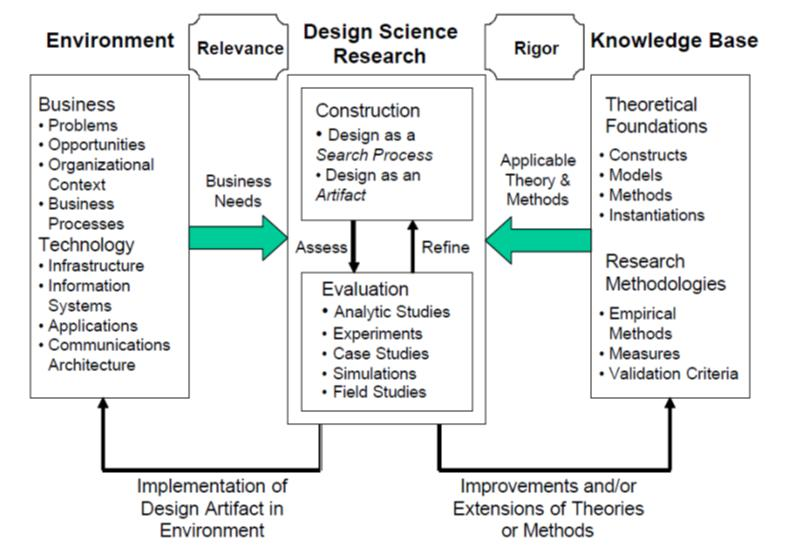
\includegraphics[width=0.7\linewidth]{./img/InformationSystemResearchFramework.jpg}
	\caption{The Information System Research Framework as designed by \cite{hevner2010design}}
	\label{fig:InformationSystemResearchFramework}
\end{figure}

In this research, a case-study is included to ensure the relevance of the new MAS framework. By comparing the model with a real-world situation, the new MAS framework can be assessed and maybe refined.

\section{Research Process}
Firstly a literature research was concluded to assess the current negotiation methods in agent manufacturing systems. Afterwards a mapping of the processes, clarification of the objectives and determination of the requirements related to the use-case was performed. It was important to define the boundaries of the context system and the evaluation method before the system was built.

Based on this framework, a mathematical model, to assess how the negotiation will concur in the multi-agent system, will be created. A simulator will be created to evaluate this method. After the creation of the model and simulator, the relevance will be assessed by it's performance.

%After the creation of the model and simulator, the relevance will be assessed by performing business analytic's. This will be done in the form of interviews on which business opportunities can be assessed.

The operational requirements should be clear then, and the theory can match the business expectations. From this, future prospects can be concluded.


%\todo{How to evaluate }
\subsection{Evaluation Method}
%\Todo{Alignen met de rest van de introductie text}
To test the final theoretical framework, a virtual simulation is to be created. The sensors/agents can be shown, including what they know and for example their gauge values. In such a simulation, the negotiation can be visualized, and proof for the (near-)optimal outcome can be shown. By having a few variable sliders on the display, a user might change some variables which would show an increase/decrease in negotiation and optimal solution time. 

Depending on the eventual data source, two evaluation methods are possible. If a ``real'' data source is available, the Key Performance Indicator (KPI) of the business will be checked. By minimizing e.g. the consumed base and acid during the production process, an improvement of the new system can be concluded.

If a ``real'' data source cannot be found, a second model is to be implemented. Using this other, probably heuristic or Linear solution, a comparison between the new method and the other method can be conducted and evaluated in aspects of speed, quality solution, and dynamicity.

\section{Research Questions}
From the research goals and process, the following research questions are concluded:
\begin{enumerate}
	\item
	How can energy and manufacturing companies use the AI concept of intelligent multi-agent systems (MAS) for the optimization of production planning incl predictive maintenance and/or process control optimization?
	\begin{enumerate}
		\item
		What is the optimal MAS framework for the optimization of production planning?
		\begin{enumerate}
			\item 
			Theoretical: Which negotiation techniques, communication protocols, knowledge models and hierarchy/coalition to optimize decision making/scheduling.
			\item
			Simulation: Compare the new framework to an old use-case using simulation results.
		\end{enumerate}
		%\item
		%What are the technical requirements for such a system?
		%\begin{enumerate}
		%	\item
		%	Internet of Things: Sensors, protocol, Industry 4.0
		%\end{enumerate}
		\item
		What is the roadmap for other industries within the industry 4.0?
		\begin{enumerate}
			\item 
			Decentralized systems vs Centralized systems
			\item
			Negotiation in manufacturing
		\end{enumerate}
	\end{enumerate}
\end{enumerate}


\chapter{Literature Study \& Theoretical framework}
\label{ch:literature}
%Overview of Manufacturing, MAS and framework.
The manufacturing industry is and will be one of the wealth generators of the world economy. A shift towards a modular production process, the 4th industrial revolution (also called Industry 4.0 transition), results in a demand for products with high quality at lower cost while being highly customized. This results in new way of controlling the production. High-performing computing, the internet, universal access and connectivity, and enterprise integration all contribute. Overall the consensus is that only the companies that fully leverage the information, its availability, the ability to exchange it seamlessly, and process it quickly, are the companies that can meet the high demand of the consumers \citep{monostori2006agent}. 

The so-called agent-based computation is a solution for many of the problems that arise from this new trend. By having autonomous agents, who can address changes adaptively and are distributed in nature, intelligent solutions are available \citep{monostori2006agent}.

In this literature review, an overview of the manufacturing processes and current agent technologies/solutions are given. Using such a decentralized agent solution is only optimal when certain process and hardware-wise requirements, are realised on the manufacturing side. We will conclude the chapter with an overview of the framework.
\cite{abedin2014agenda}


\section{Manufacturing processes}
%Overview of manufacturing. Asset management, process control incl predictive maintenance and planningxx	, Programmable logic controller, real time control
	
	A new paradigm shift in the discrete manufacturing world requires a production that is competitive but also sustainable. Most of these solutions lie in the field of Cyber-Physical systems. A Cyber-Physical entity is one that integrates its hardware with a cyber-representation as a virtual representation. By doing so, it combines two worlds: the embedded systems and the software worlds. By doing so it breaks the traditional automation pyramid, and introduces a new more decentralized way of function \citep{leitao2016smart}. This is also visualized in figure~\ref{fig:traditional-automation-pyramid1}. %By making these systems intelligent, and connecting the design principles, the current lacking of industrial can be fully leveraged.
	
\begin{figure}
\centering
\includegraphics[width=0.9\linewidth]{"img/traditional automation pyramid1"}
\caption{The breaking of the traditional automation pyramid, and future of a new more decentralized way of function. Image from \citet{monostori2016cyber}.}
\label{fig:traditional-automation-pyramid1}
\end{figure}

	The traditional automation pyramid, is very similar to the multiple layers in the manufacturing process, which has been standardised by the American National Standards Institute (ANSI) \citep{harjunkoski2009integration}. The integration of the planning and control in the manufacturing process is one that has many aspects. Below a short overview of manufacturing will be given in the ANSI structure. This goes from asset management using process control, to real time monitoring. 
	
	
	%\Todo{UItleggen wat de 4 layers zijn en zeggen dat je ze stuk voor stuk behandelt in de volgende subsections. }
	
	\begin{figure}
\centering
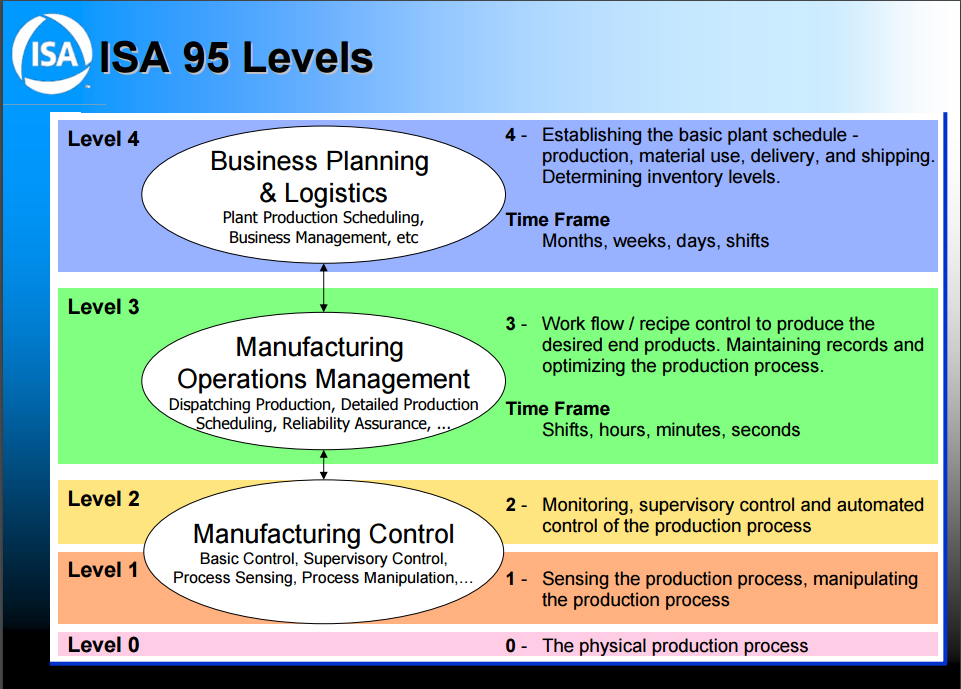
\includegraphics[width=1\linewidth]{img/ansi-isa-95}
\caption{The manufacturing levels as described and defined by ANSI for the ISA-95 levels~\citep{brandl2008ISA}. }
\label{fig:ansi-isa-95}
\end{figure}

	 
%	The term scheduling is also used in various contexts and can be closely interlinked with lots of related optimization problems, such as maintenance planning, energy and inventory optimization, cutting-stock problems in the paper mills, etc. Furthermore, the time horizon largely depends on whether the focus is on short-term, mid-term or long-term scheduling or planning \citep{pinedo2005planning}. However, in this review the term planning will be used interchangeable with scheduling.	


\subsection{Asset management}
% \Todo{Niet duidelijk hoe dit met ANSI te maken heeft, \\de hoogste laag van abstractie + gramilrieit w.b. tijd.}
	Asset Management is the broad overview of the administration of assets. This includes the design, construction, use, maintenance, repair, disposal and recycling of assets. For most corporations and enterprises, the focus lies on the operational aspects of the assets, due to the fact that asset failures result in production or service delays. Therefore, insufficient asset management on one side results in loss of the asset itself, and on the other side loss due to productions delays and loss of service \citep{trappey2013multi}.  A lot is currently being researched, for example by \citet{leitao2009agent}, on asset management, and especially the condition monitoring and prediction are in focus. This is due to the shift from reactive repair work to real-time condition monitoring, prediction, diagnostics and pre-scheduled maintenance. Also, traditional asset management approaches are poorly suited for current equipment failure solutions. %\Todo{Onderhoud + inspecction. Gebruik woord ``Asset Integrity''}
	
	Traditional manufacturing control systems are unable to be sufficiently responsive, flexible, robust and reconfigurable due to the fact that they are built upon a centralised and hierarchical control structures. These are optimal for perfect optimization, but weakly responsive to change. Another consequence of this structure is that a single failure can shut down an entire system \citep{leitao2009agent}. This requires a change to decentralized asset management, demanding for new process control methods.
	
	%If the plant's availability to produce is deteriorating, then the current production schedule is easily jeopardized and rescheduling (or even replanning) may become necessary. Plant Asset Management deals with questions around plant asset health and therefore is concerned with the ability to produce as desired. Plant Asset Management (PAM) scheduling should also include plant health information in order to take care of required maintenance options, or the other way around, the maintenance schedule should be optimally embedded into the production schedule. \cite{harjunkoski2009integration}
	
	Generally, researchers use agent-based technology to represent real world situations through the use of a computational simulation process, where agents can interact with each other to find a common goal. Typically, in these environments, agents have conflicting goals. In such circumstances, they will negotiate with each other in order to resolve conflicts \citep{rosa2009intelligent}. These methods will be described in section \ref{sec:negotiation}.
		
	
\subsection{Process control}

There are three different processing methods: discrete, batch and continuous. Each process can be defined in terms of one or more of these methods. A discrete process method is when the production results in separate pieces. These are for example created in Industrial Robotic Solutions. Each robot produces a separate product in the manufacturing process. It is one of the most used manufacturing production application.

Batch production is when specific quantities of the materials have to be combined in particular ways. These are typically food productions. An example is the beer production. In a specific batch, the ingredients are combined, and after a period we have our required product. The last process method is continuous production. This type of control is required if the variables are smooth and uninterrupted in time. The process of the creation of de-mineralized water is a continuous process. The water continuously flows through the system and finalizes in the required product with no interruptions. 

An example from \citet{engell2012optimal}, which is displayed in figure~\ref{fig:processstructure} shows the typical process control method. This is in line with the ANSI standardisation described in the introduction. %\Todo{where is ANSI described}. \Todo{Hoe correspendeert dit met ANSI?}

\begin{figure}
\centering
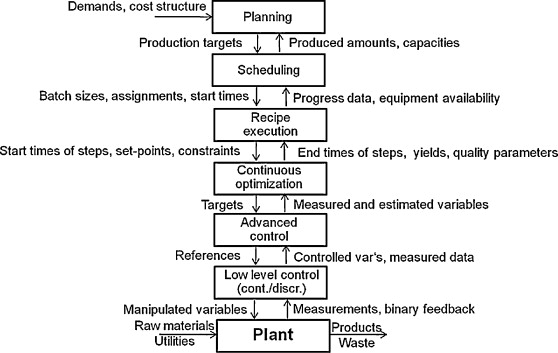
\includegraphics[width=0.7\linewidth]{img/process_structure}
\caption{Typical process structure from \citet{engell2012optimal}}
\label{fig:processstructure}
\end{figure}

\subsubsection{Planning}
Important when controlling a process is to optimize the planning. The forms of decision making used in optimization of planning play an important role in the performance of a production plant. By using different mathematical and heuristic methods, the limited resources can be correctly allocated. This optimization is essential such that the objectives and goals of a company are satisfied (or even better). By minimizing, for example, the time to complete the production, while satisfying the goals, efficiency is increased, which often results in cost reduction \citep{pinedo2005planning}. 

One of the largest difficulties when planning, is that of ensuring that the assets are always operational, or have (as short as possible) planned downtime. This is achieved with predictive maintenance.
%Planning and scheduling are forms of decision-making that are used on a regular basis in many manufacturing and service industries. Decision-making processes play an important role in procurement and production,in transportation and distribution,and in information processing and communication. The planning and scheduling functions in a company rely on mathematical techniques and heuristic methods that allocate limited resources to the activities to be done. This allocation of resources has to be done in such a way that the company optimizes its objectives and achieves its goals. Resources may be machines in a workshop,runways at an airport,crews at a construction site,or processing units in a computing environment. Activities may be operations in a workshop,take-offs and landings at an airport,stages in a construction project,or computer programs that have to be executed. Each activity may have a priority level,an earliest possible starting time and/or a due date. Objectives can take many different forms,such as minimizing the time to complete all activities,minimizing the number of activities that are completed after the committed due dates,and so on.
%
%Generic manufacturing environment and the role of its planning and scheduling function. Orders that are released in a manufacturing setting have to be translated into jobs with associated due dates. These jobs often have to be processed on the machines in a workcenter in a given order or sequence. The processing of jobs may sometimes be delayed if certain machines are busy. Preemptions may occur when high priority jobs are released which have to be processed at once. Unexpected events on the shopfloor,such as machine breakdowns or longer-than-expected processing times,also have to be taken into account,since they may have a major impact on the schedules. Developing,in such an environment,a detailed schedule of the tasks to be performed helps maintain efficiency and control of operations. 
%The shopfloor is not the only part of the organization that impacts the scheduling process. The scheduling process also interacts with the production planning process,which handles medium- to long-term planning for the entire organization. This process intends to optimize the firm’s overall product mix and long-term resource allocation based on inventory levels,demand forecasts, and resource requirements. Decisions made at this higher planning level may impact the more detailed scheduling process directly. Figure 1.1 depicts a diagram of the information flow in a manufacturing system.

\subsection{Predictive maintenance systems}
To prevent malfunctions, maintenance is necessary. However, this maintenance results in downtime, and is preferably left out, to keep operations running. This however results in the breakdown or wear-out of these systems. By using maintaining assets before they break by so called ``preventive maintenance'' this damage can be controlled. %Predictive maintenance is the next level of solutions.

The old fashioned model is corrective maintenance. Since maintenance results in the shut-down of production plans, most companies postpone the maintenance to the last moment possible. By ensuring to take as many hours as possible from the machine, the most is taken out of their investment. However, since the breakdown can happen any moment, they need a high inventory of spare parts and materials.  And usually the repair is more expensive than maintenance. %This is typically seen as putting the cart before the horse.

Preventive maintenance is the alternative to corrective maintenance. Using predetermined fixed interval planned maintenance, the asset are maintained. However, this results in the not knowing whether maintenance is planned too early, or worse, too late. How can one be assured that the maintenance timing is optimal, due to the many factors of influence on the asset (wrong usage, or external surrounding like sun, dust and rain)? Often either maintenance is done to soon, resulting in extra cost, or to late which results in the breakdown of the asset.

Condition-based maintenance is a step in the right direction. By ensuring preventive maintenance on the right moment, the machines do not breakdown and there is no overkill on maintenance. On specific intervals, the machines are measured regarding their current status and using, for example, vibration measurements or oil samples, their current condition can be assessed. Parts that have a high probability of failure can be replaced in their next maintenance or production stop. However, this is not the optimal solution: measurements are sporadically done (not continuously) and there remains the chance of failure before the maintenance stop has occurred.

Using predictive maintenance it is possible to continuously, in real-time, monitor an installation. This can be done over a distance. Currently there are assets filled with sensors which produce data. This data is shared with people, other machines and servers. This allows for predication of failures, and real-time maintenance.

Currently a lot of research is conducted on this new form of maintenance~\citep{muller2008concept}. This central analysis is done by recognizing patterns in the data which allows for prediction of possible faults. This branch of maintenance is also known as e-maintenance \citep{yu2003multi}, condition-based maintenance or intelligent maintenance~\citep{vermaak2007multi}.

%The ability of a considered system to assess its own state in order to ask for maintenance activities is the key element to enable autonomous planning and control within the general socioeconomic maintenance system. Nevertheless, the processing of maintenance tasks is limited through specific resources, accessibility, available spare parts, tasks with higher priority, etc. These actors of the maintenance system also follow internal rules and decision logics, i.e. the mitigation of costs or risks. In conclusion, entities of the socioeconomic maintenance systems require the ability to negotiate possible constellations according to their local objectives. In complex and dynamic environments this promises to gain efficiency also on the macro level because in cooperating systems the entities pursue a globally optimized behavior and want to achieve common goals. Focusing on a multi-agent-approach in order to enable this kind of negotiation and cooperating system, the different entities of the overall system have to be modeled as intelligent agents, which are able to act without the intervention of humans or other systems \cite{weiss2000multiagent}. Each agent is self-content and acts autonomously in order to enable autonomous decision-making. Within the proposed multi-agent system the planning and control is shifted from a central system with hierarchical structures to decentralized autonomously acting agents. The general problem is split into smaller problems that agents solve locally. %\cite{Towards autonomous control in maintenance and spare part logistics- challenges and opportunities for preacting maintenance concepts}

%\cite{parunak1999industrial}


%The basic goal of all maintenance policies is to prevent or forestall future random failures of the system by removing equipments from service at an appropriate time, providing unexpected zero-downtime. Currently, many developments offer various condition monitoring techniques that directly or indirectly affect the existing maintenance policies. Data acquisition systems, signal processing techniques, experts systems, e-maintenance, and web applications make the condition monitoring much more attractive and accurate. In order to integrate all the mentioned issues within the condition monitoring techniques, agent-based technology offers an interaction level that includes coordination abilities. 



%




\subsection{Real-time Monitoring}
To ensure that processes are running accordingly and continuous planning is applied, real-time monitoring is required. Essential in implementing a real-time plan or schedule is that it has to be generated in seconds on the available computer. This may be the case if rescheduling is required many times a day because of schedule deviations. This can be done in two ways. The first way is to review the overall processes and functions performed on the data in real time, or as it happens, through graphical charts and bars on a central interface/dashboard. The second method is by implementing a programmable logic controller. By automating the industrial electromechanical processes, in a predictable and repeating sequence by use of a logic ladder, a real-time controller is achievable. 

\section*{Manufacturing with agents}
When dealing with multiple processes, production and manufacturing wise, and have to keep real-time track of the assets with sensors, the most common solution lies in agent solutions~\cite{leitao2013past, monostori2016cyber}. This is often easier said than done. In the following section, an introduction in agent-solutions will be given with a focus on negotiation and manufacturing.
%
%
%Real time monitoring for continues process is a necissaty. As explaie
%Real-time data monitoring (RTDM) is a process through which an administrator can review, evaluate and modify the addition, deletion, modification and use of data on software, a database or a system. It enables data administrators to review the overall processes and functions performed on the data in real time, or as it happens, through graphical charts and bars on a central interface/dashboard.
%Techopedia explains Real-Time Data Monitoring (RTDM)
%
% fRTDM primarily helps in monitoring and managing the consumption and use of data across a complex IT system or on a standalone software/database. Typically, an RTDM software/system provides data administrators with visual insights into the data, which is fetched from various sources including Web server logs, network logs, database logs and application usage statistics. It can also provide instant notifications/alerts into specific data-driven, administrator-specified events, such as when a data value goes out of range.
%
%%\subsection{Programmable Logic Controller}
%Used for real time control is a Programmable Logic Controller. A PLC is a digital computer used for automation of typically industrial electromechanical processes, such as control of machinery used for production. PLCs solve the logic in a predictable and repeating sequence, and ladder logic allows the programmer (the person writing the logic) to see any issues with the timing of the logic sequence more easily 
\newpage
\section{Agent Solutions}
%Overview, OOP, MAS, Holonic, Negotiation, Planning/Resource allocation, Negotiation in Manufacturing -> framework. 
The new requirements in production ask for new manufacturing planning. This requires a new planning method, which is best implemented using distributed, decentralized structures \citep{parunak1999industrial}. The basis of a distributed method lies in Object-oriented programming (OOP) and Multi-Agent structures. Using these structures and negotiations planning can be optimized.

\subsection{Object-oriented programming}

Object-oriented programming (OOP) is a programming method based on the concept of ``objects'', which may contain data and code. For example an object can be a variable, a data structure, or a function, or a combination of these. The code that an object contains can be seen as the behaviour of the object, and as such it is easily interchangeable with an agent, since a method (or message) in OOP is a procedure associated with an object. An object is made up of data and behaviour, which form the interface that an object presents to the outside world \citep{shoham1993agent}. 

Agent-oriented programming is a method often used to implement a multi-agent system. In such a system anthropomorphic ideas, like beliefs, desires are used to model the objects, and thus called agents \citep{shoham1993agent}. Agents will be discussed later in this overview.% Import to note is that based on agent-based programming, see \citet{mahar2012agent} for a thorough overview, 

% 

%they are modeled after an anthropomorphic architecture, with beliefs, desires, etc. \citep{shoham1993agent} 

\subsection{Multi-Agent Systems}

Some terms used in the literature for data collection apparatus that aggregate the data are ``Smart Objects'', ``Intelligent Gateways'', ``Collaborative Network'', ``Wireless Sensor Network'' and ``Industrial Agents''. Most of these can be viewed as Multi-Agent Systems (MAS) where the sensors communicate with one another as decentralized intelligent agents for independent action performance depending on the context, circumstances or environments (sensor input) of the situation. From such MAS, Ambient Intelligence  is conceivable: real-time decentralized decision making based on real-time data acquisition, analytics and negotiations. An example structure can be seen in Figure~\ref{fig:MAS_example}.

To define MAS, an agent needs to be defined. An agent is a system that is capable of independent action on behalf of its user or owner. As  \citet{wooldridge2009introduction} formulates it, ``An \textit{agent} is a computer system that is \textit{situated} in some \textit{environment}, and that is capable of \textit{autonomous action} in this environment in order to meet its delegated objectives.'' This independent action execution is already a form of intelligence\citep{wooldridge2009introduction}. In the MAS the developer would most probably implement such intelligence by giving each agent ``Beliefs, Desires, and Intentions'' \citep{rao1995bdi}.  

Multi-agent systems (MAS) have been identified as one of the most suitable technologies to contribute to the deployment of decentralized optimization that exhibit flexibility, robustness and autonomy\citep{vinyals2010survey}. Currently there are a lot of relevant contributions regarding agent technologies to this emerging application domain. However, many challenges remain for the establishment of MAS as the key enabling technology \citep{vinyals2010survey}. A few problems, like a lack of focus on multiple owners, decision making with only available local knowledge research and lack collective sensing strategies, are still subjects that require extensive research. They see these as the possibly most active MAS research topics. Many of these problems can be solved with negotiation, which will be covered later.

\begin{figure}[h]
	\centering
	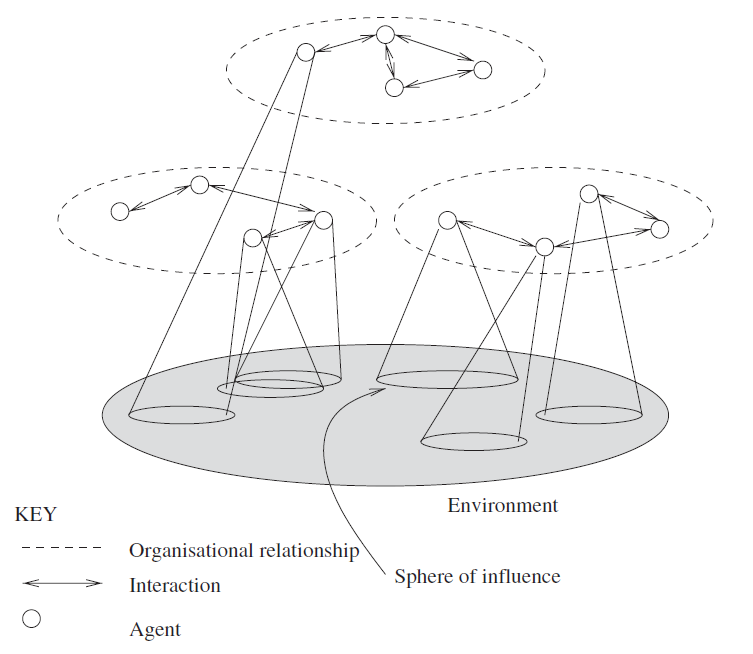
\includegraphics[width=0.7\linewidth]{./img/MAS_example}
	\caption{Typical structure of a Multi-Agent System \citep{wooldridge2009introduction}.}
	\label{fig:MAS_example}
\end{figure}

\subsection{Holonic Systems}
Multi-agent systems are composed of autonomous software entities~\footnote{The holonic structure used in our design will be explained in the chapter~\ref{ch:design}, including a visualization}. They are able to simulate a system or to solve problems. In manufacturing the requirement linked to the real-time processes resulted in a new entity and control structure: Holonic systems \citep{giret2005multi}. A holon, just like an agent, is an intelligent entity able to interact with the environment and to take decisions to solve a specific problem. Holon has the  property of playing the role of a whole and a part at the same time. The first successfully implemented holonic structure was created by \citep{van1998reference}. PROSA consisted of three types of basic holons: order holons, product holons, and resource holons. They were structured using the object-oriented concepts of aggregation and specialisation. By decoupled the system structure from the control algorithm, logistical aspects could be decoupled from technical ones. 
\begin{figure}[h]
\centering
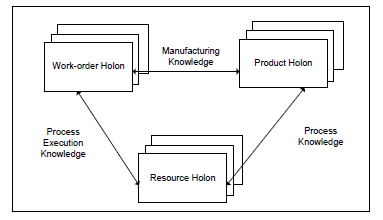
\includegraphics[width=0.7\linewidth]{img/holonic_manufacturing}
\caption{An example of an Holonic Manufacturing System (from \citet{giret2005multi}, based on \citet{van1998reference})}
\label{fig:holonicmanufacturing}
\end{figure}

\begin{figure}[h]
\centering
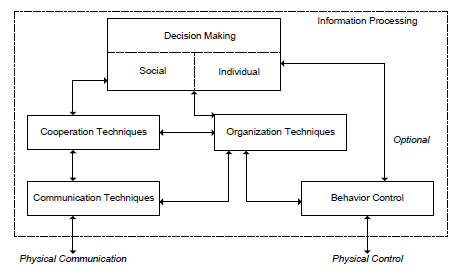
\includegraphics[width=0.7\linewidth]{img/holonic_agent_based_system}
\caption{An Holonic agent based architecture \citet{giret2005multi}}
\label{fig:holonicagentbasedsystem}
\end{figure}

The concept of holon is based on the idea that complex systems will evolve from simple systems much more rapidly if there are stable intermediate forms than if there are not; the resulting complex systems in the former case will be hierarchic. Secondly, although it is easy to identify sub-wholes or parts, ‘wholes’ and ‘ parts’ in an absolute sense do not exist anywhere \citep{van1998reference}.

\subsection{Task/resource allocation}
An example of resource allocation is when a set of agents shares a joint resource. Such a resource can be anything from indefinitely renewed continuous or discrete theoretical resource. By limiting the use of the resource to one agent at the time, negotiation is necessary to ensure that all the agents can use the resource. Usually and often crucial is the preference of the agents. Since the agents have different preferences regarding the resource, it is possible and feasible to divide the resource and create a schedule describing who has access to the resource and when \citep{fatima2014principles}. 

The same principle applies to task allocation, where the agents want to achieve a common goal. To achieve this goal quickly the agents most divide different task, which overlap, and reach an agreement on the optimal planning. 


% This paper has been concerned with how automated agents can be designed to interact effectively in both resource allocation and task distribution environments. A strategic model of negotiation has been proposed as a way of reaching mutual benefit while avoiding costly and time consuming interactions which might increase the overhead of coordination. That is, we have provided a model in which agents can avoid spending too much time negotiating an agreement and therefore are better able to stick to a timetable for satisfying their goals. In the process of developing and specifying the strategic model of negotiation, we have examined single as well as multi-agent environments, situations characterized by complete as well as incomplete information, and the differing impact of time on the payoffs of the participants. While some combinations of these factors can result in minor delays, the model nevertheless reveals an important capacity for reaching agreement in early periods of the negotiation. Throughout the paper, we have referred to two examples of application of the strategic model to problems in distributed artificial intelligence (DAI) . The resource allocation problem has been examined through the development of a scenario in which agents must share a resource in order to achieve their separate goals. The task distribution problem has been examined via a scenario in which savings can result from the sharing of tasks, and both parties benefit from cooperation. In both cases, we have met the criteria for the evaluation of a negotiation protocol which we proposed at the outset of the paper:  symmetrical distribution (no central unit or agent), efficiency (conflict avoided and no deadlocks in outcome), simplicity (process simple and efficient), stability (distinguishable equilibrium point), and satisfiability or accessibility (access to the resource or task completed). We have ended with a brief discussion of the general structure of an automated negotiator, to be based on the theoretical results of this paper. The functioning of the automated negotiator will depend upon whether it will be operating in a static or dynamic environment. The implementation of a prototype automated negotiator will provide an environment in which experimental work on the strategic model under varying initial assumptions can be undertaken, as well as one in which human negotiators can be trained. We believe that our model can be useful in other situations beside the ones we analyzed in the paper. For example, situations where there are several resources in the environment, or task distribution situations where the agents have incomplete information. We leave this for future work. \cite{kraus1995multiagent} 

%Sharing a common resource requires a coordination mechanism that will manage the usage of the resource. A coordination mechanism can be a static division of frequencies or time slots.On the other hand, it can be an on-line negotiation mechanism that dynamically resolves local conflicts over the usage of the common resource.Those are the two extreme poles of the coordination mechanism spactrum.On this spaectrum there are also coordination mechanisms that generate agreements on long term (an hour, a day, ...) global schedules. d

%As in the case of communications satellite, common resources are shared by different companies with possibly different and even conflicting goals.Therefore, to ensure efficiency, the mechanism should also be be stable and symmetric.This article formally defines these attributes and presents symmetric, stable and simple on-line coordination mechanisms that resolve local conflicts without delay and result in an efficient joint usage of the resource.

%The link between intelligent agent and game theory is established. The intelligent agents apply game theory to develop strategies that are essential in implementations of the users' tasks. Various stages of analyzing, reasoning, understanding, evaluating, predicting and executing an action must be performed by applying an optimal strategy for optimum results.

%Under some conditions, there will be convergence towards a state of equilibrium which is Pareto optimal, i.e., there exists no solution that makes some agent better off yet does not make some other worse off
%\subsubsection{Automated Negotiation}
% fipa FIPA Agent Communication specifications deal with Agent Communication Language (ACL) messages, message exchange interaction protocols, speech act theory-based  communicative acts and content language representations.
\label{sec:resourceallocation}
%Such an agents has b firstly beliefs that agent have information about their environment with may be incomplete or in correct; secondly goals, that agent will try to achieve; thirdly actions that agent perform and the effects of those actions; finally ongoing interaction that how agent interact with each other's and their environment over time. For this reason the state of an agent is called its mental state. The mental state of agents is described formally in an extension of standard epistemic logics: besides temporal the knowledge and belief operators
\subsection{Scheduling and planning}
Since most Process Planning and Scheduling (PPS) problems are NP-hard problems, many MAS have also been deployed to ``solve'' such problems in reasonable time. NP-hard (nondeterministic polynomial) problems are those problems which are at least as hard as the hardest problems in NP. This means that it is possible to reduce the problems in NP to the original problem in polynomial time. Using the decentralized global optimization approach a (sub-optimal) solution can be found. This solution would be found faster than when using an (mixed) integer program~\citep{feng2014multi}. It does however depend on the practical application of the system to see whether it is an NP-hard problem. Furthermore, this does not guarantee an optimal solution, rather that a reasonable solution will be found in reasonable time.

Real-world scheduling problems are usually complex and involve many approaches to find sub-optimal rather than optimal solutions using reasonable computing resources. The Bus Maintenance Scheduling Problem \citep{zhou2004bus}, which is distributed and dynamic in nature, has received less attention compared to scheduling problems in manufacturing. In the Bus Maintenance Scheduling Problem \citep{zhou2004bus} a MAS is proposed to heuristically solve the bus maintenance scheduling problem investigated here. It is shown that with equal optimality and less computing time without constraint violation it is comparable to the work of a mathematical programming approach.

It is also shown in \citet{bruccoleri2005production} that the agent based approach out performs the centralized mixed integer programming solution for the planning of a production.

Another example is the agile development with a MAS \citep{rabelo1999multi}. Agile development is based on the idea that requirements and solutions evolve through collaboration between self-organizing, cross-functional teams. Agile development promotes adaptive planning. By using a MAS for Agile planning, it has been shown that \textit{``the scheduling agility can be extremely improved once it is based on the following key points:
	\begin{itemize}%[i]
		\item
		distributed and autonomous systems instead of the centralized and non-autonomous solutions;
		\item 
		negotiation-based decision making instead of the totally pre-planned processes;
		\item
		application of different problem-solvers in the same environment instead of only one fixed problem solver;
		\item
		concurrent execution instead of the sequential processing''~\citep{rabelo1999multi}.
	\end{itemize}
}

Each agent is part of a heterogeneous system and processes its own information and has its own particular capabilities that it exchanges to the system. In this matter it contributes to finding a solution to the global problem which works very well in complex environments. Optimization of scheduling in such complex environments is highly constrained, with which advanced analytics also has great difficulty. Using the dynamic, flexible and intelligent relaxation of the constraints within the distributed knowledge of the agents, autonomous intelligent decision making as a Multi-Agent System is achieved \citep{rabelo1999multi}. 

% A major difficulty with classical scheduling systems is handling of conflicts. Several problems can arise during the schedule generation, after its generation, and during its execution, such as the temporal, capacity, or technologic conflicts. These problems may come from the planning, scheduling or execution supervision activities. There are several methods that can be applied for the conflict resolution in a multi-agent system. HOLOS uses the Contract-Net Protocol coordination mechanism to support the task assignments to agents, and the Negotiation [7], [17] method to overcome conflicts taking place during one of the three mentioned scheduling phases \cite{rabelo1999multi}

%\section{Agent Technologies}
\
\section{Negotiation}
\label{sec:negotiation}
Often discussed above is the negotiation of the agents in a multi-agent system. This branch of research, also called automated negotiation, is studied by Artificial Intelligence and Economics \citep{jennings2001automated}. Concepts from fields such as decision theory and game theory can provide standards to be used in the design of appropriate negotiation and interaction environments \citep{jennings2001automated}. It is used to reach an agreement that meets the constraints of two or more parties in the presence conflicting interests. And thus is a basic means of getting what you want from others \citep{fisher1987getting}. It is back and forth communications designed to reach an agreement when you and the other side have some interests that are shared, and others that are opposed. Agents reason rationally and strategically. An agent's objective is to maximize the expected value of its own payoff. 

The four components of a negotiation model are~\citep{fatima2004agenda}:
\begin{enumerate}
	\item The negotiation protocol.
	\item The negotiation strategies.
	\item The information state of agents.
	\item The negotiation equilibrium.
\end{enumerate}

Since negotiating situations occur when there is a conflict of interest, the first step will be to detect such a conflict. Agents will use communication channels and try to eliminate the conflicts. Conflicts may be about limited available resources, or may be a conflict between the beliefs of some agents. In the first case, optimization is the result, whereas, in the second case, one of the agents will have to change its beliefs \citep{shen2003multi}. Often it is seen as maximizing the quality of the result. Two solutions are possible, one, the agents can try to achieve Pareto optimality, meaning that the outcome maximizes the product of the agents' utilities, or they try to reach a Nash equilibrium, meaning an stable state in the system, both which will be discussed in the evaluation method.

Negotiation is done by exchanging messages among agents. Since the process involves several messages, a discussion will take place in which each agent's belief and goals will be an important factor. These depend on the global situation. Clearly, to be able to negotiate, agents must be able to reason. Thus, negotiation is restricted to cognitive agents. Automated negotiation is essentially a distributed search in the space of potential agreements between the different negotiators represented by autonomous agents, which involves the exchange of relevant information and aims to find an agreement that is acceptable to all participants.

Negotiation domains, can be divided into task orientated domains (TODs), state orientated domains (SODs) and worth orientated domains (WODs). TODs are the simplest and an agent's activity is defined in terms of the set of tasks it has to achieve. It is assumed that all resources are available, the benefit of negotiation is the redistribution of tasks amongst a group of agents which results in a more efficient task order. A typical example is mail delivery where an agent may carry another agent's mail at little extra cost. It is sertain that the states come closer to a Pareto optimal solution as all agents can proceed with their original task list and be no worse off. SODs deal with problem where agents wish to change their environment from an initial state to some goal state. The classic AI Blocks World problem is a good example. There is the possibility of conflict and dead end, since the agents may have different goals, and it is not feasible to try and satisfy these goals all for all agents. In this situation, agents must be able to make concessions. WODs are domains where agents attach a worth to each potential state. This allows much more flexible goals to be set and allows concessions to be made on these goals. An example would be agents in an marketplace where the goal for a seller may be to obtain the highest price for x within time y. There is again the possibility of conflict and deadlock, but now within a more complicated bargaining environment \citep{anumba2003negotiation, fatima2014negotiation} .

\subsection{Negotiation Protocol}
Negotiation Protocol is the set of rules that govern the interaction and defines who are the actors of the negotiation, the states that characterize a trade (for example, when a negotiation has begins or ends), the events that determine the change of actors’ status, and messages that can be sent by the actors in a particular state. This however is no easy task, since there is no one size fits all solution. Some attempts have been made, by \citet{marsa2014problems} for example, and a collection of design rules which allow, given a particular negotiation problem, to choose the most appropriate protocol to address it. However, these problems are only derivable when (1) the negotiation domain, including the issues and possible issue values, (2) a scenario utility histogram, which defines the distribution of contracts in utility space, and (3) several structural parameters that specify the topography (e.g. ruggedness) of each agent's utility function are known. In the design of the system, this will be discussed.

The most important protocol is that of the alternating-offers protocol \citep{rubinstein1982perfect} \todo[Rubenstein uitleggen]{Rubenstein uitleggen}. It is based on a divisible pie, discrete or continuous, and is the most widely studied among game-theorist as well as MAS researchers \citep{fatima2014principles}. Other examples is the contract net protocol and the bargaining protocol. 

A typical negotiation protocol is very similar to that of our negotiations in our everyday life and work. Thus, a negotiation typically proceeds over a series of rounds, with one or more proposals being made at each round. It also includes the rules that impose the constraints on the rules and the rule that shows when a deal has been struck \citep{fatima2014principles}. Different negotiation mechanisms need to be developed to suit the different application environments of MAS. Unlike the negotiations between human beings which involve more complex human interactions than simple technical issues, the negotiation mechanisms between agents are rule-based or case-based. Yet, the human negotiation approaches and theories, which mainly include game theory and behaviour theory, provide sound bases for the negotiations between agents. 

Another common protocol is the monotonic concession protocol. It is a proposal which has also been adapted for multi-lateral negotiation in \citep{endriss2006monotonic}.



\subsection{Negotiation Strategies}
The strategy can be defined formally as an apparatus which allows the agent to determine the content of the action that it will perform consistently with the protocol. In general, for a given set of negotiation protocol there are many strategies compatible with it, each of which can determine a different action. This means that a strategy can work well with a given protocol, but does not work with others. So, the choice of strategy depends on the protocol in use and by the trading scenario \citep{di2015multi}.

Often these strategies are private, meaning that not all the agents can see what the strategy of an agent is \citep{fatima2004agenda}. Example of a strategy is the Zeuthen strategy which results in the outcomes being equivalent to the Nash bargaining solution. 

\subsubsection{Concession Strategy}
\label{sec:concessionstrat}
\todo[Hier concession uitleggen]{Concession uitleggen!!}

\citet{endriss2006monotonic} devines 7 different concession strategies, to increase utility. 

\citet{wu2009efficient} describes 4, for resources allocaiton. 


\subsection{Negotiation States}
An agent’s information state describes the information it has about the negotiation game. There are two possibilities, states with complete information and those of incomplete information. The first category is basic and most common. In these games the players are assumed to know all the information about the rules of the game and the players their preferences. However, in the incomplete category, information may be lacking about a variety of factors in the problem \citep{fatima2004agenda}. %\Todo{What is the implication of this?}

%Since there is no one negotiation protocol that clearly outperforms all others in all scenarios, we need to be able to decide which protocol is most suited for each particular problem. The goal of our work is to meet this challenge by defining a “negotiation handbook”, that is, a collection of design rules which allow us, given a particular negotiation problem, to choose the most appropriate protocol to address it. \cite{marsa2014problems}
%Clearly, to be able to negotiate, agents must be able to reason. Thus, negotiation is restricted to cognitive agents
% In multi-agent systems automated negotiation is used to model the process of decision making to reach an agreement that meets the constraints of two or more parties in the presence conflicting interests. The conflict of interest refers to the fact that agents have conflicting interests, as in the case that occurs between a seller and buyer. As described in [32], automated negotiation is essentially a distributed search in the space of potential agreements between the different negotiators represented by autonomous agents, which involves the exchange of relevant information and aims to find an agreement that is acceptable to all participants. In the following the main features which characterize the automated negotiation are described: 

%Negotiation Protocol is the set of rules that govern the interaction and defines who are the actors of the negotiation, the states that characterize a trade (for example, when a negotiation has begins or ends), the events that determine the change of actors’ status, and messages that can be sent by the actors in a particular state. 
%Negotiation Object is identified by the set of parameter values which must be reached for an agreement, known as Agenda [23]. To dynamically change the agenda by adding or removing parameters may be allowed by the protocol.
%Bidding Strategies (model of decision making agent) can be defined formally as an apparatus which allows the agent to determine the content of the action that it will perform consistently with the protocol. In general, for a given set of negotiation protocol there are many strategies compatible with it, each of which can determine a different action. This means that a strategy can work well with a given protocol, but does not work with others. So, the choice of strategy depends on the protocol in use and by the trading scenario.

%Automated negotiation occurs when software agents negotiate on behalf of their human counterparts. It has been studied in artificial intelligence and electronic commerce for many years [4], [10]. Jennings et al. [5] argue that negotiation is the most fundamental mechanism to manage runtime dependencies among agents, and thus underpins cooperation and coordination. Lomuscio et al. [10] argue that automated negotiation underpins the next generation of electronic commerce systems, and develop a classification scheme for negotiation in electronic commerce. It offers a systematic basis on which different negotiation mechanisms can be compared and contrasted.

%Automated negotiation has been proposed as an ideal approach to procure cloud resources and services. Sim [16] proposes a market-driven, agent-based negotiation mechanism to procure resources and services in the cloud marketplace. In particular, the mechanism supports parallel negotiation activities, namely, multiple negotiations at the same time. It is reported that with it, agents can achieve more utility and a high success rate. Stantchev and Schröpfer [17] propose an approach for SLA mapping between business processes and IT infrastructures. It aims to formalize, negotiate, and enforce QoS requirements for cloud services. However, no negotiation approaches are specified. Yaqub et al. [29] present a generic negotiation platform for SLA@SOI (Service-Oriented Infrastructure). However, it focuses on negotiation protocols and not the negotiation strategies that we deal with in this paper. \cite{zheng2014cloud}

%anumba DOMAIN Rosenschein and Zlotkin [35] divide negotiation domains into task orientated domains (TODs), state orientated domains (SODs) and worth orientated domains (WODs), with each domain being a generalisation of the previous. TODs are the simplest and an agent's activity is defined in terms of the set of tasks it has to achieve. It is assumed that all resources are available, the benefit of negotiation being the redistribution of tasks amongst a group of agents. A typical example is mail delivery where an agent may carry another agent's mail at little extra cost. There is no possibility of deadlock as all agents can proceed with their original task list and be no worse off. SODs deal with problem where agents wish to change their environment from an initial state to some goal state. The classic AI Blocks World problem is a good example. There is the possibility of conflict and deadlock, as agents may have different goals, and satisfy all may be impossible or require more effort from each agent than if they were alone in the world. In this situation, agents must be able to make concessions. WODs are domains where agents attach a worth to each potential state. This allows much more flexible goals to be set and allows concessions to be made on these goals. An example would be agents in an electronic marketplace where the goal for a seller may be to obtain the highest price for x within time y. There is again the possibility of conflict and deadlock, but now within a more complicated bargaining environment.\cite{anumba2003negotiation} 

%anumba MECHANISM Different negotiation mechanisms need to be developed to suit the different application environments of MAS. Unlike the negotiations between human beings which involve more complex human interactions than simple technical issues, the negotiation mechanisms between agents are rule-based or case-based. Yet, the human negotiation approaches and theories, which mainly include game theory and behaviour theory, provide sound bases for the negotiations between agents. 

%anumba Besides choosing the key negotiation approaches, there are many other factors that need to be addressed based on the application scenario. Kraus [20] explains that there are five issues which need to be further determined if game theory is selected as the basic negotiation mechanism. They are: choosing a strategic bargaining model which is applicable to the problem; matching the scenarios with the game-theoretic definitions of the chosen model; identifying equilibrium strategies; developing low complexity techniques for searching for appropriate strategies; and providing utility functions.


%Negotiation is a dialogue between two or more people or parties intended to reach a beneficial outcome. This beneficial outcome can be for all of the parties involved, or just for one or some of them, in situations in which a good outcome for one/some, excludes the possibility of a desired result for the other/others. And is aimed to resolve points of difference, to gain advantage for an individual or collective, or to craft outcomes to satisfy various interests. It is often conducted by putting forward a position and making small concessions to achieve an agreement. The degree to which the negotiating parties trust each other to implement the negotiated solution is a major factor in determining whether negotiations are successful. Negotiation is not a zero-sum game; if there is no compromise, the negotiations have failed. When negotiations are at an impasse it is essential that both the parties acknowledge the difficulties, and agree to work towards a solution at a later date. Negotiation occurs in business, non-profit organizations, government branches, legal proceedings, among nations, and in personal situations such as marriage, divorce, parenting, and everyday life. The study of the subject is called negotiation theory. Professional negotiators are often specialized, such as union negotiators, leverage buyout negotiators, peace negotiators, hostage negotiators, or may work under other titles, such as diplomats, legislators or brokers.

%The study of automated negotiation play an increasingly important role in society.Since informations and tasks are shared in distributed enviornment and agents have limited functionality, it will be necessary to consider ways in which these agents can be made to interact for resourses and/or information effectively.


% Since there is no one negotiation protocol that clearly outperforms all others in all scenarios, we need to be able to decide which protocol is most suited for each particular problem. The goal of our work is to meet this challenge by defining a “negotiation handbook”, that is, a collection of design rules which allow us, given a particular negotiation problem, to choose the most appropriate protocol to address it. \cite{marsa2014problems}

\subsection{Evaluating /equilibrium solutions}
When evaluating the dilemmas of a negotiation between agents essential is the Pareto-Frontier. Visualized in figure \ref{fig:paritooptimal}, it is used to determine whether an outcome of a negotiation is efficient. This means that no improvement can be achieved for all agents. 
\begin{figure}
	\centering
	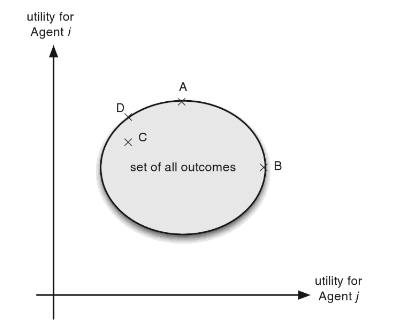
\includegraphics[width=0.7\linewidth]{img/parito_optimal}
	\caption{An example of Pareto optimal. Locations A and B are optimal, since no improvement, without loss for the agents, is possible. C and D are not optimal. From \citet{fatima2014principles}.}
	\label{fig:paritooptimal}
\end{figure}

The Nash equilibrium is the best reply to the other players strategies. This means that if both players play their Nash strategy, neither will have the incentive to change their method. Different equilibria are possible and shown in figure \ref{fig:majorcategoriesofgametheory}. 

\begin{figure}
	\centering
	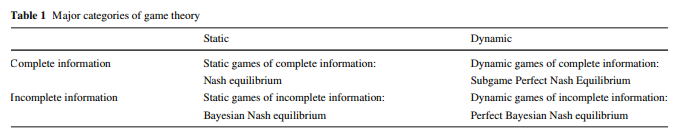
\includegraphics[width=1\linewidth]{img/major_categories_of_game_theory}
	\caption{The four types of games in game theory from \citet{trappey2013multi}.}
	\label{fig:majorcategoriesofgametheory}
\end{figure}


\subsection{Principled Negotiation}
An example of a common method for negotiation is principled negotiation. This method developed by \citet{fisher1987getting} was founded on the idea that negotiators could reach better agreements by finding favourable agreements. By focussing on interests not positions and using objective criteria, an agreement is more likely to be reached. This method has successfully been deployed in a Multi-Agent System for air traffic management~\citep{wangermann1998principled}. Emphasised is the fact that it is important to agree on objective criteria for assessing options~\citep{fisher1987getting}. If an agreement can be reached using this criteria, it is more likely that it is rational. Furthermore it is useful for systems in which no agent has global knowledge of the system. 

The purpose of this type of negotiation is to help to reach agreement without jeopardizing the business relations. It was created by \citet{fisher1987getting} and they refer to this kind of agreement as a wise agreement. Wise agreement is agreement that meets the interests of both parties to the extent possible, is long lasting, and also considers the interests of the larger society. The basis of this negotiation principle is to separate the relationship issues from the problem issues, to focus on interests not on positions, while trying to be creative in developing solutions.

% \cite{wangermann1998principled} Principled NegotiationI was developed as a method that negotiators could use to reach better agreements than could be obtained using traditional confrontational tactics. The underlying idea is that in most situations there are options that will benefit all the parties in negotiation. A favorable agreement is more likely to be reached if a negotiator proposes options for mutual gain and if all the parties assess the options using objective criteria (Fig. 3). Traffic management agents would be able to a.pprove many of the proposals, as the proposing agent would try to ensure that the options provided mutual gain. 






%\subsubsection{Example}


%\todo{Breder trekken qua literatuur}%In a cooperative negotiation, agents are allowed to communicate and to receive side payments. Furthermore, in cooperative games, agents can make binding commitments. These cooperative games result in coalitions which can be used to solve some of the problems that occur from the prisoners dilemma. 

%Within negotiation there are several more methods~\cite{wooldridge2009introduction}:
%\begin{itemize}
%	\item Patient players;
%	\item Impatient players;
%	\item Negotiation decision functions.
%\end{itemize} All these methods can be used to negotiate/bargain for resource allocation. More examples are available which will also be analysed in the in-depth literature review.

%Several other communication techniques might be useful for decision making~\cite{wooldridge2009introduction}:
%\begin{itemize}
%	\item
%	Arguing;
%	\item
%	Public vs private announcement;
%	\item
%	Contract net protocol \cite{smith1980communication}.  
%\end{itemize}

%Contract net protocol is a form of cooperative distributed problem solving that will be discussed in the scheduling section (Section~\ref{sec:AIscheduling}).
%\subsubsection{Framework}
%An overview of these different methods is in Fatima et al.~\cite{fatima2014principles}. Unfortunately this book is still lacking. 
\subsection{Hierarchy and Voting}
Voting is a form of group decision making. The agents participating in the voting will take into account their own preferences as well as those of others when making decision about how to vote. This will often have a strategic flavour. By aiming to rank or order the candidates, a group decision can be made.

Another option are auctions, a popular mechanism to reach an agreement within the allocation of resources to agents. Examples include English auctions, Dutch auctions, Vickrey auctions and First-price sealed-bid auctions \citep{wooldridge2009introduction}. Interaction between a large number of low-level agents results in a complex system behaviour which is difficult to understand, to control and to predict. Structuring the agents in a hierarchy is the appropriate solution to tackle this complexity \citep{van1998reference}.

\subsection{Mapping of negotiation protocols}
An attempt at the visualization of the different negotiation techniques is strived at. Three variables are decided on. Single- vs Multi-Issue negotiation; bi- vs multi-lateral negotiation, and; perfect vs imperfect negotiation.  
\begin{figure}[h]
	\centering
	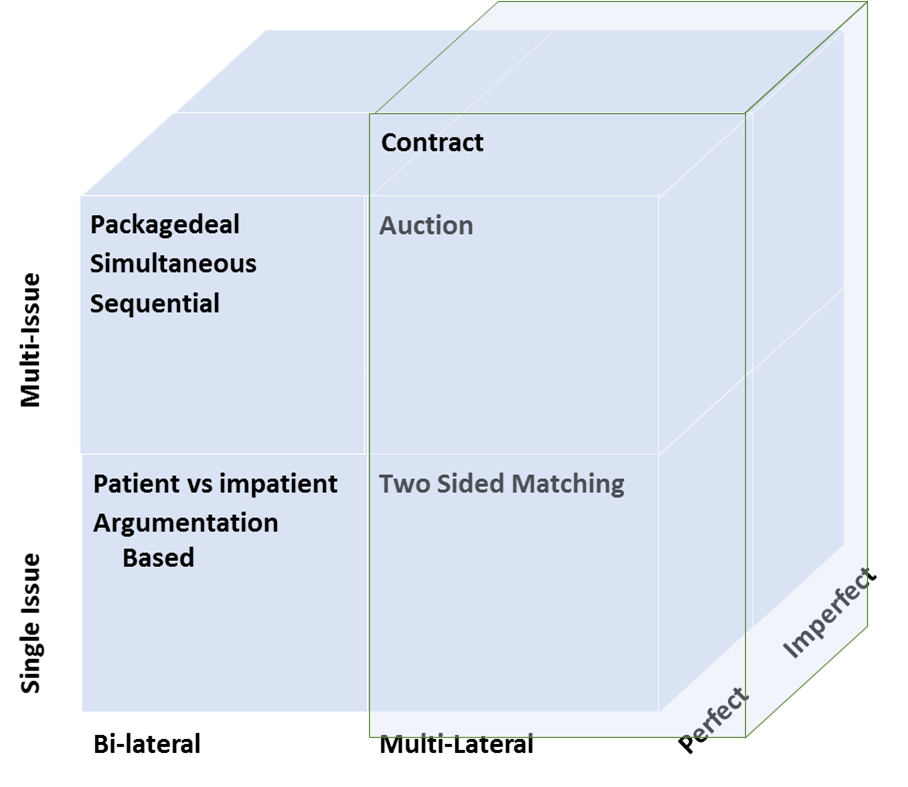
\includegraphics[width=0.7\linewidth]{img/mapping_nego}
	\caption{Current Negotiation overview}
	\label{fig:mapping_nego}
\end{figure}


\begin{figure}[h]
	\centering
	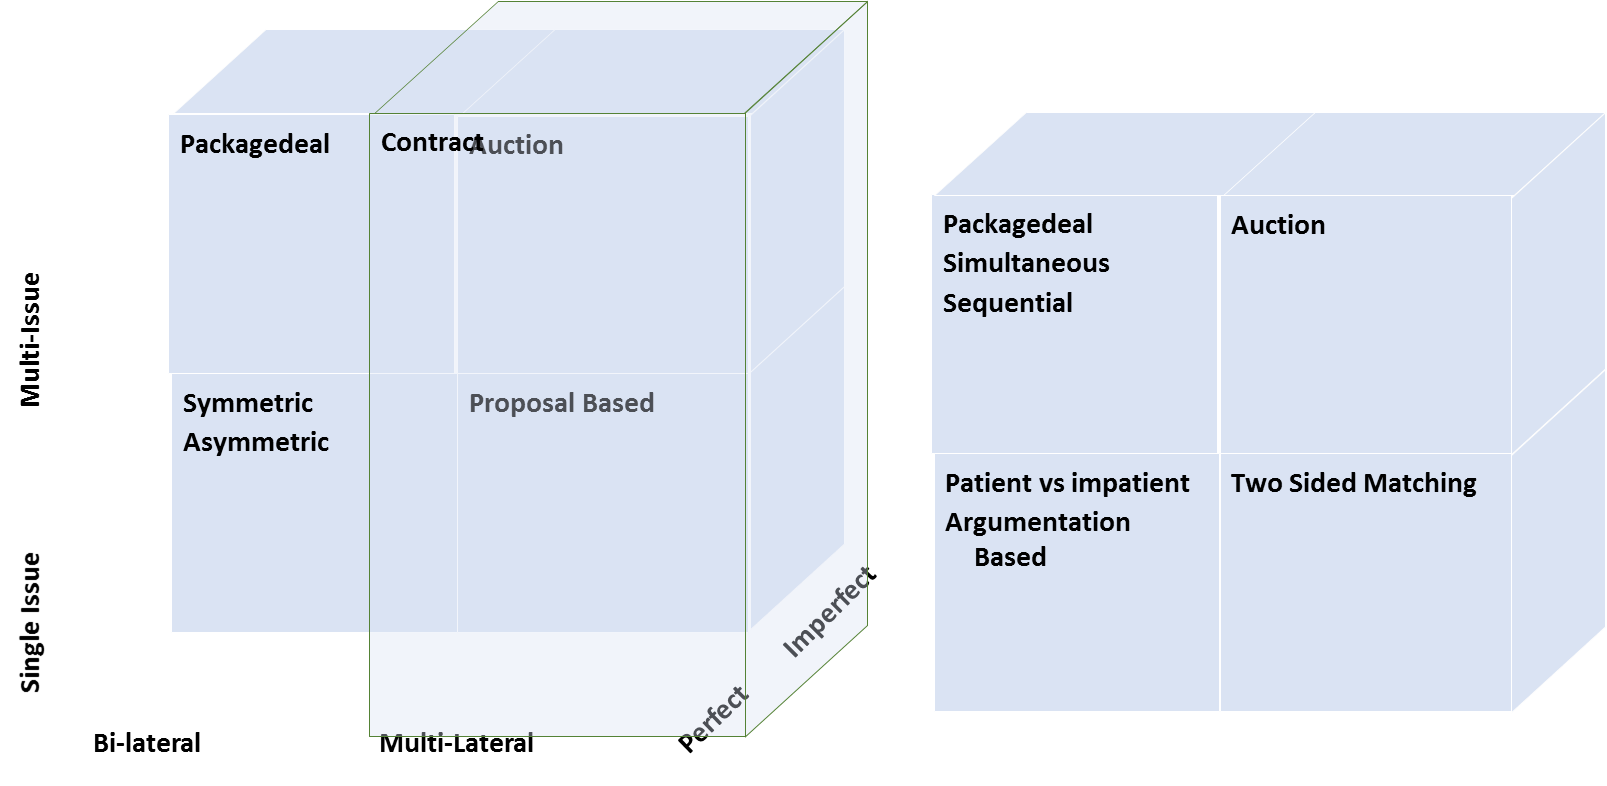
\includegraphics[width=0.9\linewidth]{img/mapping_nego2}
	\caption{Current Negotiation overview}
	\label{fig:mapping_nego2}
\end{figure}

\subsubsection{Single-Issue}

Negotiation among self-interested agents has been studied from the perspective of game theory. This is most obvious when the agents negotiate on single issues. An example might be the price of a product. When dealing with a single issue there is only one goal for both agents and there must be a conflict. If there was no conflict, no negotiation would be necessary. Typical single issue methods are patient vs impatient players, two sided matching. Argumentation based methods, which are based on the beliefs of an agents are also included in the mapping.

Essential is that all these methods are a form of the alternating offers protocol. Depending on the sort of players, the method result in completely different behaviours. These negotiation can either be complete or incomplete meaning that all information is known, or not all. 

When the game is complete, all the agents know all the information about their states and the strategies of other agents. When not all is known, the game is incomplete. The idea of negotiation is that we have an incomplete game, since if the strategies are known, most negotiation would not be necessary.

When looking at perfect vs imperfect information, it means that either the information states of the agents is perfect, meaning that the agent is perfectly informed of all the events that have previously occurred and actions (like chess), or that not all actions are known. Depending on the implementation of the system, with for example public and private announcements, the difference is made. 

When looking at single issue negotiation, depending on whether the negotiation happens between 2 (bilateral) or more (multi-lateral) agents, there are a few protocols possible. Bilateral negotiation can be either patient or impatient \citep{fatima2014negotiation} meaning that an agent has a initiative to limit the time of negotiation. Most negotiation in the manufacturing are time restrained, thus impatient agents must be implemented \citep{kraus1995multiagent}. In symmetric vs asymmetric the players are uncertain about the other players utility functions (as is the case in imperfect negotiation), but essential is that one agent might know more than the other in the asymmetric protocol.

\subsubsection{Multi-Issue}
 When negotiating multi-issues, agents attempt to combine 2 or more issue in their discussing. An example is the typical seller, buyer relationship between two agents, as for example shown in \citet{schramm2013bilateral}. Here a supply chain construction company is used to asses an method to support bilateral negotiation. Aspects like price, quality and lead-time are considered as issues, on which can be negotiated. Most used multi-issue method, for single-lateral negotiation is the package deal method. In this method, complete packages with all the issues are provided. These can be discussed either sequentially or simultaneously. 

 Agents can employ either an issue-by-issue (one-at-a-time) approach, or a packaged approach in the negotiation agenda \citep{fatima2004agenda}. In \citet{abedin2014agenda} a packaged approach for this is lack of knowledge about the opposing agents. As one issue is settled, the agent subsequently negotiates the other pending issues. This allows the agent to be cautious and opportunistic at the same time. For a multi-issue negotiation under incomplete information settings, the ideal solution is one that is Pareto optimal. A solution is said to be Pareto optimal if no agent can be better off without sacrificing the other’s utility as will be discussed in the evaluation.
 
 \begin{figure}
\centering
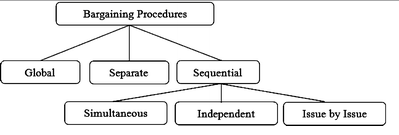
\includegraphics[width=0.7\linewidth]{img/multi-lateral}
\caption{An overview of the different negotiation method for multi issues bargaining. From \citep{abedin2014agenda}.}
\label{fig:multi-lateral}
\end{figure}
When choosing the preferred method of negotiation, important to realize is the solution required. As explained above, the issue-by-issue approach has a higher chance of optaining the Pareto optimal solution. Furthermore, the majority of the existing work on multi-issue negotiations focuses on the negotiation strategy, assuming the agenda and the procedure to be predetermined \citep{fatima2004agenda, lai2004literature}. Interesting to determine would be the influence of the domain and protocol since, depending on the scenario under which the negotiation is taking place a supervised agenda procedure can have a positive impact on the outcome of the negotiation when compared to a procedure without use of an agenda. \citep{abedin2014agenda}.


% 
 %The agenda based approach specifies how the issues will be settled. Agents can employ either an issue-by-issue (one-at-a-time) approach, or a packaged approach in the negotiation agenda (Fatima et al. 2004). We have adopted the former; negotiation one issue at a time. The main reason for this is lack of knowledge about the opposing agents. As one issue is settled, the agent subsequently negotiates the other pending issues. This allows the agent to be cautious and opportunistic at the same time. For a multi-issue negotiation under incomplete information settings, the ideal solution is one that is Pareto optimal. A solution is said to be Pareto optimal if no agent can be better off without sacrificing the other’s utility (Wilkes 2008). So the proposed negotiation approach should be able to generate Pareto optimal solutions for multi-issue negotiations. The majority of the existing work on multi-issue negotiations focuses on the negotiation strategy, assuming the agenda and the procedure to be predetermined (Fatima et al. 2004; Lai et al. 2004). Depending on the scenario under which the negotiation is taking place a supervised agenda procedure can have a positive impact on the outcome of the negotiation when compared to a procedure without use of an agenda. \cite{abedin2014agenda}

% Issue by issue negotiation gives a high probability to find a negotiation zone in an incomplete information setting rather than package and simultaneous approach. In package and simultaneous negotiation approach, the agents have limited confident and information about each other, the issues, offers and preferences. With issue by issue negotiation, there can be different agendas. Generating the optimal agenda for both agents helps to maximize their utilities. A simple but useful interdependency mechanism is derived to handle the correlation between the issues. \cite{abedin2014agenda} 

% First, in a multi-attribute negotiation the preference of an agent over multiple issues can be complex. A traditional way to deal with this is to characterize the preference with a utility function (a mathematical formula) and agents make decisions based on this utility function. However, it is not trivial for a human to construct such a utility function over multiple issues, especially when preference over one issue is impacted by the values of other issues; thus, preference elicitation may take a long time or sometimes be intractable. Second, in a multi-attribute negotiation the solution space is n-dimensional (n>1) rather than a single dimensional line as in a single-attribute negotiation. This makes the negotiation strategy in multi-attribute negotiations complex: because the space is ndimensional, every time an agent plans to concede, she needs to first decide the direction of concession. Apparently there are many choices on the concession direction she can take: to concede on issue 1, …, n or different combinations of the issues. Specifically, the decision on the concession direction may also depend on the opponent’s preference because conceding on the issue more important to the opponent can make the offer more acceptable. Finally, to decide how much to concede is now more complicated because the direction can impact the amount as well. So the burden of computation and reasoning for the negotiation strategy is higher in a multi-attribute negotiation than in a single-attribute negotiation. Third, as mentioned above, in multi-attribute negotiations there exist “Win-Win” situations. For rational agents, they should not “leave extra money on the table”. In other words, the ideal result for the system is to realize a Pareto-optimal (or Pareto-efficient) solution. A Pareto-optimal solution is one which can not be improved further without sacrificing someone’s utility, i.e. if there is another solution from which one of the agents can get more than from this Pareto-optimal solution, then the other agent must get less by that other solution. We say a multi-attribute negotiation model is efficient when agents will reach a Pareto-optimal agreement in the negotiation, if there exists a zone of agreement. \cite{lai2004literature}

\subsubsection{Multi-lateral}
The most common used method for multilateral negotiations are contract based methods, most popular being the contract net protocol. Contract net protocol by \citet{smith1980communication} is based on the principle that agents, each with a distinct expertise, can solve sub problems that are required to solve the global problem. This form of cooperative distributed problem solving is based on the assumption that agents in a system implicitly share a common goal, and thus that there is no potential for conflict between them.

Each agent (manager) having some work to subcontract broadcasts an offer and waits for other agents (contractors) to send bids. After some delay, the best offers are retained and contracts are allocated to one or more contractors who process their subtasks. The contract-net protocol provides for coordination in task allocation. 

The protocol is best suited to problems in which it is appropriate to define a hierarchy of tasks. Such problems lend themselves to decomposition into a set of relatively independent subtasks with little need for global information or synchronization. Individual subtasks can be assigned to separate processor agents. The main contribution of the contract net protocol is the mechanism it offers for structuring high-level interactions between nodes for cooperative task execution. Negotiation can be used at different levels of complexity. At one extreme, it is a means of achieving task distribution with distributed control and shared responsibility for tasks to maintain reliability. At the other extreme, the twoway transfer of information and mutual selection attributes of negotiation  make possible a finer degree of control in making resource allocation and focus decisions than is possible with traditional mechanisms \citep{smith1980communication}.

Since the contract net protocol has the uncertainty of matches being stable, the protocol of two-sided matching has been developed. Furthermore it is not certain that the matches are Pareto optimal. Using the two sided matching method, this uncertainty can be avoided, however, this protocol is harder to implement due to the fact that a clear allocation division is required. \citep{fatima2014principles}.
 
If the game is imperfect two sided matching does not work, and a proposal based protocol is the right fit \citep{rahwan2003argumentation}.


%\subsubsection{Reasoning about ones interest}
%Interest-based negotiation (IBN) is a form of argumentation-based negotiation in which agents exchange (1) information about their underlying goals; and (2) alternative ways to achieve these goals \cite{rahwan2009formal}. 


\subsubsection{Heuristic methods in negotiation}
Most of the negotiation in manufacturing can be seen as multi-lateral multi-issue negotiation. Three important distinctions are to be made, based on \citet{lai2004literature}. 
\begin{enumerate}
	\item
	issue by issue negotiation;
	\item
	multi-issue cooperative negotiation;
	\item
	multi-issue negotiation with heuristic methods.
	\end{enumerate}
	
	The first aspect looks at the agreement which is built through a strategy, and examines this individually and interactively, and the parties are considered as non-cooperative and they are built for environments with incomplete and asymmetric information, where an agenda containing the order in which issues are treated is needed. For the second aspect a multi-issue concession strategy is used whose parties are considered cooperative and they have complete and symmetrical information about their environments. These two aspects have been discussed in the sections above. In the last type, an agreement is reached through a hybrid negotiation strategy, which uses the first two types of theoretical framework with the focus in automated models based on autonomous agents for multi-issue negotiation and in negotiation strategies tractable. This is also where possible learning methods are available \citep{schramm2013bilateral}. 
	
	These heuristic methods are a lot more common in the implementation of negotiation, as discussed by \citet{leitao2013past, monostori2006agent}, since it does not require the through analysis of the states and protocol compared to the game theoretic methods. Also it allows for larger groups and learning in the agents.
	
\subsubsection{Learning methods in Negotiation}
When dealing with heuristic methods for negotiation, learning methods can be implemented. An overview can be seen in figure~\ref{fig:negotiationlearning}. 

\begin{figure}
\centering
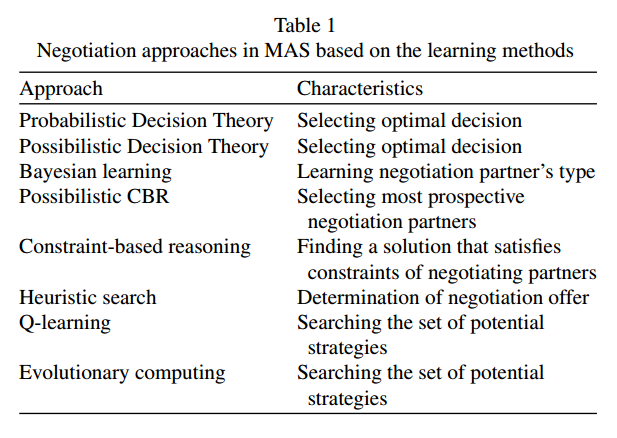
\includegraphics[width=0.7\linewidth]{img/negotiation_learning}
\caption{Overview of different learning methods for heuristic negotiation methods from \citet{beheshti2014homan}}
\label{fig:negotiationlearning}
\end{figure}
Based on the research conducted on heuristic methods and \citet{jennings2001automated}, it can be concluded that the optimal research in learning in heuristic methods is not yet known. They are often used however to decide on the optimal counter bid in \citet{beheshti2014homan}. They show that efficient learning algorithms based on an statistical ranking algorithm and linear regression, all with linear time complexities. These characteristics allow our method to be used in real-world applications. 
\section{Negotiation in Manufacturing}
There are many applications of agent based solutions in the manufacturing world \citep{monostori2006agent}. In these negotiations an overwhelming aspects is realised in the creation of intelligent individual agents, and less on the overall intelligence of the system. Often ignored is the specific negotiation method in these systems. This is where the problem lays, since conflicting interest, essential in the optimal decision making are left out. An example where these conflicting interest are well implemented is in \citet{zheng2014cloud}. A cloud consumer usually prefers a high reliability, whereas a cloud provider may only guarantee a less than maximum reliability in order to reduce costs and maximize profits. If such a conflict occurs, a Service Level Agreement cannot be reached without negotiation. Automated negotiation occurs, when software agents negotiate on behalf of their human counterparts. However no learning occurs. 

%Many negotiation solutions have been ``invented'' but little has been truly applied in the manufacturing world \citep{leitao2009agent}. 

Rockwell Automation uses agents in its automation processes and is one of the industrial leaders in the implementation of agent based solutions \citep{vrba2011rockwell}. One of their future insights in the requirements of agent based solutions is to enhance the capabilities of agents for expressing and exchanging knowledge, and as a consequence, to increase the flexibility of control systems. In order to correctly do so, better insights in the negotiation is needed.

Overall, nearly all factory scheduling negotiations use some form of these market-based approaches \citep{monostori2006agent} to implement the solutions. Different version of the contract net protocol were used or other auction based methods. The problem with these methods is that no reasoning about another's interest and desires is achievable. If this is known, more efficient and better systems can be achieved. It is however shown in \citet{bruccoleri2005production} that the agent based approach using market auctions out performs the centralized mixed integer programming solution. This system uses bilateral simultaneous negotiation on the medium level of the production plant. It is however a form of auctions, where the agents simultaneously bid towards the goal. If this system already outperforms a centralized system, a non-auction based method might outperform even better.

Other examples of negotiation in a Multi-Agent System have been deployed in Smart Grids for optimal energy delivery~\citep{pipattanasomporn2009multi}, the collaborative design of light industrial buildings~\citep{anumba2003negotiation}, negotiation in an electronic market of water rights, and for example in the scheduling of Agile software development~\citep{rabelo1999multi}. 

From the above, in comparison with the knowledge obtained, there are two gaps. Firstly, little multi-issue multi-lateral strategic (game theory wise) application have been implemented. An example from the theory is \citet{wu2009efficient} where a Pareto-optimal-search method for three-agent multilateral negotiation is developed. This however has not been implemented in any real usecase, and would be very interesting to implement. The other gap in the literature is the research into the optimal learning methods for heuristic methods. In \citet{de2015automated} a wireless surveillance sensor networks is optimized using heuristic learning methods. This is limited to a bilateral negotiation protocol with a mediator, where negotiating agents (two access providers, each of them controlling a fraction of the access points in the scenario) negotiate. No multilateral application has been attempted. An attempt at generalizing multilateral heuristic learning has been made in \citet{beheshti2014homan}, but this has not been applied to a real use case as of yet.

The last option, an application of multilateral heuristic learning, is the best fit on the usecase.
%So, in future, more concrete work should be done to validate more globally the decision-making support system and to find the most appropriated architecture ensuring “a form” of hierarchy (to optimise the global performances) and of co-operation (to be locally more reactive). It can lead (a) to evolve towards benchmarking, will not thus limit “to evaluate” only the protocol of negotiation we presented but also some of its derivatives and other types of negotiations, (b) to “automatise” the utility function of each expert (automated human expert) based on techniques such Bayesian Network, Fuzzy Logic,…to reduce the complexity of each decision (and to help the expert to develop his proposal), and (c) to use formal proofs to prove the global behaviour properties of the e-maintenance architecture (dynamics of the agent interaction and of the result emergence).  \cite{yu2003multi}

%In \cite{harjunkoski2009integration} it is stated that  Even if it is today technically possible to connect every single device within a control system into an plant-wide MES system, it would make very little sense to integrate these e.g. with the scheduling. This is due to traditional view of a centralized system for planning. What this fails to see is the positive effect it would have if 
% An Adaptive Negotiation Framework for Agent Based Dynamic Manufacturing Scheduling 
%Manufacturing scheduling problems, especially in a dynamic, uncertain environment, belong ta the NP-hard class. Agent based approach has been considered as a promising solution to these types of problems. However, it brings in another challenge which is how to make those costly negotiation processes among agents effective. This paper addresses this problem by proposing an Adaptive Negotiation Framework which models the dynamic nature of agent based manufacturing scheduling at negotiation level explicitly, The main contributions of this paper include: (I) an Agent-Based Adaptive Negotiation Framework for manufacturing scheduling, (2) selection heuristics of multiple economically inspired negotiation models, (3) the integration of adaptive negotiation heuristics, economic models and the coordinated Intelligent Rational agent architecture. 
%
%In the category of multi-agent systems (Bonabeau \& Theraulaz, 2000; Wooldridge, 2002; Brussel \& Wyns \& Valckenaers \& Bongaerts, 1998), ontology based optimizers were preferred ahead of generic particle swarm optimizers, as ontology based systems attempt to assess the consequence of mutation of the existing solution, prior to mutating, whilst generic PSO's mutate and then assess the fitness of the solution in the solution landscape. For practitioners this means that ontology based systems have fewer mutations though the run-time is comparable with PSO's. Finally amongst the different categories of ontology based systems, negotiating resource-demand-networks have shown to be most efficient (Rzevski \& Skobelev,2007; Skobelev, 2011; Multi-Agent Technology web-site (2012).
%
%An overview of agents in manufacturing is given by \citet{monostori2006agent}, where he gives an thorough and complete overview. In this paper a focus lies on the negotiation in a Multi-Agent solution, and thus the focus lies here as well. 
%
%\citep{shen2003multi}
%%\section{Artificial Intelligence}
%The research will be based on an intelligent Multi-Agent System (MAS) which would consist of sensors, connected as an Internet of Things (IoT) network. For the intelligent agents it would be possible, by understanding the system, and negotiating, to come up with the optimal inspection and maintenance schedule based on real-time data acquisition, analysis, negotiations and decentralized autonomous decision making. Such intelligence is an example of a typical MAS where artificial intelligence may include methodical, functional, procedural approach, algorithmic search and/or reinforcement learning. 
%%\subsection{Internet of Things}
%%
%% %%%%%%%%%%%%%%%%%%%%%%%%%%%%%%%%%%%%%%%%%%%%%5


%cite{anumba2003negotiation}
%Although there are essential differences between agent negotiations and human beings negotiations, the negotiation theories developed based on human activities are also the basis for agent negotiations. The adoption and development of negotiation mechanism depends on the application environment, requirements, and expectations of MAS.

%Game theory has a history of being applied to human or animal behaviour, but one of the main criticisms for the application of game theory has been that animals and, in particular, humans exhibit much more complicated behaviour than these simple models predict; human beings often do not act rationally and frequently do not have consistent preferences over alternatives. Machines, on the other hand, are governed by more consistent preferences, have generally very simple goals and motivations, and are more predictable. Game theory would seem to lend itself to use by intelligent agents and provides a basic negotiation mechanism for most MAS.

%However, there are problems. Much of the basic intelligent agent game theory research has been on ‘toy’ problems such as Blocks World, where a number of blocks placed in known slots, or on each other, have to be rearranged. In such problems the domain is small and all outcomes can easily be evaluated. Much of the theory is focussed on deriving conditions under which the most optimal deal is always reached. In the real world, these conditions can rarely be met and criticism has focussed on the many unrealistic assumptions of these approaches [27]. As a result, the axiomatic approaches are not suitable for the complex agent negotiation systems because they are basically static approaches, where the outcomes of the negotiation are emphasised.

%On the other hand, the strategic approaches, as a dynamic approach, overcome some of the major problems of the axiomatic approaches. Since the strategic approaches focus on the negotiation process as well as the outcomes of negotiations, such approaches are more suitable to the cases where the negotiation process is important. A typical example is the negotiations about the wage between the management group and the union. How one party makes a concession is important for another party to make their decision.

%Although the strategic approaches could be adopted for the design of agent negotiation mechanisms, many criticisms to the approaches are still very real when they are used to handle the real world problems. A major consideration is human responses during negotiation. Being more realistic and effective, behaviour models often provide interesting aspects for the development of agent negotiation mechanism. One of the examples is the learning mechanism which allows agents to get more realistic ideas about the opponent's negotiation strategy based on the opponent's offer during the negotiation process [51]. Some simple mechanisms such as the Bayesian rule allows intelligent agents to adopt such a learning ability. Beside learning mechanism, other behaviour models such as the dual response model and the joint decision making model are also applicable to building a sophisticated negotiation mechanism for MAS.

%Besides choosing the key negotiation approaches, there are many other factors that need to be addressed based on the application scenario. Kraus [20] explains that there are five issues which need to be further determined if game theory is selected as the basic negotiation mechanism. They are: choosing a strategic bargaining model which is applicable to the problem; matching the scenarios with the game-theoretic definitions of the chosen model; identifying equilibrium strategies; developing low complexity techniques for searching for appropriate strategies; and providing utility functions.



%approximate-optimale oplossingen terwijl je de optimale oplossing niet weet lijkt een leuke uitdaging
\section{Framework of a centralized and decentralized system}
When looking at the traditional pyramid, which is fully centralized, it seems difficult, if not impossible to translate this to a decentralized solution as shown in \Cref{lit:manufacture}. It should be possible to determine whether a centralized or decentralized solution, using a MAS or holonic system, should be implemented at a business process. A framework to compare a centralized versus a decentralised solution is discussed here. Essential in the difference between these two possible solution spaces is the location of the processing power for the calculations. Centralised solutions have a single control unit where the information flows to, while decentralized solutions do not have this structure.

A popular comparison, discussed by \citet{parunak1999industrial}, is that of the original Roman army structures. Decisions where made at the top and dripped down, while the information stream went up. This method has been deployed in most companies. Due to the fact that something can be computed on a single computer, and be optimized on this single program, an optimal decision can be found.

However, the increasing complexity of computer and information systems, combined with the increasing complexity of their applications, exceed the level of conventional centralized computing. This is due to the processing of huge amounts of data, or data that originate from different locations. To solve such difficulties, computers have to act more like agents where each agent can solve, or decide on part of the problem. This is where agent-based architectures are an ideal fit to such a decentralized organizational structure.

To push the decision making to the lowest level, excessive layers of management can be obsolete. This allows for, sometimes, easier to understand and developing of problems, especially if the problem being solved is itself distributed.

By using principles of decomposition which is a classical optimization (reformulation) method \citep{sharif2012yard} presents a comparative study of two contrasting approaches for modelling the yard crane scheduling problem: centralized and decentralized. It seeks to assess their relative performances and factors that affect their performances. They conclude that a centralized approach outperforms the decentralized approach by 16.5 \% on average, due to having complete and accurate information about future truck arrivals. However, since the decentralized under performs the centralized, the decentralized approach can dynamically adapt to real-time dynamic changes, making it better suited for real-life operations. 

To optimize these different types of resources allocation problems, there are different kinds of allocation problems, for which different solutions are feasible. The purpose here is to find what characteristics are optimal to use a centralized vs a decentralized solution.


\subsection{Size and Modularity}
A critical aspect of the possibility to determine whether a centralized or decentralised solutions is preferred is the search space size of the problem. The size of the problem is seen as the number of resources or task that have to be allocated.  If a clear structure is conceivable and a clear population is in place a centralized solution is infeasible. This is due to the global overview. However, the high sensitivity to size and complexity makes a centralized solution impracticable.

In a decentralized structure, individual models are decoupled from one another, errors in one module impact only those modules that interact with it, leaving the rest of the system unaffected. This can be seen in \Cref{fig:modularitydecentral-changeability}. It shows however the importance of having a clear modular problem. 

\begin{figure}[h]
\centering
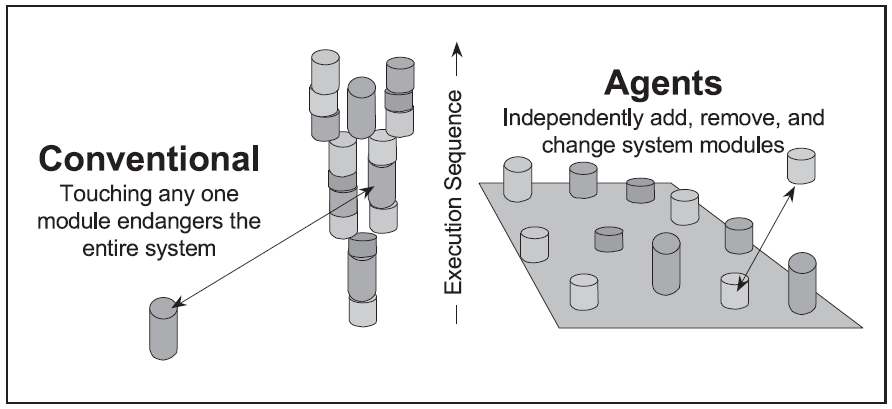
\includegraphics[width=0.7\linewidth]{img/modularity+decentral-changeability}
\caption{Comparison of a conventional control thread and an agent-based control, from \citep{parunak1999industrial}.}
\label{fig:modularitydecentral-changeability}
\end{figure}



\subsection{Dynamicity (Time Scale/Changeability)}
In a decentralized solution, the continuous monitoring of the state of the environment and typically the lack of complex decisions, a quick reaction to changes is possible. A high dynamical is the result. 

Unfortunately, it is difficult to achieve real-time scheduling in traditional manufacturing systems because the scheduling algorithms used are executed on a single, centralized computer that becomes computational incredibly difficult \citep{duffie1994real}.
\subsection{Solution Quality}
Since agent-based approaches are distributed, they do not have a global view of the entire state of a system. A lot can reached through communication and negotiation, but for a truly optimal solution, an entire view is necessary For example,  \citep{palmer2003decentralized} shows that this algorithm is not intended to find the optimal solution; it finds a good solution with less computation. 

In the centralized approach the assumption of a complete information on supply and demand is made. This requires rescheduling to adapt with changes. In the decentralized approach, no assumptions on the complete information is necessary. 


\subsection{Complexity}
Since an agent can execute actions only on its own surrounding, it is dependent on its local parameters. However, the agent can use information sent by its neighbours to adapt \citep{pujolle2006autonomic}. This interaction between the elements makes the complexity of a solution many times higher and more difficult than a centralized solution.

\subsection{Framework Overview}
Below a summary of the points above is given, with respect to the structure given. It is obvious that a decentralized solution is preferred, if the problem can be divided into sub problems. However, the real difficulty then lies in the complexity. Since in the system the communication becomes essential, the complexity increases.

\begin{tabular}{p{1.5cm} p{2.5cm} p{2.5cm} p{2.7cm}}
	\toprule
	& Centralised Solution & Decentralised Solution & Building Blocks\\
	\midrule
	Size / Modularity & Small; No sub-problems & Large; Ill-Structured; Easily dividable; Independent Modules & Population; Holonic; number of resources: (decision variables, parameters \& constraints) \citep{lang2015collaborative} \\
		\midrule
	Time scale and Changeability & Days - Weeks; Not subject to a lot of change & Real-time - Hour; Changeable  & Adaptive Capability ; Degree of Re- and Pro-activeness \citep{parunak1999industrial} \\
	\midrule
	Solution quality & Perfect & (sub-)Optimal & Object and Solution Space \citep{sharif2012yard} \\
	\midrule
	Complexity & Simple & Complex & Interaction between the set of elements; Communication \citep{pujolle2006autonomic} \\
	
	\bottomrule
\end{tabular}


\section*{Negotiation in a Decentralized Structure}
By decomposing the problem in smaller sub problems that a single agent can compute, and solve, the communication of the agents is essential. In order to integrate the solutions of the sub problems into the overall solution, the agents, which might not be cooperative, need to use negotiation.
%To achieve the autonomic-oriented architecture, we propose to select the appropriate control mechanisms among: 
%- adaptive: the agent adapts its actions according to the incoming events and to its vision of the current system state. The approach we propose is adaptive as the agent adapts the current control mechanisms and the actions undertaken when a certain event occurs. The actions the control mechanism executes may become no longer valid and must therefore be replaced by other actions. These new actions are indeed more suitable to the current observed state;
%- distribution: each agent is responsible for a local control. There is no centralization of the information collected by the different agents, and the decisions the agent performs are in no way based on global parameters. This feature is very important as this avoids having bottlenecks around a central control entity;
%- local: the agent executes actions on the elements of the node it belongs to. These actions depend on local parameters. However, the agent can use information sent by its neighbours to adapt the activated control mechanisms;
%- scalable: the proposed approach is scalable because it is based on a multi-agent system which scales well with the growing size of the controlled network. In order to adaptively control a new node, one has to integrate an agent (or a group of agents) in this node to perform the control. 

\chapter{Research Design \& Application}
\label{ch:design}
As discussed in the literature review (\Cref{ch:literature}), this research has a focus on the negotiation of agents. Using different methods and techniques, an attempt is made to optimize a production process. The agents attempt to find an approximate-optimal solution while the optimal solution is unknown to the group. %Based on learning methods from decentralized holonistic methods, utility and negotation domains a simulation can be build which can be applied to the production process. 

The system in which the  decentralized solution will be applied is a de-mineralized water plant as described in the introduction and problem chapters (\Cref{ch:intro}).

As explained in the literature, a negotiation problem can be characterized by a negotiation domain (who negotiate and what do they negotiate about), an interaction protocol (which rules govern the negotiation process) and a set of decision mechanisms or strategies that guide the negotiating agents through every phase of the interaction protocol \citep{fatima2014principles}.

For the scope of this work, we assume a multi-attribute negotiation domain, where a deal or solution to the problem is defined as the set of attributes (issues), and each one of them can be in a certain range.

The coding will be done in Java from scratch. Multiple open-source systems are available, including Jadex, which is perfect for communication research in a Multi-Agent System \citep{kravari2015survey}. However, since most of these systems are very comprehensive, little adjustments which are necessary for our research are not conceivable. Secondly,  specific requirements, with the projections for example were to new, for old methods. 

%\section{Mapping of Literature on usecase}
%	\begin{tabular}{p{2cm}|p{2cm}|p{2cm} l l |p{3cm}}
%		& Category & Literature & & & Usecase\\
%		\hline \hline
%		Real-time & Physical (process) & Object/service oriented programming & & & Operations:
%		\begin{itemize} 	
%			\item Production Guarantee (leveringszekerheid) 
%			\item Batch Production 
%			\item Ions, flow, Ammonia (water softening)		
%		\end{itemize}\\
%		\hline
%		Real-time & Sensing & Programmable Logic Controller; Real-time Monitor & \multirow{2}{*}{\rotatebox[origin=c]{90}{Holonic, Cyber-Physical}} & %\multirow{3}{*}{\rotatebox[origin=c]{90}{e-manufacturing}}
%		& Sensors (mineral, temperature, softening, ammonia, flow)\\
%		\hline
%		Sec - Min & Analysis & Agent; BDI; Data Analysis; Machine Learning & & & Predictive/Condition based Maintenance\\
%		\hline
%		Hours - Weeks & Work order/Action & Planning; MAS; Scheduling; Game Theory & \multirow{2}{*}{\rotatebox{90}{Negotiation}}& & Work flow; Logisics Spare Parts; Process control feedback; integrated supply chain
%		
%	\end{tabular}
%\section{Mapping of Negotiation}
%
%As can be seen, negotiation is in the two highest. We focus on this.
%\todo[uitleggen negotiation]{uitleggen negotiation}

\section{Demineralization of water}
As discussed in the introduction, the usecase for which a Multi-Agent system for production will be implemented is a water demineralization plant. An application of this new model will be applied to a large plant that creates de-mineralized water. By removing all the ions from common water, de-mineralized water is obtained. This water is used for many processes and has many applications. In this plant specifically, it is used for the steam turbines, which generate electricity. By burning the by-product, heat is generated, which creates steam to power the turbines. 

\begin{figure}[h]
	\centering
	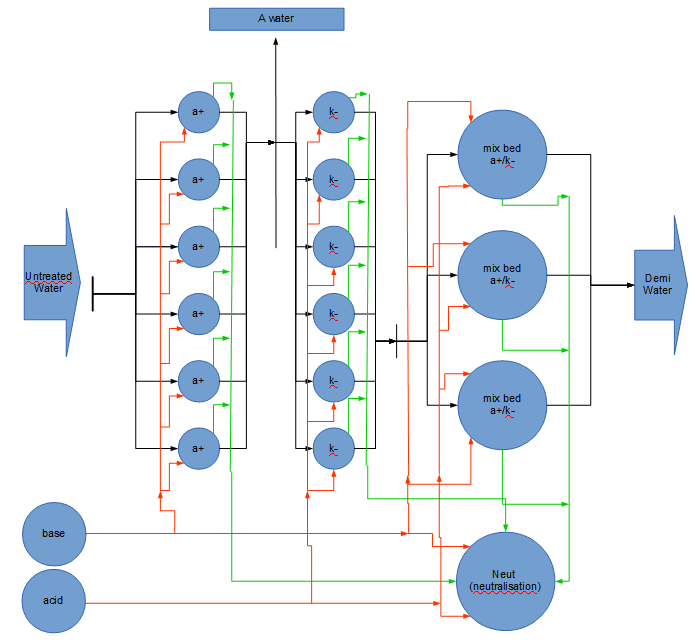
\includegraphics[width=1\linewidth]{img/demi-plant}
	\caption{An overview of a water demineralization plant. We simplify the many anion and cation filters to a single anion and cation filter. The same for the Mixbed filter.}
	\label{fig:demi-plant}
\end{figure}

Minerals are removed from water by multiple production steps. The most common method, which is implemented in the plant described, is to first remove the positively charged minerals in so-called anions. After this the negative charged ions are removed within a cation filter. To ensure that all ions are removed, a final combined ``Mixbed'' is used. Here a combination of an anion filter and a cation filter removes the residues.

These filters have to be cleaned every few hours to ensure that proper demineralization occurs. For cleaning, acid and base are used. By filtering the anion with base, the ions that have been retrieved in the filtering are flushed. The residue, still of a base composition, is stored in a storage tank where the combination of the base and acids from the filters is neutralized. This storage tank is called the ``Neut'' as short.

So overall, we have three kinds of filters, the anions, the cations, the Mixbed and the residue storage tank: the Neut. Each of the filters is exemplified by multiple items, but for simplification we only look at the allocation of resources. So overall there are 4 agents: 1. ``Anion'', 2. ``Cation'', 3. ``Mixbed'', 4. ``Neut''. Within each agent, the right amount of resources will be allocated. This will be done by negotiation and combined with the information that is retrieved from the experts knowledge.


\section{Negotiation model}
\label{sec:design:negmod}
These four rational agents, $m = \{1,2,3, 4\}$, partition three issues $n=\{1,2,3\}$: 1. the acid that is needed for cleaning, 2. the base for cleaning, 3. the water that has to be delivered at the end of the process. This can be simplified to a multilateral buyer-seller negotiation.

Anion wants as much base as possible, while it wants to minimize the amount of water. For the cation, as much acid as possible is required, while still as little water as possible should be produced. The Mixbed requires as much as possible acid and base for cleaning. Since it the final production step, it requires the water to be delivered, forcing it to obtain as much water as possible from the cation. Finally there is the Neut, which wants as little base and acid as possible. Also the base and acid should be levelled out as much as possible to attempt to stay as close to a pH of $7$ as possible. 

Each of the above issues is translated to a unit interval $[0, 1]$ in $\mathbb{R}$. Since we have $3$ issues, the unit hypercube $[0, 1]^3$ in  $\mathbb{R}^3$. This results in a possible negotiation domain $\Omega = [0,1]$ per issue.

The utility function for each agent $u_i(x)$ is convex, as described in \Cref{sec:convex}, and normalized between $[0, 1]^3$. Each agent has a reservation utility $ru_i$. Any offer below this reservation utility is unacceptable. This means that the set of feasible offers, or the agreement-zone, is $A = \{ x\in [0,1]^3 \mid u_i(x)\geq ru_i\}$. Since the function is convex, $A$ is also convex. The solution, if it exists, lies in the intersection of feasible offers, $\mathbb{Z} \cap^M_{i=1}A^i$.

The protocol used is that of the alternating offers protocol, based on \citep{rubinstein1982perfect} as described in \Cref{sec:negotiation}. The agents will propose in a fixed sequence, where the new offer is based on all previous offers given in the previous round. If all agents accept a current offer, the negotiation ends. The overall protocol is based on \citep{zheng2015automated}. 
	%The protocol is based on the method as proposed by \citet{wu2009efficient}. Here an multilateral multi-issue method for negotiation about the allocation of resources is given. 

%Since the agents have no knowledge regarding the states of the other agents, 
It is a difficult task to determine whether the solution is a proper one, since the agents only have knowledge of their own utility function, which is private. 

The negotiation takes place in rounds $n\in \mathbb{N} $. ${x}_i \in [0,1]^3$ denotes a bid of agent $i \in m$ in a round and $x_{j}\in {x}_i$  denote the amount of issue $j \in n$. 

%Using BDI in each agent, the anion will know which filter to use when, and when to clean them. This intelligence can be learned. There is a limit on the amount of water, base or acid.

%Head tries to increase the holon utility as a whole, and this does not contradict the increase in body-agent utility. In other words, Head wants to increase holon’s utility, and is willing to do this according to body-agent preference. 

\begin{figure}
	\centering
	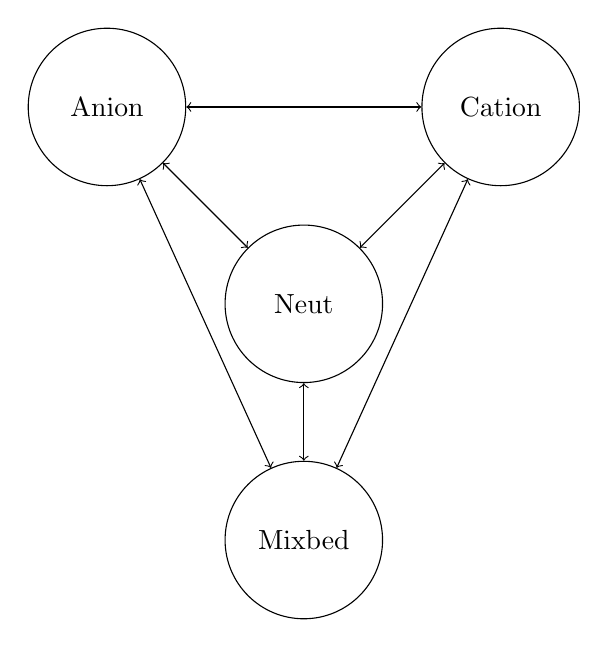
\begin{tikzpicture}
	\node[circle,draw, minimum size=2cm] (A) at  (0,0) {Neut};
	\node[circle,draw, minimum size=2cm] (B) at (-2.5,2.5) {Anion};
	\node[circle,draw, minimum size=2cm] (C) at (2.5,2.5) {Cation};
	\node[circle,draw, minimum size=2cm] (D) at (0,-3) {Mixbed};
	
	\draw[<->] (A) -- (B);
	\draw[<->] (A) -- (C);
	\draw[<->] (A) -- (D);
	\draw[<->] (B) -- (C);
	\draw[<->] (B) -- (D);
	\draw[<->] (C) -- (D);
	\end{tikzpicture}
	\caption{A simplified representation of the agents in the negotiation. See \Cref{fig:demi-plant} for the overview of the water plant on which the model is based.}
	\label{fig:agent-plant}
\end{figure}

\section{Details of the Agents}
Each agent has its own characteristics on which the system will run. As shown in the introduction, the agents have difference preferences regarding the allocation of the resources. An offer has a different utility for each agent. 

When the negotiations start, each agent will attempt to obtain as much utility as possible. Thus, when negotiations start, they propose the offer with the highest utility for them. During the negotiation, the required utility slowly decreases. An agent $i$'s concession strategy is defined as a time series of the agent's desirable utility at time $0,1,...,t$. This is written as $s_i(0), s_i(1), s_i(2),..., s_i(t)$.  This is a monotonically decreasing function of the time/rounds $t$. The concession strategy $s$, is agent dependent. However, this utility will always be larger than the agent's minimum utility, or reservation curve: $s_i(t) \geq ru_i, \forall t$.

Since the utility decreases each round, the set of feasible offers increases as well. This means that at time $t$, agent $i$ has the convex set $A^i_t = \{x\in [0,1]^3 \mid u_i(x) \geq s_i(t)   \}$ as possible offers. Since $s_i(t)$ is monotonically decreasing, this means that $\forall t, A^i_1\subseteq A^i_2 \subseteq ... \subseteq A^i$. In this model, we use the amount of utility monotonic concession protocol as described in \Cref{sec:concessionstrat}, since it performs well, and has the advantage of finding a solution in a specific time.

\subsection{Reactive concession strategy}
\label{sec:reactiveconcessionstr}
The reactive concession protocol as described by \citet{zheng2015automated}, and also shown in \Cref{sec:concessionstrat}, is a specific concession strategy to determine the amount of utility to concede. The non-reactive concession follows a predefined concession strategy $s_i^0(1), s_i^0(2),...,s_i^0(T)$, where $T$ is the maximum amount of rounds. The reactive concession, ($s_i(1), s_i(2),..., s_i(T)$), amount is determined by each agent by the utility change resulting from other agents' offers. The nonreactive concession made at time $t$ is $\Delta u_{i0} = s^0_i(1)-s^0_i(t-1)$.

There are two options for an agent to concede. Either the change in utility that the other agents' caused is above the reservation function. In this case, an agent does a concession according to the non-reactive concession strategy as calculated above. 


 However, if the change is below the reservation function the agents concedes by an amount based on the change the agent perceives in its own utility. This is shown in \Cref{al:algorithm1},  \Cref{al:start} to \Cref{al:end}.
 
 The perceived change of utility for agent $i$ from agent $j$ is defined as the difference between the utility of the current offer and that of the previous best offer: $u_i(x^j_t)-u_i(x^j_{[,-1]})$.
 
 The total perceived change since the beginning of negotiation is equal tot the difference between the utility of the current offer and that of the first offer: $u_i(x^j_t)-u_i(x^j_0)$. Since we only want to concede compared to our own concessions, we subtract this perceived change from our change: $(1-u_i(x^i(t-1))$.
 
 The maximum of these function is the amount the agent is willing to concede per agent: $\max \{\Delta_1u_{jk}(t), \Delta_2u_{jk}(t),0\}$

This value is determined for each agent, whom then takes the minimum amount of all these values, to determine its concession $\min \{\displaystyle \min_{k\in 1, 2, 3, 4}\Delta u_{jk}(t), \Delta u_{j0}(t)\}$.

The convex requirement makes it obvious why the reactive concession can be used. If a non-convex utility function was to be used, it could not have been determined whether an agent concedes if it moves. 



\subsubsection{Offer generation}
When an agent $j$ has offered $x_j\in[0,1]^3$, the next agent $i$ will either accept the offer $x^j_t$, or create a new offer $x^j_{t+1}$. 

To create the new offer, the agent $i$ will first calculate the weight of all the offers by other agents ($j$). This is done by $\sum_{j=1}^{m} a^{i,j}_t x^j_t $ where $\sum_{j=1}^{m}a^{i,j}_t = 1$. For simplicity, we set the $a^{i,j}_t = \frac{1}{m} = \frac{1}{4}$. 
This weighted average of the offers is projected by on the border of its feasible offer set $A^i_t$, thus we get $x^j_{t+1}$. This boundary, or indifference curve, is the set of points for which the utility is equal to the desired utility of agent $j$. The projection can be done using convex projection techniques as explained by \citet{boyd2004convex}. In this method, a linear indifference curve will always be obtained, making convex projection calculations unnecessary. This will be done to ensure a high speed run-time, since the state of the world will change quickly.


%The basis consists of the different sub agents. The head agent will know the state of the sub agents and will negotation on heave of the entire group. 

%Important to note is that the utility function is required to be convex. 
\subsection{Anion}
The anion is the first filter where the untreated water will arrive. It needs base to clean the filters after water has been produced. The water that is produced by the anion filter will flow to the cation filter. The anion and cation filter both have a low interest in the production of water, and thus do not need to negotiate which each other.%The filters have different characteristics and it is the job of the head to decide on the filters task. Some will be paused, some will filter, and others will be cleaned. 

\begin{figure}[h]
	\centering
	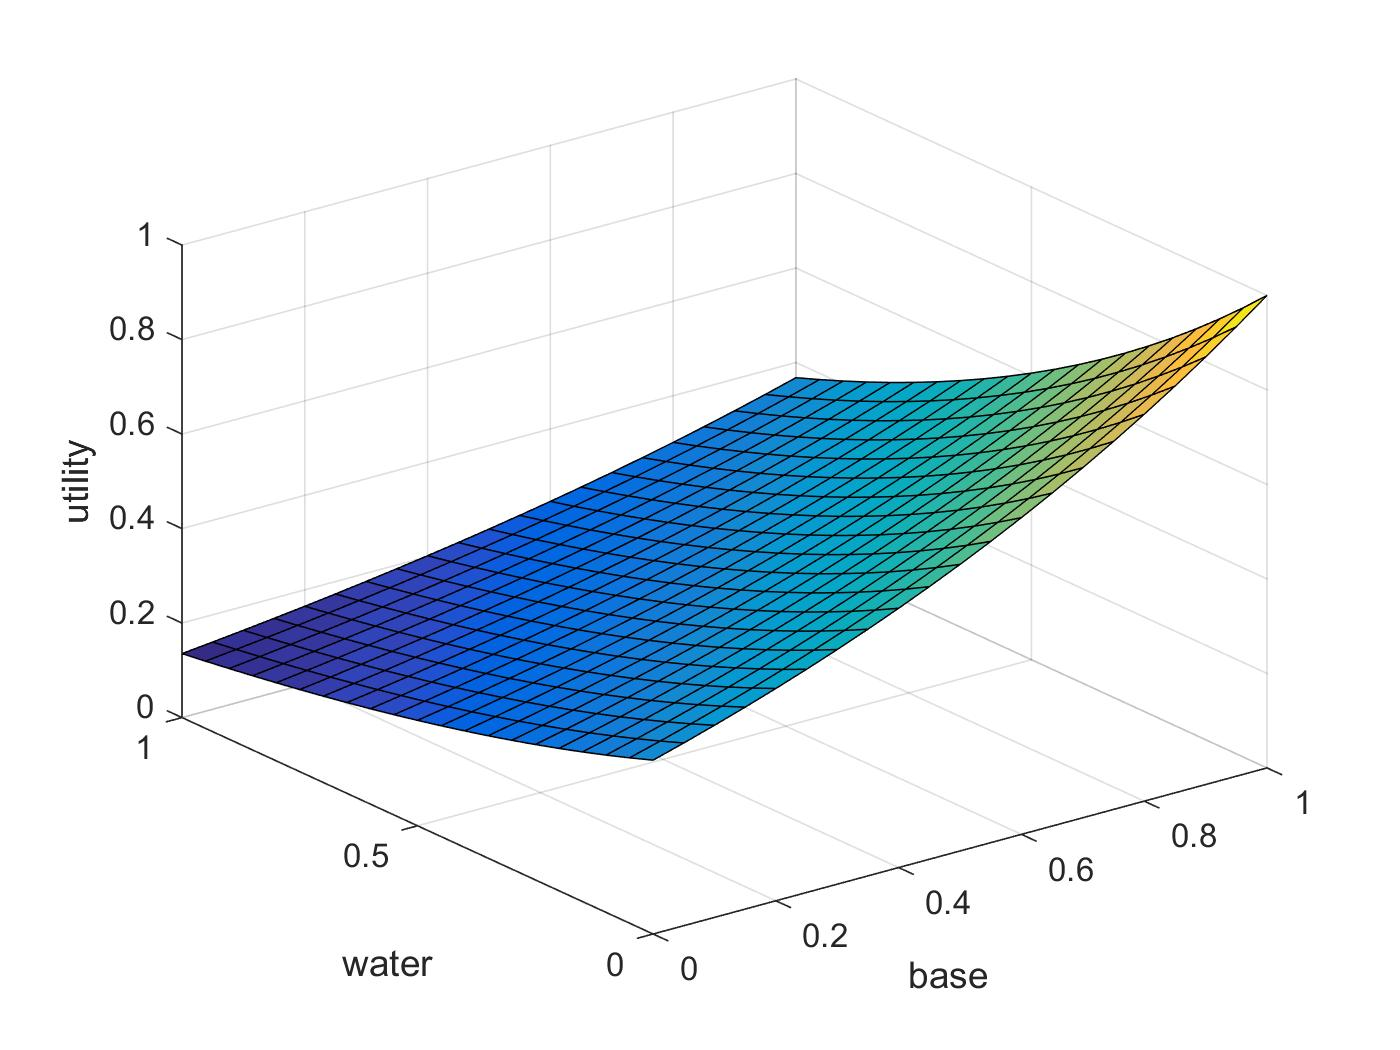
\includegraphics[width=0.7\linewidth]{img/Anion_utility}
	\caption{The utility function for the Anion.}
	\label{fig:anionutility}
\end{figure}

\subsubsection{Utility function}
%As described in \citet{wong2010multi}, it is possible by combining the input into the utiltiy function of the agent. This is shown in \Cref{fig:wongutiltiyneuralnetwork}. 
The utility function for the anion filter is set up as follows:

\[
\text{Anion utility} = \frac{e^{-W+B}}{e^1}
\]
where W is water ranging over ([0,1]) and B is base ranging over([0,1]). The division by $e$ is done to ensure normalization. The utility is in [0,1]. It is visualized in \Cref{fig:anionutility}.

This function has been obtained after talks with industry experts. They confirmed that a high base wish, and low water wish is in line with the anion's utility. A consequence of this function is that it can be expressed as $ (\ln(u)+1) = -W+B$. This means that if the required utility is known, an indifference line is the result, as visualized in \Cref{fig:anionutilitycontour}.

\begin{figure}[h]
	\centering
	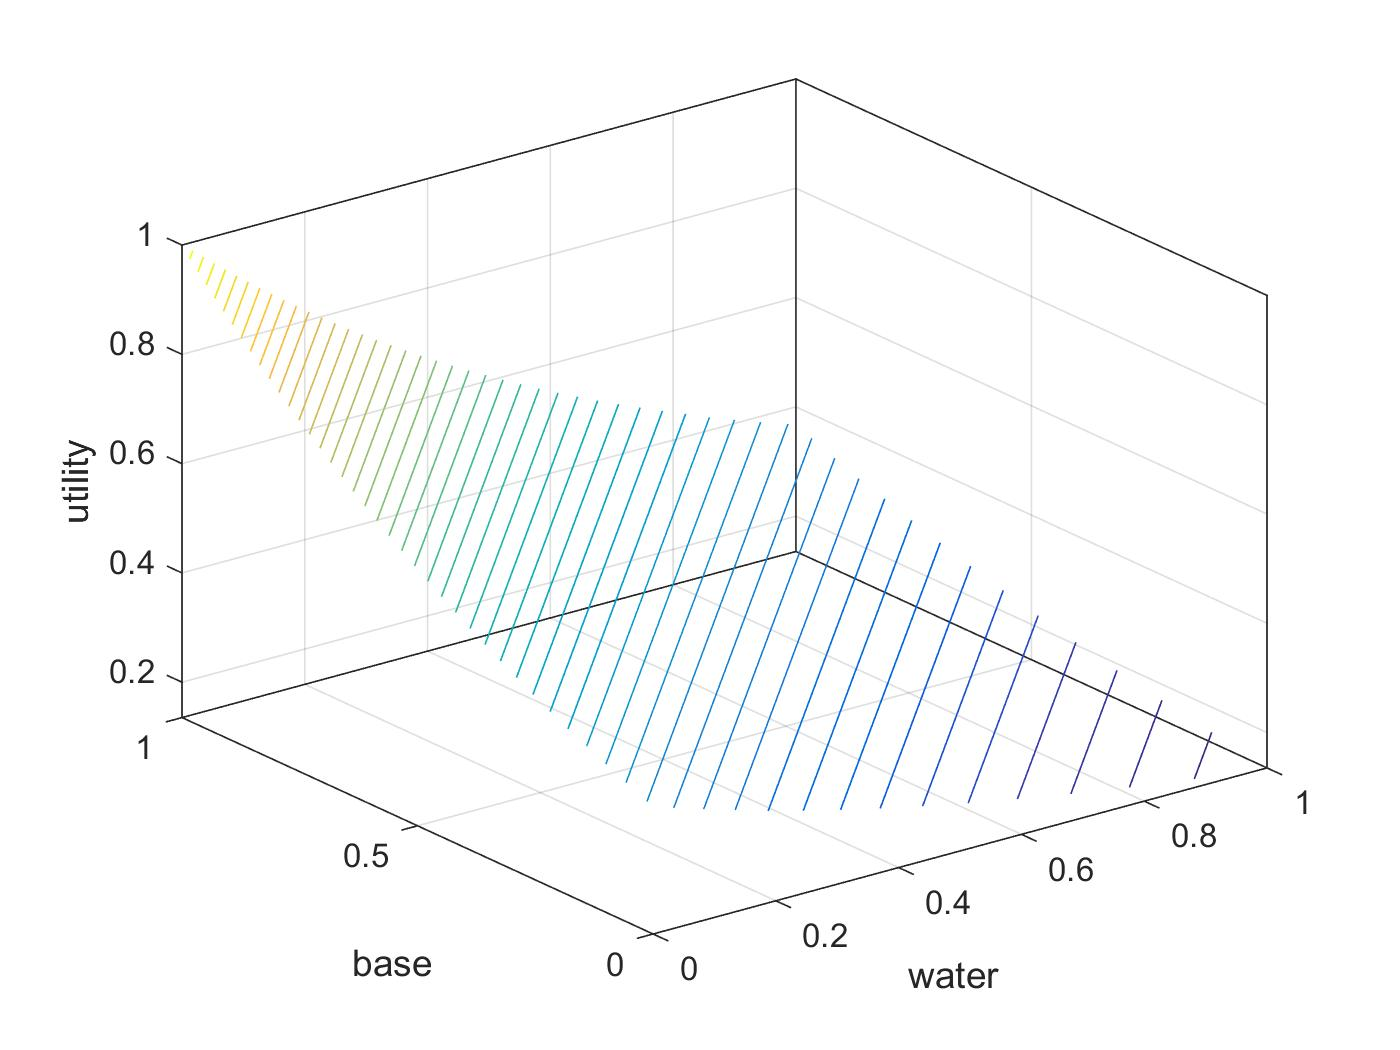
\includegraphics[width=0.7\linewidth]{img/Anion_utility_contour}
	\caption{The visualization of the indifference curves for the Anion agent.}
	\label{fig:anionutilitycontour}
\end{figure}

The reservation curve can be set as the curve where the utility $= 0.3$ e.g.. This means that any offer on the line $0 = B - W - (\ln(0.3)+1)$, or above, is acceptable for the anion in the stages of negotiation.

%At first a simple linear utiltiy function will be used: the less water, the higher the utility. Also, the more base, the higher the utility. This has a limit, depending on the reservation function as shown in \Cref{fig:anionreservationfunction}.

If the indifference line is know, a projection on this line is possible. 
At $t$, the agent $i$ (anion) has the required utility $s^i_t$. Suppose $s^i_t = 0.4$ This means that there is an indifference curve $0 = B - W - (\ln(0.4)+1)$. Suppose that offer $x(t-1)$ contains an offer for base $0.4 \text{ and water } 0.7$ (we can disregard the acid offer in this example, since the Anion has an indifference for the amount of acid used). 

A projection to the indifference curve of the Anion is achieved with the following formulae. It has been thoroughly proven that if function is written as, $\texttt{a} x + \texttt{b} y + \texttt{c} = 0$,the distance is calculated as follows:

\[\text{distance}(ax+by+c=0, (x_0, y_0)) = \frac{|ax_0+by_0+c|}{\sqrt{a^2+b^2}}. \]

From this we get the point of the line, which is the line with the minimal distance:
\[x = \frac{b(bx_0 - ay_0)-ac}{a^2 + b^2} \text{ and } y = \frac{a(-bx_0 + ay_0) - bc}{a^2+b^2}\]

This has been proven multiple times, for example by algebaric proof by finding the line that is perpendicular to the original line, and $b/-a$ (the negative reciprocal) by letting it pass trough the point ($x_0, y_0$). Then it is obvious that the distance is indeed as shown above, with the minimal distance point $x \text{ and }y$.

The above is important since \citet{zheng2015automated} has proven that if the projection is the point with the shortest minimum Eucilidean distance, the algorithm will converge for any concession strategy.

So given the situation above, we have the function $\texttt{a} x + \texttt{b} y + \texttt{c} = 0$ where $\texttt{a} = 1, \texttt{b} = -1, \texttt{c} = -(\ln(0.4)+1)$. Given the information above, $x_0 = 0.4 \text{ and } y_0 = 0.7$ this gives us the solution of the new $x=\frac{2.1 + \ln(0.4)}{2} \text{and} y = \frac{2.1 - \ln(0.4)}{2}$, which is on the indifference curve of the anion for an utility of 0.4.
The above is visualized in \Cref{fig:projectionanionexample}.

\begin{figure}[h]
	\centering
	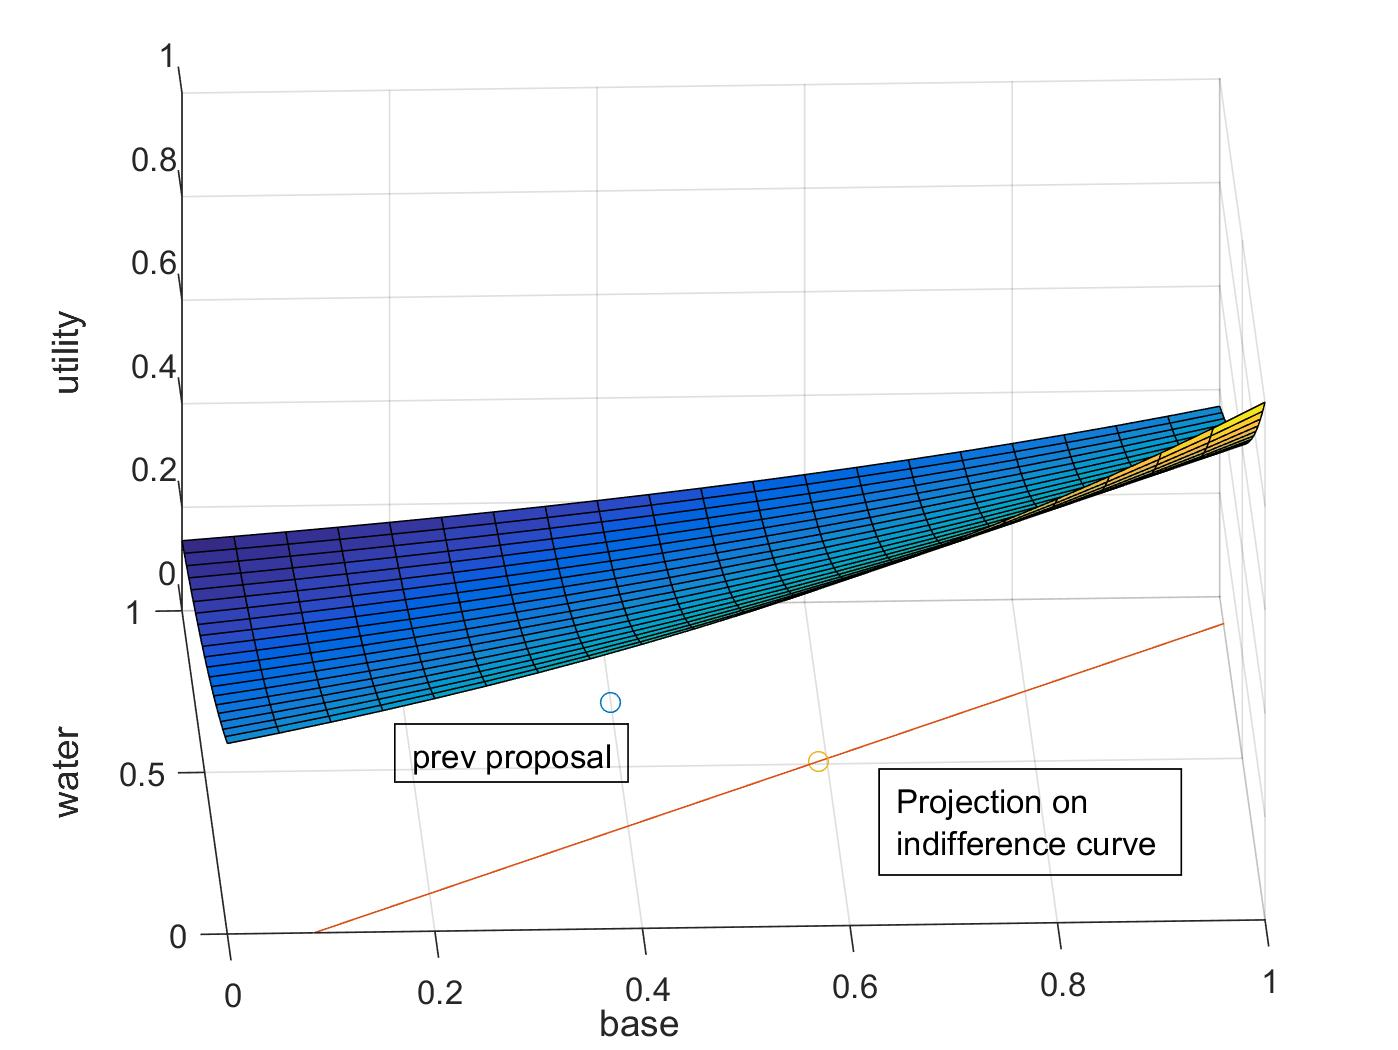
\includegraphics[width=0.7\linewidth]{img/projection_anion_example}
	\caption{Example of the projection of a point to the indifference curve for an Anion. The utility here is 0.4, and the offer is base = 0.4; water = 0.7.}
	\label{fig:projectionanionexample}
\end{figure}

The projection is formally written as $P_A[x]$, which is the projection of point $x$ on set $A$. 

Important to note is that if the utility of the new point is larger that the desired utility, (the point is above the indifference curve), the proposal will not be accepted.

The advantage of using a linear indifference curve is that we don't have to deal with an minimization function ($P_A[x] = \arg \displaystyle \min_{\forall q \in A} ||q-x||$) which increases speed dramatically.

If a point is projected outside the [0,1] boundary, the intersect of the indifference curve and the boundary is the closest point.






%\begin{figure}
%	\centering
%	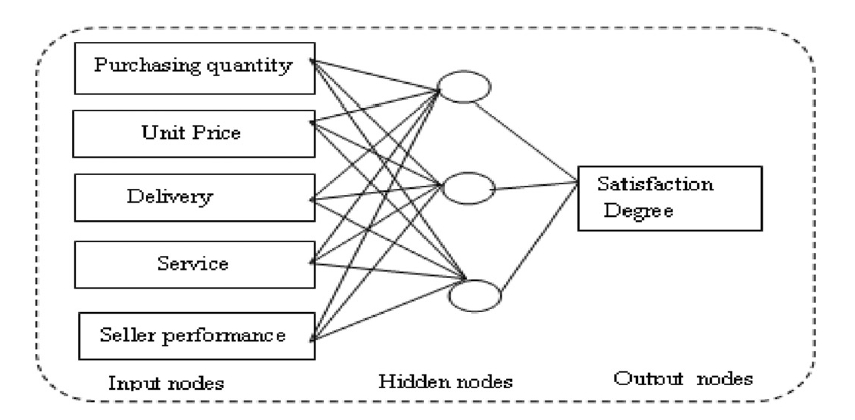
\includegraphics[width=0.7\linewidth]{img/wong_utiltiy_NeuralNetwork}
%	\caption{An example where the utility function is modelled with a Neural Network. \citep{wong2010multi}.}
%	\label{fig:wongutiltiyneuralnetwork}
%\end{figure}



%A very important input to the utility function is that of the belief in the other agents. These will not be formally modelled, as in Kripke worlds e.g., but can still be used as input to the utility function. 

\subsection{Cation}
The cation is the second aspect of the water cleaning process and is the siode where the positively charged ions are removed. It cleans itself with acid. %A overview of the filter is shown in \Cref{fig:cation-head-sub}.

The utility is very similar to that of the Anion, but a preference over acid instead of base is required. This results in the function:
\[
\text{Cation utility} = \frac{e^{-W+A}}{e^1}
\] 
where W is water ranging over ([0,1]) and A is acid ranging over ([0,1]).

The reservation curve for the Cation is very similar to that of the Anion. The only difference lies in the requirement for acid instead of base. It can been set as the curve where the utility $= 0.3$. This means that any offer on the line $0 = B - W - (\ln(0.3)+1)$, or above, is acceptable for the cation.

\subsection{Neut}
The Neut is the agent responsible for the allocation of the amount of acid and base. Since it wants to stay as pH-neutral as possible, it requires an even distribution of base and acid between the agents. This is not achieved in the utility function which is the same as the others, just different variables.

\[
\text{Neut utility} = \frac{e^{-A-B}}{e^3}
\] 
where B is base ranging over ([0,1]) and A is acid ranging over ([0,1]).

The reservation curve, however, is a little different. It consists of two functions, namely $0 \geq -B - A - 0.2 \text{ and }  0 \leq -B - A + 0.2$. The value of $0.2$ has been decided on after talks with experts. 

\begin{figure}[h]
		\centering
	      \begin{tikzpicture}
	      
	      [domain = 0.1:3.9]
	      
	      \draw[->] (0.02,0) -- (4.2,0) node[right] {$Base$}; 
	      \draw[->] (0,0.02) -- (0,4.2) node[left] {$Acid$};
	      \draw[scale=0.5,domain=0:6,smooth,variable=\x,black] plot ({\x},{\x+2}) node[left] {$ru^1_{Neut}$};
	      
	      \draw[scale=0.5,domain=2:8,smooth,variable=\x,black] plot ({\x},{\x-2}) node[right] {$ru^2_{Neut}$} ;
	      
	      \end{tikzpicture}
			\caption{The neut reservation curve of the Neut. The requirement of the acid and base staying near each other is achieved.}
			\label{fig:neutreservationcurve}
	\end{figure}
\clearpage
\subsection{Mixbed}

The Mixbed is where the final cleaning occurs. It is also the agent responsible for the end water delivery. Since it consists of a mixture of anion and base, it has three issues about it has desires. This is realized with the function below:
\[
\text{Mixbed utility} = \frac{e^{W+A+B}}{e^3}
\] 
where W is water ranging over ([0,1]), B is base ranging over ([0,1]) and A is acid ranging over([0,1]).

The reservation curve is given as $0 = A+B+W - (\ln(u)+3)  $. The projection of a point to this linear plane is calculated as follows:
\[
x = \frac{x_0 + (\ln(u)+3) - (x_0, y_0, z_0)}{3}
\]

\[
y = \frac{y_0 + (\ln(u)+3) - (x_0, y_0, z_0)}{3} 
\]

\[
z = \frac{z_0 + (\ln(u)+3) - (x_0, y_0, z_0)}{3}
\]

The shortest distance from a point to a plane is along a line perpendicular to the plane. By calculating the normal vector, which is perpendicular to the plane, we find the line that is parallel to the normal vectore, and goes through point ($x_0, y_0, z_0$). 

Important to note her is that the ratio of water to the base and acid is disputed. Since only a residue of ions have to be removed, the amount of water desired can be much hire compared to the amount of acid and base used. This is solved with the introduction of a variable $l$ with which to multiply the amount of water. 

If the amount of water, compared to the amount of base and acid used is 10 i.e., we get the following function:
 \[
 \text{Mixbed utility} = \frac{e^{(10*W)+A+B}}{e^(10+2)}
 \] 
The normalisation is still required, which is carried over to the projection to the plane in $x$ for example:
\[
x = \frac{x_0 + (\ln(u)+12) - (x_0, y_0, z_0)}{12}
\]
%These are shown in \Cref{fig:mixreservationfunction1, fig:mixreservationfunction2}.
\section{Negotiations among the agents}
All in all, there are three kinds of sub-negotiations. These are shown in \Cref{fig:agent-plant-base,,fig:agent-plant-acid,,fig:agent-plant-water}.

\begin{figure}[h]
	\centering
	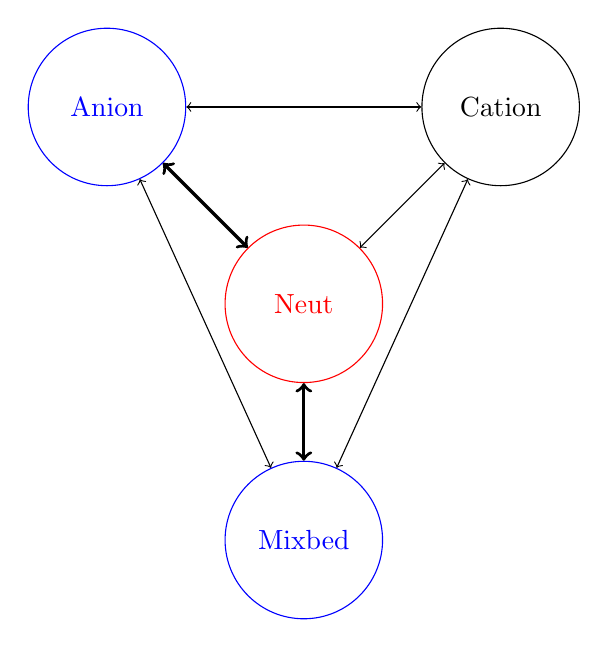
\begin{tikzpicture}
	\node[circle,draw, red, minimum size=2cm] (A) at  (0,0) {Neut};
	\node[circle,draw, blue, minimum size=2cm] (B) at (-2.5,2.5) {Anion};
	\node[circle,draw, minimum size=2cm] (C) at (2.5,2.5) {Cation};
	\node[circle,draw, blue, minimum size=2cm] (D) at (0,-3) {Mixbed};
	
	\draw[very thick, <->] (A) -- (B);
	\draw[<->] (A) -- (C);
	\draw[very thick, <->] (A) -- (D);
	\draw[<->] (B) -- (C);
	\draw[<->] (B) -- (D);
	\draw[<->] (C) -- (D);
	\end{tikzpicture}
	\caption{Base negotiation. Red indicates seller, blue buyer. The Neut sells the base, while the Anion and Mixbed agent try to obtain as much base as possible.}
	\label{fig:agent-plant-base}
\end{figure}

\begin{figure}[h]
	\centering
	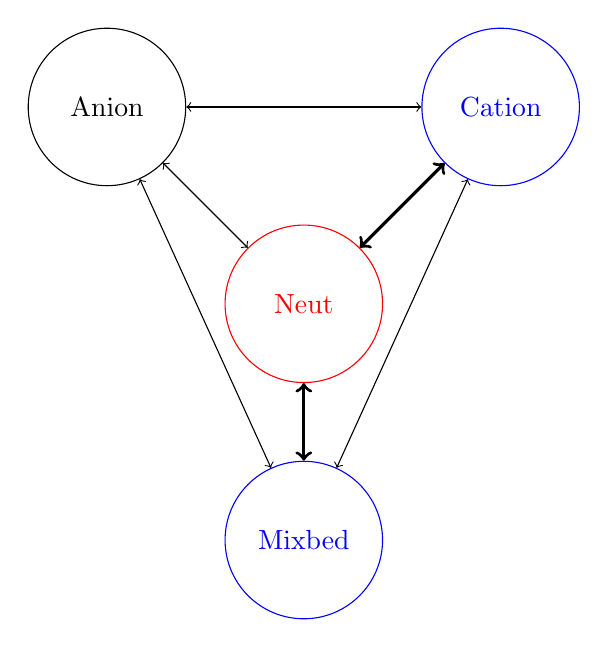
\begin{tikzpicture}
	\node[circle,draw, red, minimum size=2cm] (A) at  (0,0) {Neut};
	\node[circle,draw, minimum size=2cm] (B) at (-2.5,2.5) {Anion};
	\node[circle,draw, blue, minimum size=2cm] (C) at (2.5,2.5) {Cation};
	\node[circle,draw, blue, minimum size=2cm] (D) at (0,-3) {Mixbed};
	
	\draw[<->] (A) -- (B);
	\draw[very thick, <->] (A) -- (C);
	\draw[very thick, <->] (A) -- (D);
	\draw[<->] (B) -- (C);
	\draw[<->] (B) -- (D);
	\draw[<->] (C) -- (D);
	\end{tikzpicture}
	\caption{Acid negotiation. Red indicates seller, blue buyer. The Neut sells the acid, while the Cation and Mixbed agent try to obtain as much acid as possible.}
	\label{fig:agent-plant-acid}
\end{figure}

\begin{figure}[h]
	\centering
	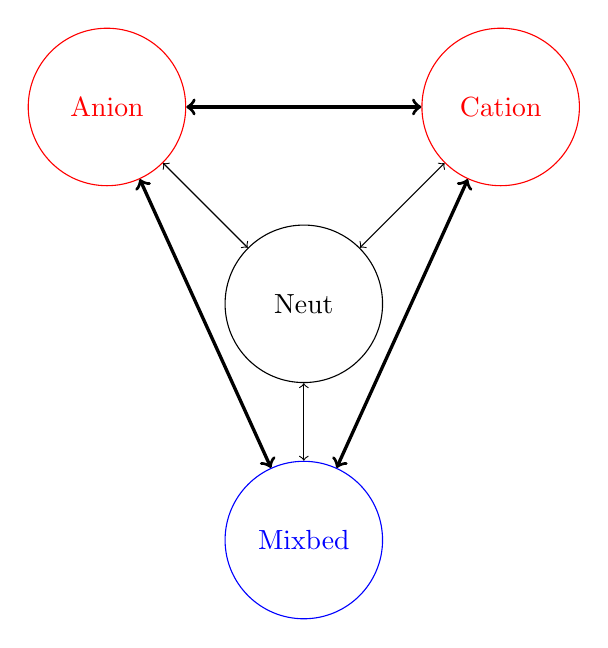
\begin{tikzpicture}
	\node[circle,draw,  minimum size=2cm] (A) at  (0,0) {Neut};
	\node[circle,draw, red, minimum size=2cm] (B) at (-2.5,2.5) {Anion};
	\node[circle,draw, red, minimum size=2cm] (C) at (2.5,2.5) {Cation};
	\node[circle,draw, blue, minimum size=2cm] (D) at (0,-3) {Mixbed};
	
	\draw[<->] (A) -- (B);
	\draw[<->] (A) -- (C);
	\draw[<->] (A) -- (D);
	\draw[very thick, <->] (B) -- (C);
	\draw[very thick, <->] (B) -- (D);
	\draw[very thick, <->] (C) -- (D);
	\end{tikzpicture}
	\caption{Water negotiation. Red indicates seller, blue buyer. The cation and anion sell water, while the Mixbed agent tries to obtain as much water as possible}
	\label{fig:agent-plant-water}
\end{figure}

So although there is a multi-issue negotiation, the only agent that has interest in all three issues is the Mixbed. This means that if an agent proposes 0.7 acid to the anion, the anion will not consider this part of the offer, as in since it can not project this to its' indifference curve. This means that the anions new proposal will also include 0.7 anion, and the adjusted values to the other issues.
\clearpage
\subsection{The solution space}
Below the solution space for the agents is shown, when $ru_i = 0.3$ for all agents.
\begin{figure}[h]
	\centering
	\begin{subfigure}[b]{0.4\textwidth}
		\centering
		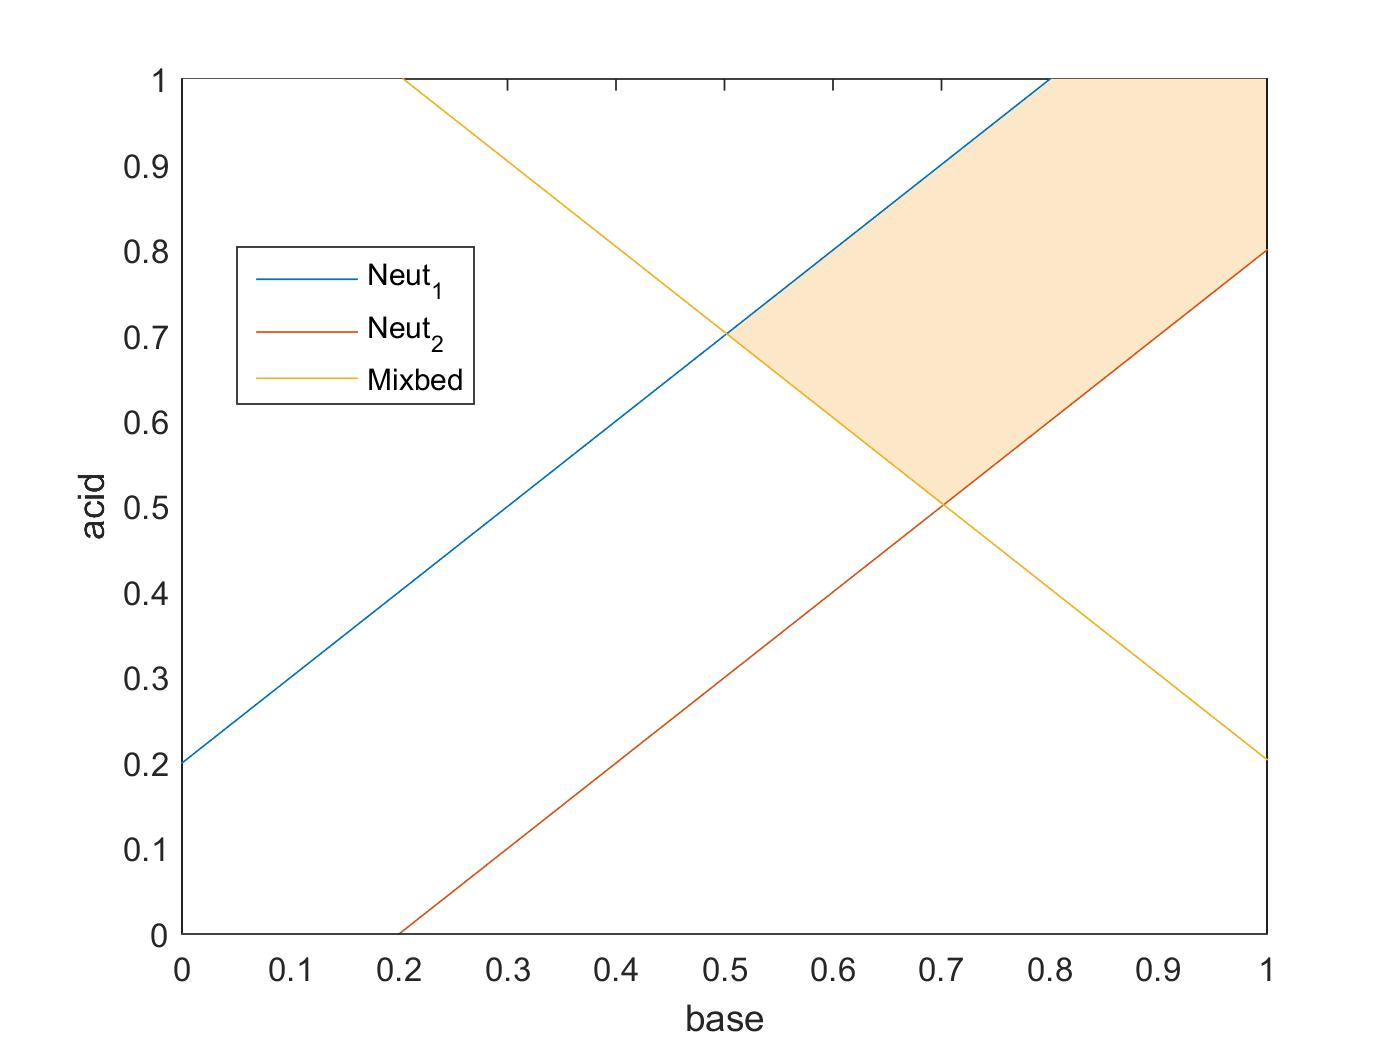
\includegraphics[width=\linewidth]{img/reservationcurve_base_acid}
		\caption{The solution space for the combination of acid and base}
		\label{fig:solutionbaseacid}
	\end{subfigure}
	~
	%~ %add desired spacing between images, e. g. ~, \quad, \qquad, \hfill etc. 
	%(or a blank line to force the subfigure onto a new line)
	\begin{subfigure}[b]{0.4\textwidth}
		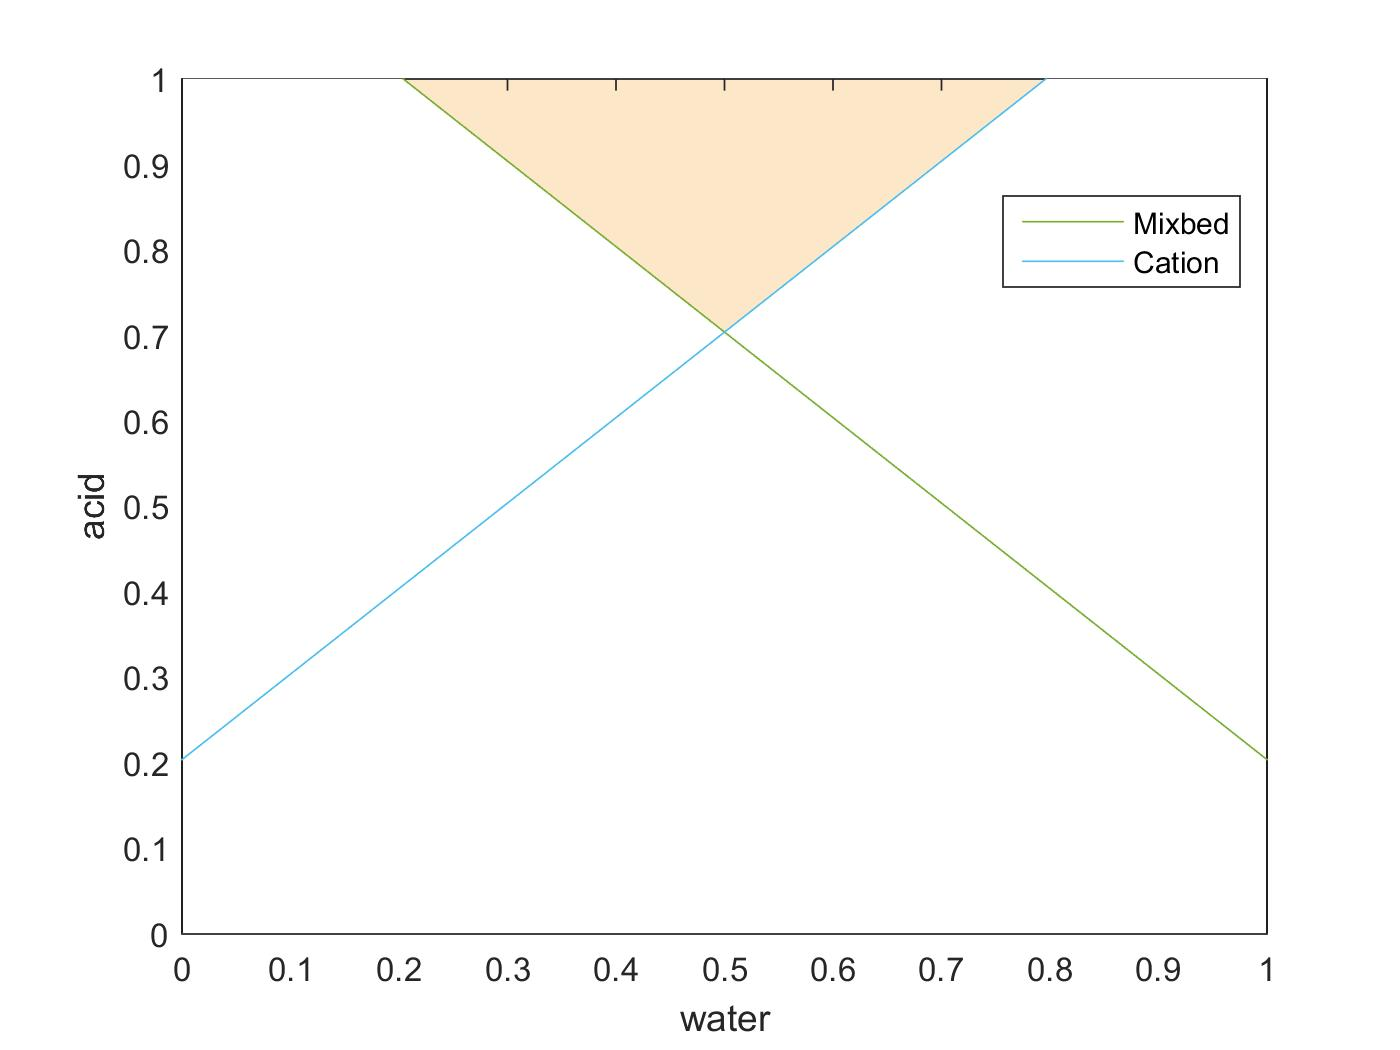
\includegraphics[width=\linewidth]{img/reservationcurve_water_acid}
		\caption{The solution space for the combination of acid and water}
		\label{fig:solutionwateracid}
	\end{subfigure}
	~
	%~ %add desired spacing between images, e. g. ~, \quad, \qquad, \hfill etc. 
	%(or a blank line to force the subfigure onto a new line)
	\begin{subfigure}[b]{0.4\textwidth}
		\centering
		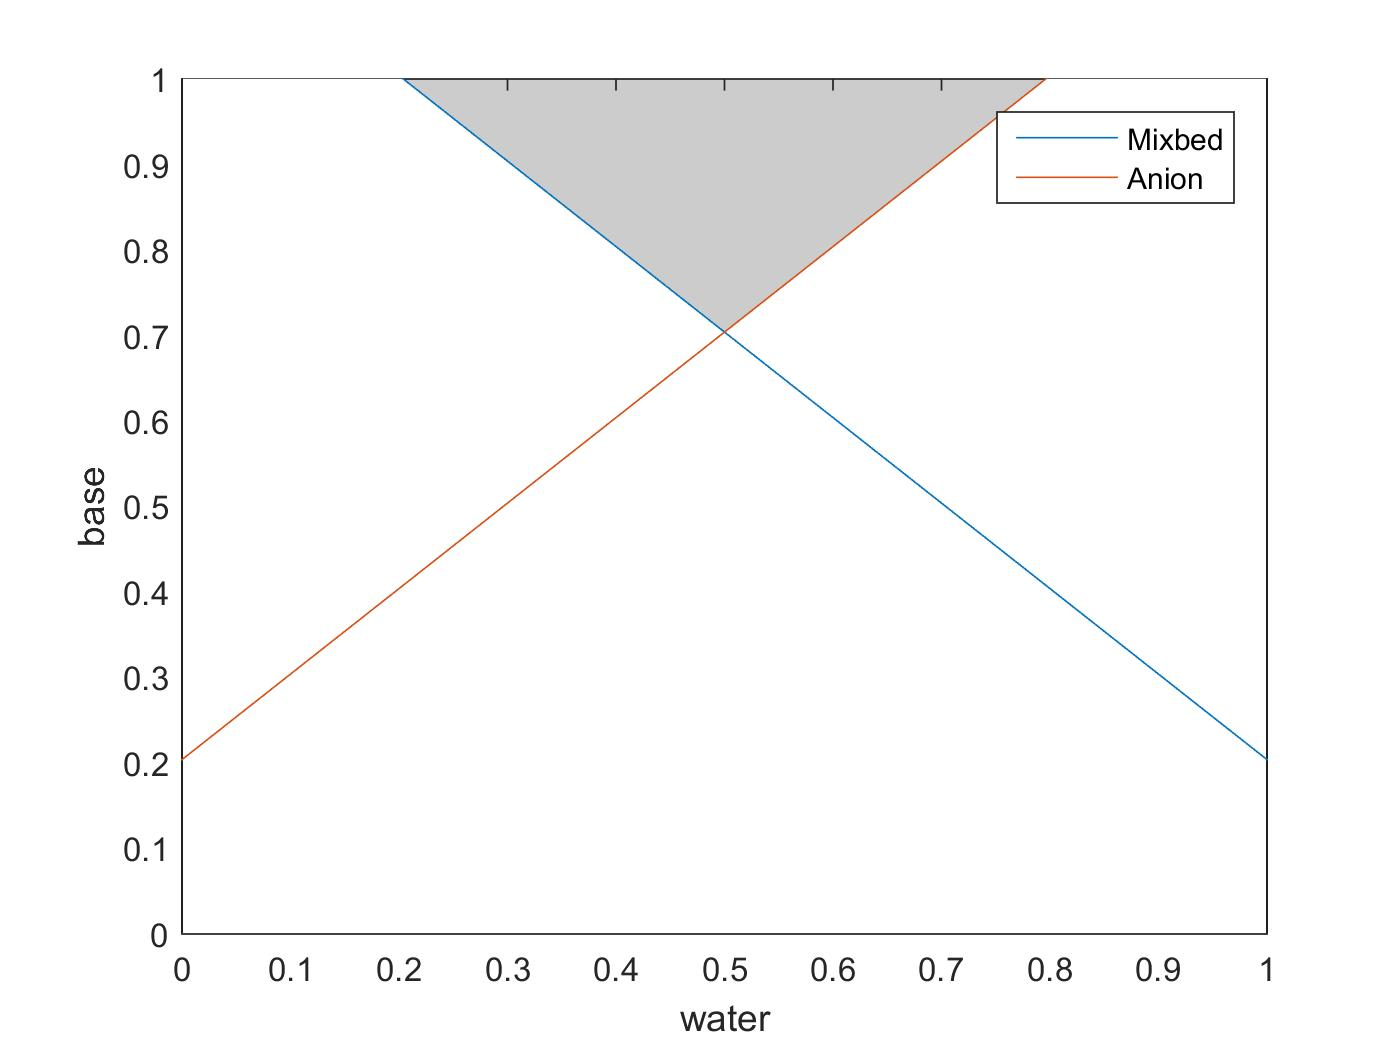
\includegraphics[width=\linewidth]{img/reservationcurve_water_base}
		\caption{The solution space for the combination of base and water, which are negotiated over by the anion and the Mixbed agent.}
		\label{fig:solutionwaterbase}
	\end{subfigure}
	\caption{The solution spaces for the different resources}\label{fig:solutionspace} 
\end{figure}

\clearpage
\section{Algorithm}
The algorithm, as programmed in Java is implemented using different objects. This was originally described in \Cref{ch:literature} as the optimal way to implement agents. The model consist of 4 different agents, which in turn can either be an anion, cation, Mixbed or neut with their own characteristics.

The algorithm starts with each agent proposing their preferred offer, which is the offer with their highest utility. After each agent proposes, the first agent starts with the generation of the offer. \Cref{al:algorithm1} shows the reactive concession strategy, but a non-reactive strategy is easily applied when changing \Cref{al:start} to $\text{if } true$.

Afterwards, depending on the concession protocol, their desired utility decreases, meaning that the proposal creeps towards the solution space as can be seen in \Cref{fig:searchforsolution}. 
\begin{figure}[h]
	\centering
	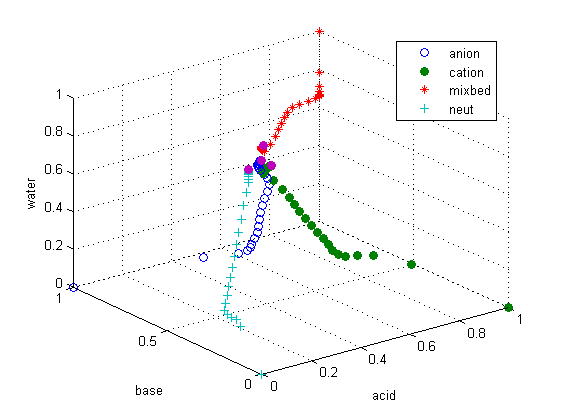
\includegraphics[width=0.7\linewidth]{img/searchforsolution}
	\caption{An example run of the agents searching for the solution. It is clearly seen that the agents start with their proposal in the corners, their optimal offers, and slowly make concessions towards eachother.}
	\label{fig:searchforsolution}
\end{figure}

%\todo[Todo Visualize algorithm results]{Visualize algorithm results.}
\begin{algorithm}[h]
	\KwData{Each agent's utility function $u_i(x)$, 
		reservation utility $ru_i$,
		and non-reactive concession strategy $s_i(t)= 1,2,...,T$}
	\KwResult{Negotiation Agreement}
	initialization: Each agent proposes a preferred offer $x^i_0$\;
	Each agent initializes these as previous best offer $x^k_{[j,-1]}$\;
	$t\leftarrow1$\;
	Set convergence tolerance: $\delta$\;
	\While{$t\leq T$ and IsConverge == False}
	{
		Determine the agent to propose: $i = \mod(t,4)$\;
		\ForEach{$j\in {1,2,3,4}$}
		{
			\eIf{j == i}
			{
				%Agent $i$ concedes by determining $s_i(t)$\:
				$\Delta u_{j0} = s^0_j(t)-s^0_j(t-1)$\;
				\ForEach{$k\in {1,2,3,4}$}
				{
					\eIf{$u_j(x^k_t) \geq ru_j$  \nllabel{al:start}}{
						$\Delta u_{jk} \leftarrow \Delta u_{j0}(t) $\;
					}{
						$\Delta_1 u_{jk}(t) \leftarrow u_j(x^k_t)-u_j(x^k_{[j,-1]})$\;
						$\Delta_2 u_{jk}(t) \leftarrow u_j(x^k_t)-u_j(x^k_0)-(1-u_j(x^j_{t-1}))$\;
						$\Delta u_{jk} \leftarrow \max \{\Delta_1u_{jk}(t), \Delta_2u_{j
							k}(t),0\}$\;
					}
					$\Delta u_j(t)\leftarrow \min \{\displaystyle \min_{k\in 1, 2, 3, 4}\Delta u_{jk}(t), \Delta u_{j0}(t)\}$ \nllabel{al:end}\;	
				}
				Agent $i$ concedes by determining $s_i(t)\leftarrow s_i(t-1)-\Delta u_j(t)$\;
				Agent $i$ calculates: $w_{t-1}\leftarrow \frac{1}{m}\sum_{j=1}^{m}x^j_{t-1}$\;
				Agent $i$ proposes $P_{A^i_t}[w_{t-1}]$\;
			}{
				$x^j_i \leftarrow x^j_{t-1}$\;
				\If{$u_j(x^i)_{t-1}\geq u_j(x^i_{[j,-1]})$}{
					$x^i_{[j,-1]}(t) \leftarrow x^i_{t-1}(t-1)$\;
				}
				$x^j_{[i,-1]}(t) \leftarrow x^j_{[i,-1]}(t-1)$\;
			}
		}
		\eIf{$\displaystyle \max_{ j \in {1,2,...,m}} \parallel x^j_t-w_{t-1} \parallel < \delta$ }
		{
			IsConverge $\leftarrow $ True\;
		}{
			$t \leftarrow t+1$\;
		}
	}
\caption{Basic algorithm structure modified from \citep{zheng2015automated}. Applied to the four agents which are used in this usecase.}
\label{al:algorithm1}
\end{algorithm}
\clearpage
\section{Result interpretation}
\label{sec:design:mean}
The outcome of the negotiation has to be translated to a value. We know the maximum production. Thus, 0.5 water means for example that 0.5 of the maximum water will be produced by the anion, cation and Mixbed. When an outcome of 0.7 for the acid is negotiated, this means that 0.7 of the possible acid has to be divided over the cation and Mixbed. We then devide this amount equally over the cation and Mixbed. However, if the Mixbed's water $l$ is set to 10, it also requires 10 times as little base than the anion filter i.e..

Thus, the allocation of the base to the anion and Mixbed is dependent on de water $l$. This is a fixed separation. Let's say the group agree to 0.6 usage of base. If $l$ is set to $1$, we allocate as much base to the Mixbed as the anion (0.3 each). However, if $l$ is set to 10, this means that the Mixbed will receive 1/11th of the base while the anion receives 10/11th. 

\section{Proof of convergence}
If there is an intersect of the agreement zone, the agents will find this.
This is already proven in the Zeuthen strategy \citep{rosenschein1994rules}, which shows that no agreement is always worse than a bad agreement. In infinite time this will happen. 

Furthermore, we have shown that the projection gives us the point closest to the agreement-set of an agent. Since it was proven by \citet{zheng2015automated} that if $x$ is projected on to the agreement-set  ($P_A[x]$), this also can be said of the projection on the linear line with the method used. 

%\todo[Euclidische meetkunde axiomas gebruiken?]{Euclidische meetkunde axiomas gebruiken?}
%\clearpage
%\section{Solution space}
%Below the solution space for the agents is shown, when $ru_i = 0.3$ for all agents. Each agent has 2 or three subjects 
%\begin{figure}[h]
%	\centering
%	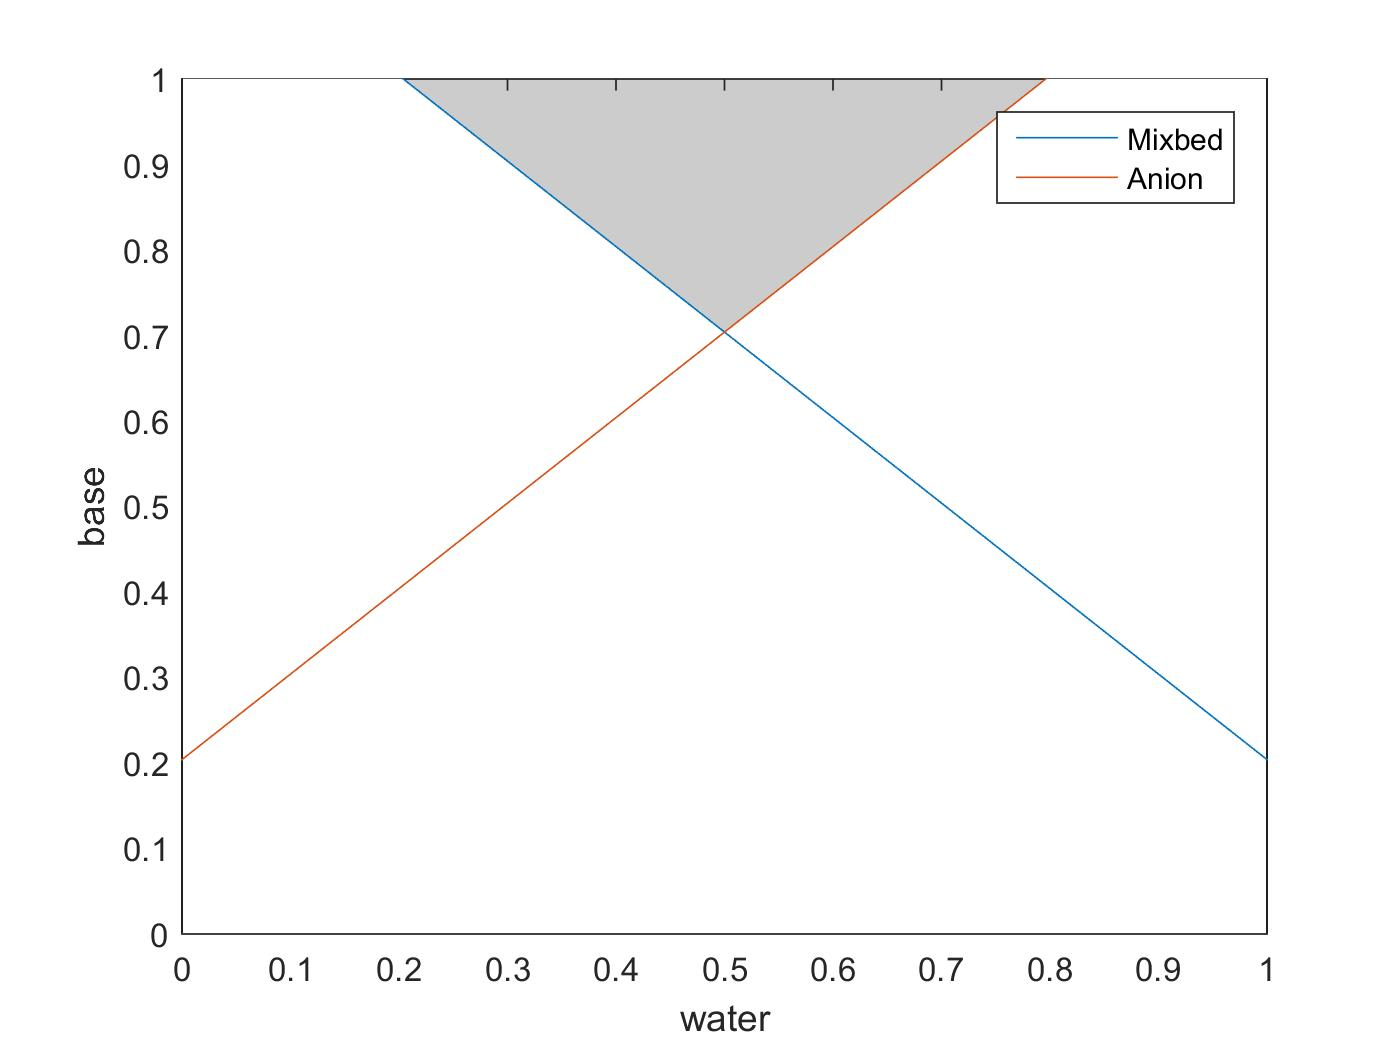
\includegraphics[width=0.7\linewidth]{img/reservationcurve_water_base}
%	\caption{The solution space for the combination of base and water, which are negotiated over by the anion and the Mixbed agent.}
%	\label{fig:reservationcurvewaterbase}
%\end{figure}
%
%\begin{figure}[h]
%	\centering
%	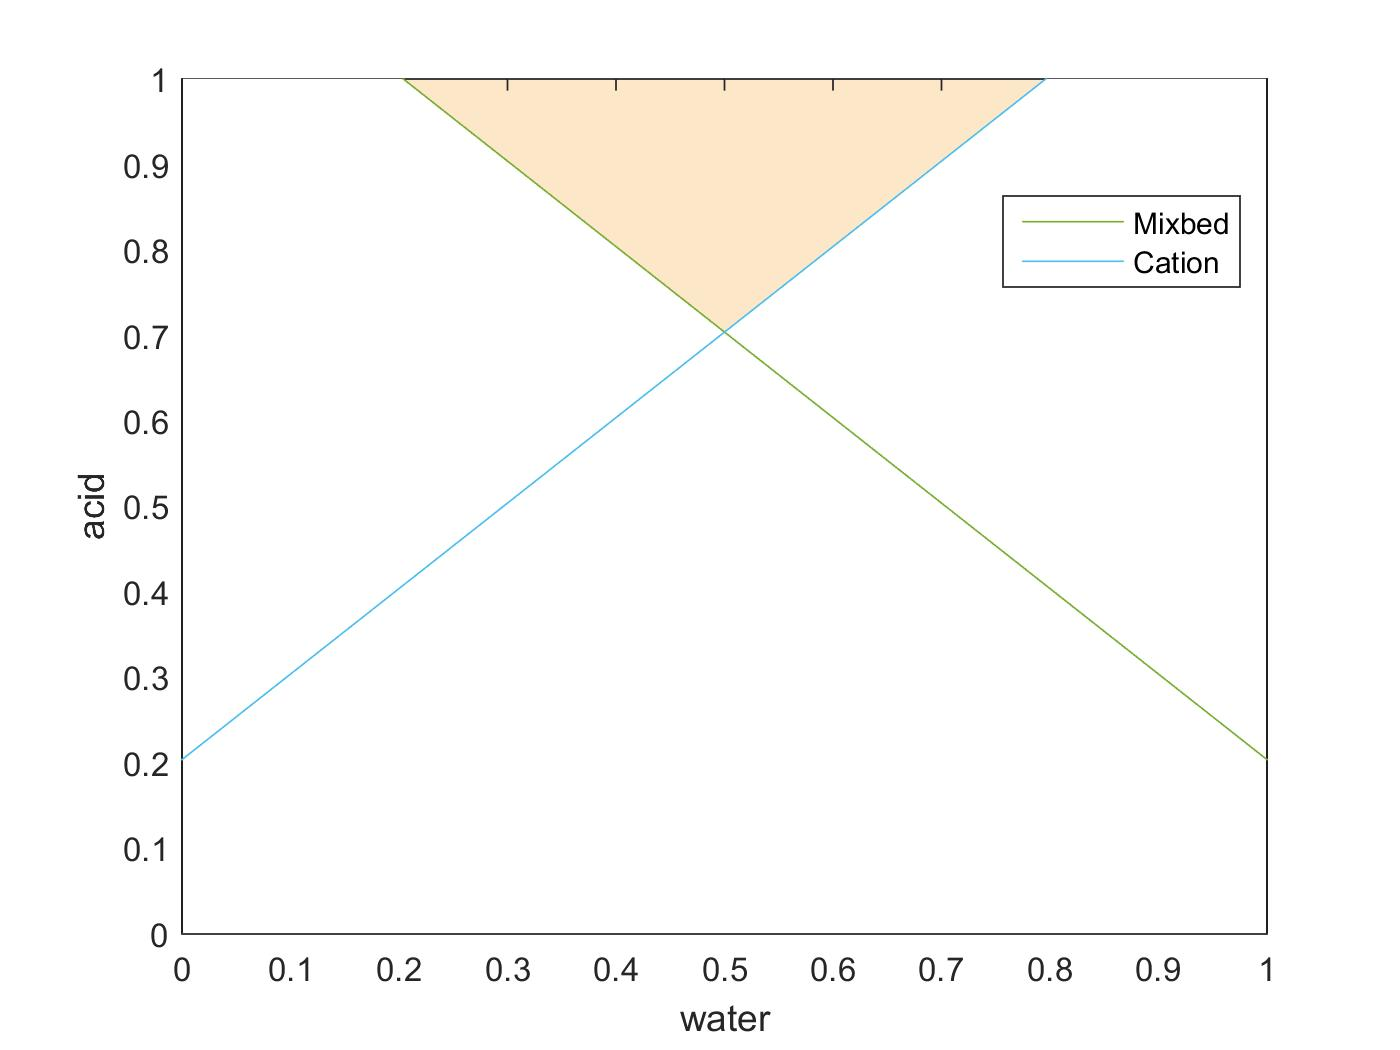
\includegraphics[width=0.7\linewidth]{img/reservationcurve_water_acid}
%	\caption{The solution space for the combination of acid and water}
%	\label{fig:reservationcurvewateracid}
%\end{figure}
%\begin{figure}[h]
%	\centering
%	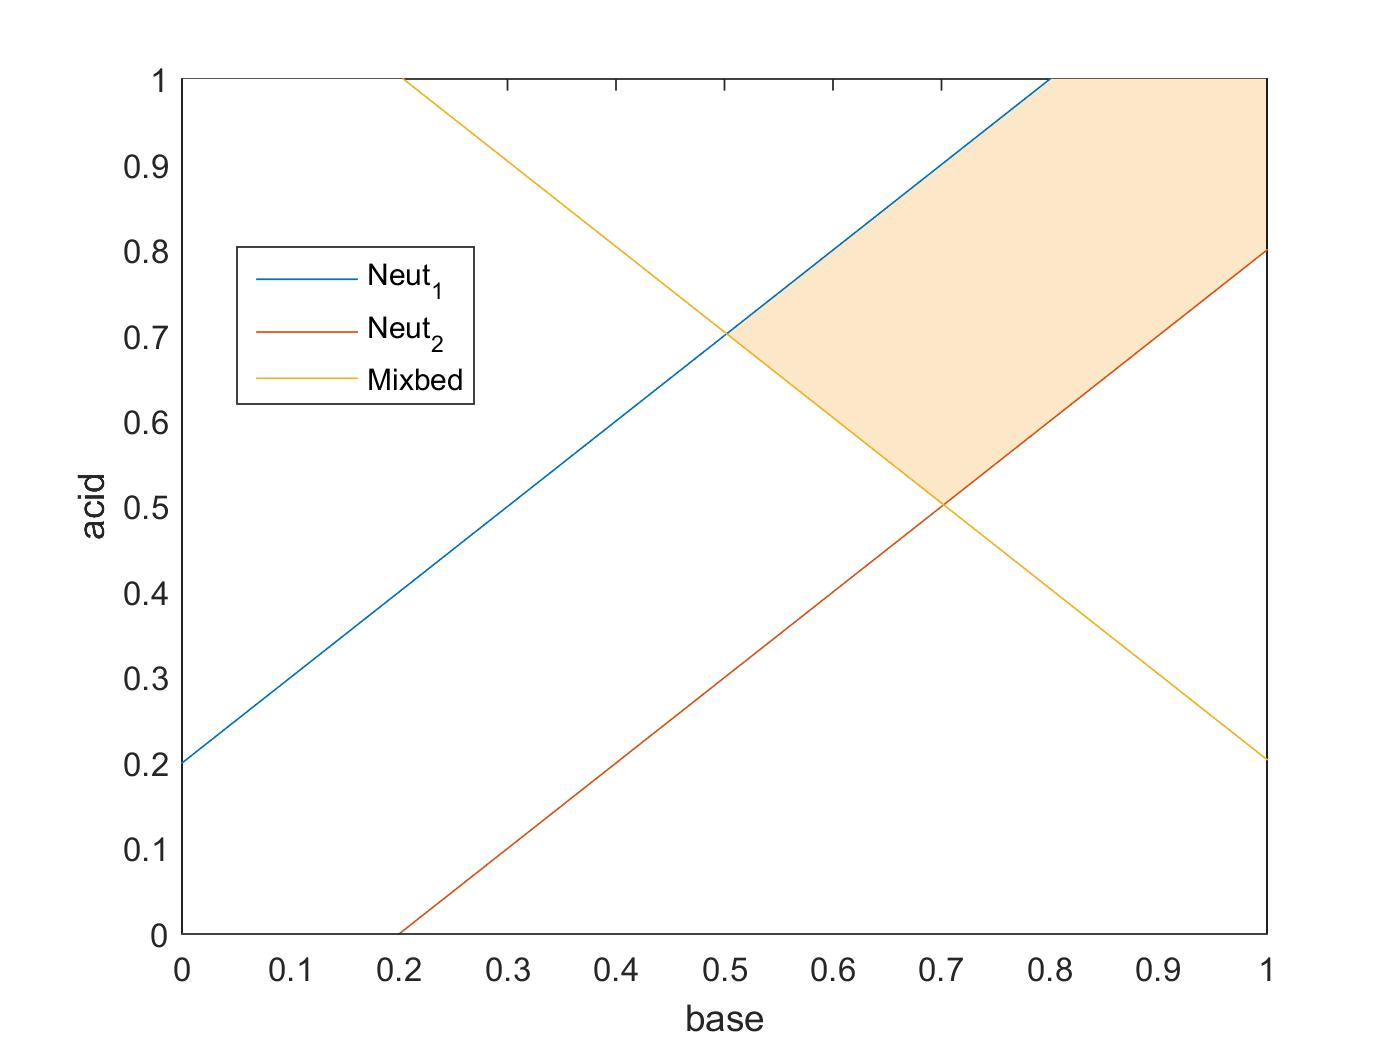
\includegraphics[width=0.7\linewidth]{img/reservationcurve_base_acid}
%	\caption{The solution space for the combination of acid and base}
%	\label{fig:reservationcurvebaseacid}
%\end{figure}
%



%\begin{figure}
%	\centering
%	\begin{tikzpicture}
%[domain=0.15:4]
%%\draw[very thin,color=gray] (0.01,0.01) grid (3.9,3.9);
%\draw[->] (0.02,0) -- (4.2,0) node[below] {$Water$};
%\draw[->] (0,0.02) -- (0,4.2) node[left] {$Base$}; %node[pos=0.25, left]   {$200 m^3 / hr$} 
%\draw[scale=0.5,domain=0.1:7.872,smooth,variable=\x,red] plot({\x},{(1/ (\x-8))+8 } );
%
%\end{tikzpicture}
%\label{fig:rcurveofanion}
%\caption{An illustrative sketch reservation curve of the offer space for the anion}
%\end{figure}



%The reservation function is shown in \Cref{fig:cationreservationfunction}.
%\begin{figure}
%	\centering
%	\begin{tikzpicture}[domain=0.15:4]
%	%\draw[very thin,color=gray] (0.01,0.01) grid (3.9,3.9);
%	\draw[->] (0.02,0) -- (4.2,0) node[below] {$Water$};
%	\draw[->] (0,0.02) -- (0,4.2) node[left] {$Acid$};% node[pos=0.25, left] {$200 m^3 / hr$};
%	\draw[color=black] plot (\x,{0.07*exp(\x)}) node[left] {$R_C$};
%	\end{tikzpicture}
%	\label{fig:cationreservationfunction}
%	\caption{The reservation function for the Cation filter: the more water is filtered and given, the more acid it requires.}
%\end{figure}




%\begin{figure}[h]
%	\centering
%	\begin{tikzpicture}
%	
%	\node[circle,draw,  minimum size=1cm] (C1) at  (0,0) {C$_1$};
%	\node[circle,draw,  minimum size=1cm] (C2) at  (0,-1.5) {C$_2$};
%	\node[circle,draw,  minimum size=1cm] (C3) at  (0,-3) {C$_3$};
%	\node[circle,draw,  minimum size=1cm] (C4) at  (0,-4.5) {C$_4$};
%	\node[circle,draw,  minimum size=1cm] (C5) at  (0,-6) {C$_5$};
%	\node[circle,draw,  minimum size=1cm] (C6) at  (0,-7.5) {C$_6$};
%	%\draw  (0,-2.5) ellipse (1 and 3.4);
%	
%	\node[ellipse,  draw, minimum height =9cm, minimum width = 2.5cm ] (C) at (0,-3.75) {Cation};
%	
%	\end{tikzpicture}
%	\caption{Cation head and sub-agents}
%	\label{fig:cation-head-sub}
%\end{figure}
%\subsubsection{Facts}
%The following facts and rules are part of the Anion.
%
%\begin{enumerate}
%	\item
%	Knowledge of cation head about the sub-agents:
%	\begin{itemize}
%		\item {$\{C_1, ..., C_6\}$ can process $a$ amount of water}
%		\item {$\{C_1, ..., C_6\}$ needs to be cleaned after $b$ water}
%		\item {$\{C_1, ..., C_6\}$ has filtered $c$ amount of water}
%		\item {$\{C_1, ..., C_6\}$ needs $d$ acid to clean}
%		\item {$\{C_1, ..., C_6\}$ needs $e$ time to clean}
%	\end{itemize}
%	\item
%	Currently $x$ amount of water being filtered 
%	\item
%	Currently $Z \subseteq \{C_1, ..., C_6\}$ filter being used for water filtering
%	\item
%	Currently $Y \subseteq \{C_1, ..., C_6\}$ filter being used for cleaning
%	\item
%	Currently $w$ amount of acid being used for cleaning
%\end{enumerate}
%
%\clearpage


%\begin{figure}[h]
%	\centering
%	\begin{tikzpicture}
%	
%	\node[circle,draw,  minimum size=1cm] (M1) at  (0,0) {M$_1$};
%	\node[circle,draw,  minimum size=1cm] (M2) at  (0,-1.5) {M$_2$};
%	\node[circle,draw,  minimum size=1cm] (M3) at  (0,-3) {M$_3$};
%	%\draw  (0,-2.5) ellipse (1 and 3.4);
%	
%	\node[ellipse,  draw, align=left, minimum height =5cm, minimum width = 2cm ] (A) at (0,-1.5) { \rotatebox{90}{\parbox{1cm}{Mixbed \\\\ \\ \\}}};
%	
%	\end{tikzpicture}
%	\caption{Mixbed head and sub-agents}
%	\label{fig:Mixbed-head-sub}
%\end{figure}


%\begin{figure}
%	\centering
%	\begin{tikzpicture}[domain=1.3:4]
%	%\draw[very thin,color=gray] (0.01,0.01) grid (3.9,3.9);
%	\draw[->] (0.02,0) -- (4.2,0) node[below] {$Water$};
%	\draw[->] (0,0.02) -- (0,4.2) node[left] {$Acid$};% node[pos=0.25, left] {$200 m^3 / hr$};
%	\draw[color=black] plot (\x,{(1/(\x-1))+1}) node[above] {$M_C$};
%	\end{tikzpicture}
%	\label{fig:mixreservationfunction1}
%	\caption{The reservation function for the Mixbed filter: a bear minimum of water is required at all times, and thus a bare minimum of cleaning acid.}
%\end{figure}

%
%
%\begin{figure}
%	\centering
%	\begin{tikzpicture}[domain=1.3:4]
%	%\draw[very thin,color=gray] (0.01,0.01) grid (3.9,3.9);
%	\draw[->] (0.02,0) -- (4.2,0) node[below] {$Water$};
%	\draw[->] (0,0.02) -- (0,4.2) node[left] {$Base$};% node[pos=0.25, left] {$200 m^3 / hr$};
%	\draw[color=black] plot (\x,{(1/(\x-1))+1}) node[above] {$M_C$};
%		\end{tikzpicture}
%		\label{fig:mixreservationfunction2}
%		\caption{The reservation function for the Mixbed filter: a bear minimum of water is required at all times, and thus a bare minimum of cleaning base.}
%	\end{figure}
%\subsubsection{Facts}
%The following facts and rules are part of the Mixbed.
%
%\begin{enumerate}
%	\item
%	Knowledge of anion head about the sub-agents:
%	\begin{itemize}
%		\item {$\{M_1, M_2, M_3\}$ can process $a$ amount of water}
%		\item {$\{M_1, M_2, M_3\}$ needs to be cleaned after $b$ water}
%		\item {$\{M_1, M_2, M_3\}$ has filtered $c$ amount of water}
%		\item {$\{M_1, M_2, M_3\}$ needs $d$ base to clean}
%		\item {$\{M_1, M_2, M_3\}$ needs $e$ time to clean}
%		\item {$\{M_1, M_2, M_3\}$ needs $f$ acid to clean}
%	\end{itemize}
%	\item
%	Currently $x$ amount of water being filtered 
%	\item
%	Currently $Z \subseteq \{M_1, M_2, M_3\}$ filter being used for water filtering
%	\item
%	Currently $Y \subseteq \{M_1, M_2, M_3\}$ filter being used for cleaning
%	\item
%	Currently $w$ amount of base being used for cleaning
%	\item
%	Currently $v$ amount of acid being used for cleaning
%\end{enumerate}

%\begin{figure}
%	\centering
%      \begin{tikzpicture}
%      
%      [domain = 0.1:3.9]
%      
%      \draw[->] (0.02,0) -- (4.2,0) node[right] {$Base$}; 
%      \draw[->] (0,0.02) -- (0,4.2) node[left] {$Acid$};
%      \draw[scale=0.5,domain=0:6,smooth,variable=\x,blue] plot ({\x},{\x+2}) node[left] {$R_{N1}$};
%      
%      \draw[scale=0.5,domain=2:8,smooth,variable=\x,blue] plot ({\x},{\x-2}) node[right] {$R_{N2}$} ;
%      
%      \end{tikzpicture}
%		\caption{The neut reservation curve. A near equal division is required.}
%		\label{fig:neutreservationcurve}
%\end{figure}
%\subsubsection{Facts}
%The following facts and rules are part of the Neut.
%
%\begin{enumerate}
%	\item
%	Current $a$ amount of acid being used.
%	\item
%	Current $b$ amount of base being used.
%	
%\end{enumerate}


%\begin{figure}
%	\centering
%\begin{tikzpicture}
%[domain=0.15:4]
%%\draw[very thin,color=gray] (0.01,0.01) grid (3.9,3.9);
%\draw[->] (0.02,0) -- (4.2,0) node[below] {$Water$};
%\draw[->] (0,0.02) -- (0,4.2) node[left] {$Acid$}; %node[pos=0.25, left]   {$200 m^3 / hr$} 
%\draw[scale=0.5,domain=0.1:7.872,smooth,variable=\x,blue] plot({\x},{(1/ (\x-8))+8 } );
%
%\end{tikzpicture}
%\label{fig:rcurveofcation}
%\caption{An illustrative sketch reservation curve of the offer space for the cation}
%\end{figure}

\chapter{Simulation Comparison and Evaluations}
\label{ch:eval}
In the previous chapter we have described our model, with the reactive concession strategy. Here the reactive concession strategy is compared to a non-reactive concession strategy. Furthermore, different values for the reservation utility are checked, and different values for the Mixbed agent water requirements are compared. 

\section{Parameters}
The parameters that are checked are compared to the baseline non-reactive strategy. Firstly the Nash solution is described to compare to the optimal solution. The parameters will be described in more detail.

\subsection{Nash Bargaining Solution}
The Nash bargaining solution is found using the product of agent's utility, maximizing the joint utility: $\prod_{i=i}^{m}u_i(x).$ We can calculate this since to us the utilities of the agent is known. This information is unknown to the agents since they only know their own utility curve. The joint utility gives the global maximum, and optimal Nash Solution. The utility functions of the agents are convex, which means that the solution is Pareto optimal and maximizes the product of the utilities \citep{nash1950bargaining, roth1977individual, lensberg1988stability}. 

\begin{alignat*}{2}
\text{maximize }   	& \prod_{i=1}^m u_i(x)  \\
\text{subject to \ } 	& u_i(x) \geq ru_i, & i = 1,...,m\\
& 0\leq x_j\leq 1, & j = 1,...,n\\
\end{alignat*}

Using the non-linear COUENNE program \citep{belotti2013mixed} implemented in GAMS \citep{GamsSoftware2013}, the solutions are calculated. The limit for the reservation curve is also found. This is dependent on the utility functions, but our default utility give a $\forall i,  ru_i = 0.3182$. This means that there is no solution space, if $\forall i, ru_i > 0.3182$. However, if only a single agent were to have a $ru_i > 0.3182$, there still would be a solution. This obviously depends on the reservation curve values of the other agents.

\subsection{Non-Reactive Concession Strategy}
As explained in \Cref{sec:concessionstrat} the concession strategy determines whether a solution will be found. If no concession is made during the negotiation, and the agent stay on their initial utility, no agreement can be made. In this result the non-reactive strategy is used as a base line to compare to other methods. As described, there are many methods, and a weak concession is used in here, since the utility functions of the other agents are unknown. The non-reactive concession strategy used is $s_i(t) = \max \{s_0(t) - t * 0.01, ru_i\}$. This monotonic decreasing concession is a linear function until the reservation value. Described by \cite{wu2009efficient}, it is an \textit{amount of utility}, where Agent $ i \in N$ concedes a fixed amount utility $au$. They found that it was well performing, and has the advantage of ending after a known number of rounds. Since the utility functions are private, utilitarian concessions are not possible \citep{endriss2006monotonic}. 

This means that the minimum utility value is reached after 100 rounds, if only the non-reactive concession strategy is used. Then each agent makes $\frac{100}{4 \text{agents}} = 25 \text{ proposals}$. Since we combine it with the reactive concession strategy, it is possible for the agents to negotiate for more rounds.

\subsection{Reactive Concession Strategy}
The reactive concession strategy (see \Cref{sec:reactiveconcessionstr} for an explanation) is compared to the non-reactive concession strategy. Similar to \citet{zheng2015automated}, however here different reservation utilities are checked, while comparing the reactive to non-reactive strategy.

\subsection{Reservation Curve}
The curve, as shown in \Cref{sec:design:negmod}, is not really a curve, but a linear limit. The values can differ from 	
$ru_i = \{0.05, 0.10, 0.15, 0.20, 0.25, 0.3, 0.35, 0.4, 0.45, 0.5, \\0.55, 0.6, 0.65\}$. We have seen that in the initial case, there is no agreement zone if the $ru_i$ is larger than $0.3182$. But, since we try different kind of parameters, it could be the case that if one of the reservation curves were to be different, the rest could as well. 

\subsection{Distance}
For the algorithm \Cref{al:algorithm1} to finish, there are two option. Either the distance from the offer and weight is smaller than a threshold, or the maximum number of rounds is reached. This distance, $ \displaystyle\max_{ j \in {1,2,...,m}} \parallel x^j_t-w_{t-1} \parallel$ gives the maximum distance from the agents to the weight. It tells something about the final solution and is thus used in the results to determine how the efficiency of the solutions. 

If the distance is larger than the threshold, it means that the agents have not found an agreement and the maximum number of rounds has been reached. The final solution will be the average of all proposals. Two options are possible. Either one or more agent(s) has not conceded and thus not moved to the agreement-zone. Another option is that the reservation utilities is too high, meaning that there is no agreement-zone, and thus no agreement possible. 

Since we know where the agreement zone lies, we can see when the agent(s) do not concede, and thus refrain from agreement if the distance is larger than the threshold.


\subsubsection{Threshold \& Maximum Number of Rounds}
As shown in the algorithm, there is a threshold required to decide on the value and whether an agreement is reached. For this simulation this is set to $\delta = 0.05$.	The maximum number of rounds is set to $200$.

Since the non-reactive concession give a maximum of 100 rounds until zero is reached, 200 seems as an overkill. However, since we are dealing with the combination of different concession strategies, it is useful to check whether a solution is found afterwards. This since there might change something in the proposals due to the reactive concession method. If the non-reactive method were to be changed, it would be important to change the number of rounds as well. 

So if the number of rounds is equal to 199, no agreement has been made.

\section{Reactive Compared to the Non-Reactive Concession Strategy}
When comparing the reactive to the non-reactive strategy, as shown in \Cref{fig:reactivevsnon-reactive}, it is obvious that the Nash limit indeed lies at $ru_i = 0.3182$. However, unexpectedly, the non-reactive strategy consequently finds the solution closer to the optimal Nash Bargaining Solution then the reactive strategy. For completeness, the Nash solution lies at acid $= 0.571$, base $= 0.571$, water $= 0.714$.

\begin{figure}[h]
	\centering
	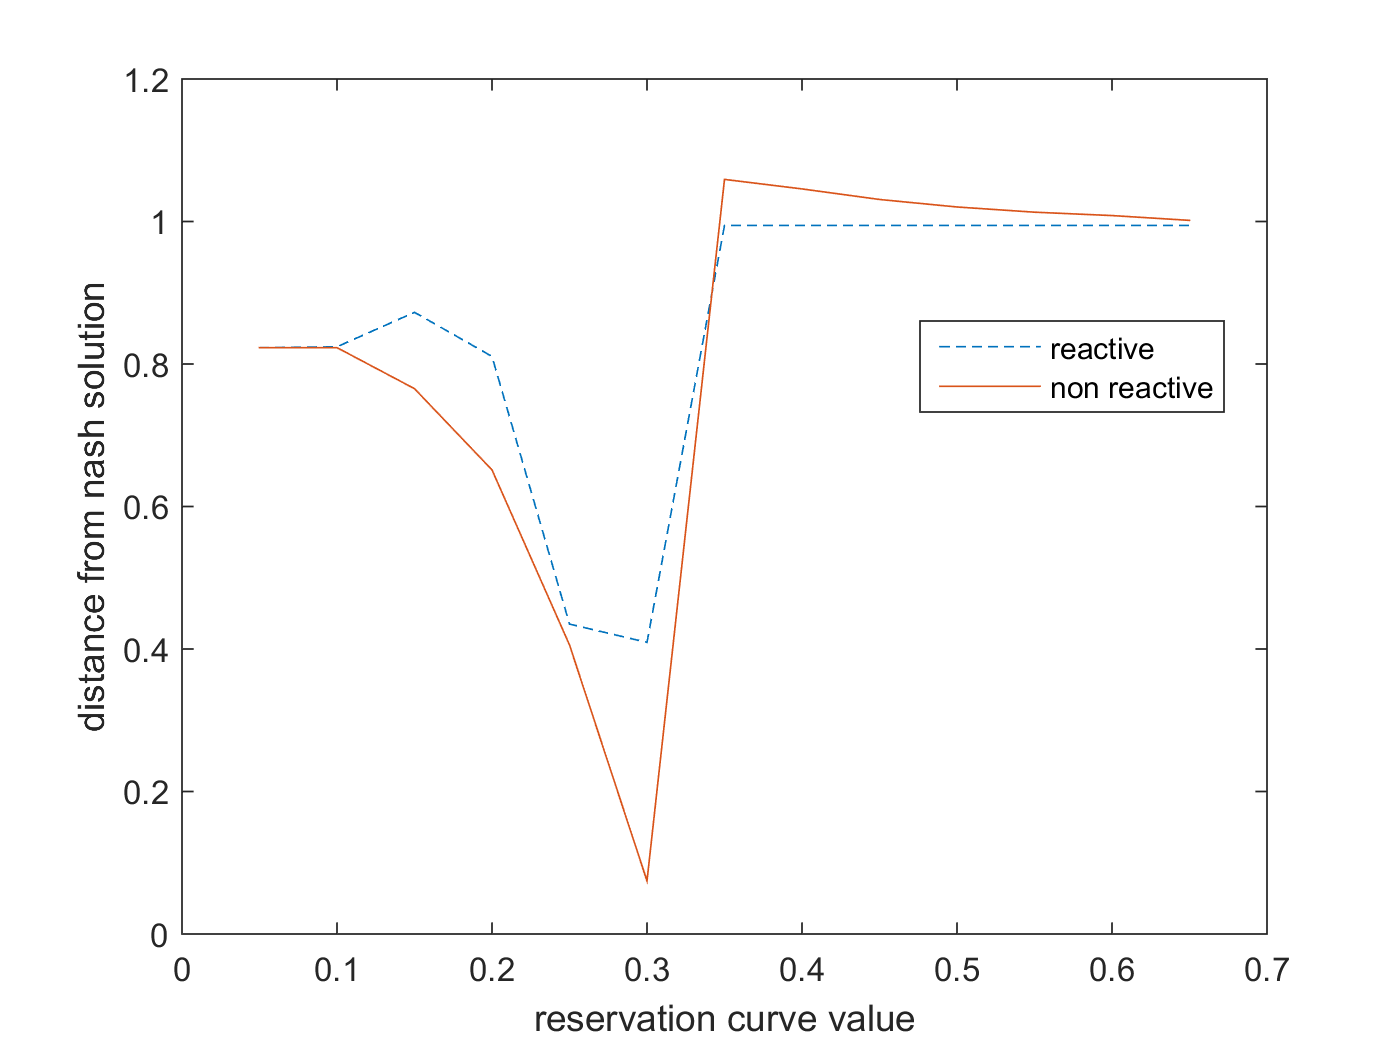
\includegraphics[width=0.9\linewidth]{img/reactivevsnonreactive}
	\caption{Distance from the Nash bargaining solution for the reactive and non-reactive concession strategies. }
	\label{fig:reactivevsnon-reactive}
\end{figure}

\npdecimalsign{.}
\nprounddigits{4}
\begin{table}[h]
\begin{tabular}{|l|n{1}{4}|c|n{1}{4}|c|}\toprule
	&	\multicolumn{2}{|c|}{Reactive concession}&\multicolumn{2}{|c|}{Non-reactive concession}\\
	\cmidrule{2-5}
{{reservation utility}}	& {{distance}} & {{\# of rounds}}  & {{distance}} & {{\# of rounds}} \\ 
	\hline 
0.05&	0&				26&		0.0295631273025621&		23\\
0.10&	0&				26&		0.0295631273025621&	 	23\\
0.15&	0&				38&		0.0295631273025621&	 	23\\
0.20&	0&				50&		0.0295631273025621&	 	23\\
0.25&	1.06932375691321&199&	0.0295631273025621&		23\\
0.30&	1.17512099855347&199&	0.0485167717872400&		66\\
0.35&	1.17163511966245&199&	0.127686769276389 &		199\\
0.40&	1.16753472222222&199&	0.279876154743691 &		199\\
0.45&	1.16753472222222&199&	0.425372845848635 &		199\\
0.50&	1.16753472222222&199&	0.555524071073009 &		199\\
0.55&	1.16753472222222&199&	0.673260175537175 &		199\\
0.60&	1.16753472222222&199&	0.780744817700835 &		199\\
0.65&	1.16753472222222&199&	0.874525088634732 &		199\\
\hline
\end{tabular} 
\caption{The distance in the final proposal and number of rounds of a simulation.}
\label{tab:reactivevsnon-reactive}
\end{table}
\npnoround

It can be seen that the non-reactive concession strategy halts after less rounds than the reactive concession strategy, which means that it is faster. The reactive concession strategy has a larger distance than the threshold, which means that there is no agreement, since the distance is larger than 0.05, and the number of rounds is 199. However, when looking at the distance from the reactive concession, it is zero, which means that the average is exactly the same as the proposals. Interestingly when looking at the distance from the optimal solution, \Cref{fig:reactivevsnon-reactive}, it is very large. This unexpected result will be discussed later. 
\clearpage
\section{Reactive Mixbed with other Agents Non-Reactive }
Although the reactive concession strategy performed worse when compared to the non-reactive concession strategy, a comparison to is made when only the Mixbed agent uses the reactive strategy. The Mixbed agent is the most important agent since it ``produces'' the final demi water product, the most important resource of the production line.

In the comparison of the Nash Bargaining Solution, in \Cref{fig:reactivevsnon-reactivevsnon-reactivemxbrea} it is seen that reactive Mixbed  method initially performs better than the reactive strategy. 


\begin{figure}[h]
	\centering
	\includegraphics[width=0.9\linewidth]{img/reactivevsnonreactivevsMixbedrea}
	\caption{Comparison of the reactive and non-reactive vs only reactive mixb}
	\label{fig:reactivevsnon-reactivevsnon-reactivemxbrea}
\end{figure}

When we look at the table, the only reactive Mixbed performs better than than when all the agent use the reactive concession protocol. 
\npdecimalsign{.}
\nprounddigits{4}
\begin{table}[h]
	\centering
\begin{tabular}{|c|n{1}{4}|c|}
	\hline 
	reservation utility	& {distance} & \# of rounds \\ 
	\hline 
	0.05&	0.0295631273025621	&23\\
	0.10&	0.0295631273025621	&23\\
	0.15&	0	&27\\
	0.20&	0.0482097633193126	&38\\
	0.25&	0.0442587760929785	&46\\
	0.30&	0.0348568605891333	&54\\
	0.35&	0.563115215004291	&199\\
	0.40&	0.685601610104541	&199\\
	0.45&	0.789500931992561	&199\\
	0.50&	0.926270897277326	&199\\
	0.55&	1.02930993557596	&199\\
	0.60&	1.11322894186644	&199\\
	0.65&	1.13049432160727	&199\\
	\hline
\end{tabular} 
\caption{The distance in the final proposal and number of rounds of a simulation. This is where only the Mixbed makes reactive concessions, and the other agents make non-reactive concessions. }
\label{tab:reactivevsnon-reactivevsMixbedrea}
\end{table}
\npnoround

\clearpage
\section{Changing the $l$ value for the Mixbed}
In the design it was stated that the water ratio to the base and acid could change for the Mixbed. Here an example is given where the Mixbed water to base and acid ratio is 2:1:1 and 10:1:1. Here a new Nash solution has to be calculated, since the utility functions have changed. So in the graph comparison, the Mixbed water with the updated ratio, is checked against the reactive and non-reactive concession strategies.

\subsection{Mixbed Ratio 2:1:1}
When looking at the first ration of 2:1:1, we get very similar result as that of the comparison. The minimum $rui$ lies way lower however, and has an maximum of $\forall i, ru_i = 0.301$. The Nash solution lies at acid = 0.600, base = 0.600, water = 0.800.
It is interesting to note that the new original end proposal is a lot nearer to the Nash solution than the base line situation when the reservation utility is low as can be seen in \Cref{fig:reactivevsnon-reactiveMixbed2}. Again the non-reactive concession strategy comes closer to the Nash solution ultimately, however initially the reactive concession strategy is better. 
\begin{figure}[h]
	\centering
	\includegraphics[width=0.7\linewidth]{img/reactivevsnonreactiveMixbed2.png}
	\caption{Comparison of the reactive and non-reactive strategy for a 2:1:1 ratio for the Mixbed. This compared to the original ratio of 1:1:1}
	\label{fig:reactivevsnon-reactiveMixbed2}
\end{figure}


\npdecimalsign{.}
\nprounddigits{4}
\begin{table}

\begin{tabular}{|l|n{1}{4}|c|n{1}{4}|c|}
	\hline 
		&	\multicolumn{2}{|c|}{Reactive concession}&\multicolumn{2}{|c|}{Non-reactive concession}\\
	\cline{2-5}
	{{reservation utility}}	& {{distance}} & {{\# of rounds}}  & {{distance}} & {{\# of rounds}} \\ 
	\hline 
0.05 & 0                 & 26  & 0                  & 26  \\
0.10 & 0                 & 30  & 0                  & 26  \\
0.15 & 0                 & 43  & 0                  & 26  \\
0.20 & 0.950693168831420 & 199 & 0                  & 26  \\
0.25 & 1.11331450231946  & 199 & 0                  & 26  \\
0.30 & 1.24151874372075  & 199 & 0.0472373495100384 & 71  \\
0.35 & 1.24001645374814  & 199 & 0.282988815136597  & 199 \\
0.40 & 1.23596954345703  & 199 & 0.452220659395809  & 199 \\
0.45 & 1.23596954345703  & 199 & 0.677438159537665  & 199 \\
0.50 & 1.23596954345703  & 199 & 0.779689267474365  & 199 \\
0.55 & 1.23596954345703  & 199 & 0.862468304051885  & 199 \\
0.60 & 1.23596954345703  & 199 & 0.926781060892920  & 199 \\
0.65 & 1.23596954345703  & 199 & 0.985943062172507  & 199\\
\hline
\end{tabular}
\label{tab:Mixbed2}
\caption{Here Mixbed ratio is water 2:1:1. }
\end{table}
\npnoround


\subsection{Mixbed Ratio 10:1:1}
When using a ratio of 10:1:1 we have a maximal reservation curve of: $ru_i = 0.274$. The Nash solution lies at acid $= 0.647$, base $= 0.647$, and water $=0.941$. The large increase to the water demand makes this an interesting solution. It is very interesting to note that although the reservation minimum lies at $0.274$, the algorithm still finds a solution very close to the Nash optimum when the reservation utility is 0.3. 
%\section{All}

\begin{figure}[h]
	\centering
	\includegraphics[width=0.7\linewidth]{img/reactivevsnonreactive_Mixbed10}
	\caption{Comparison of the reactive and non-reactive strategy for a 10:1:1 ratio for the Mixbed}
	\label{fig:reactivevsnonreactiveMixbed10}
\end{figure}

\npdecimalsign{.}
\nprounddigits{4}
\begin{table}[h]
	\centering
\begin{tabular}{|l|n{1}{4}|c|n{1}{4}|c|}
	\hline 
	&	\multicolumn{2}{|c|}{Reactive concession}&\multicolumn{2}{|c|}{Non-reactive concession}\\
\cline{2-5}
{{reservation utility}}	& {{distance}} & {{\# of rounds}}  & {{distance}} & {{\# of rounds}} \\ 
\hline 
0.05 & 0                & 34  & 0                  & 26  \\
0.10  & 0                & 38  & 0                  & 30  \\
0.15  & 0                & 59  & 0                  & 30  \\
0.20  & 1.01017004837544 & 199 & 0.0375849182069237 & 47  \\
0.25  & 1.18451892325133 & 199 & 0.0403767460130609 & 59  \\
0.30  & 1.28304255654208 & 199 & 0.196731504342998  & 199 \\
0.35  & 1.30000 & 199 & 0.516805014278959  & 199 \\
0.40  & 1.30000 & 199 & 0.620662764097981  & 199 \\
0.45  & 1.30000 & 199 & 0.712271791830695  & 199 \\
0.50  & 1.30000 & 199 & 0.794218859564544  & 199 \\
0.55  & 1.30000 & 199 & 0.868348999412338  & 199 \\
0.60  & 1.30000 & 199 & 0.936024514848705  & 199 \\
0.65  & 1.30000 & 199 & 0.998279954150336  & 199\\
\hline
\end{tabular}
\label{tab:Mixbed10}
\caption{The distance in the final proposal and number of rounds of a simulation. Here the Mixbed ratio is 10:1:1. }
\end{table}
\npnoround
%\begin{figure}
%	\centering
%	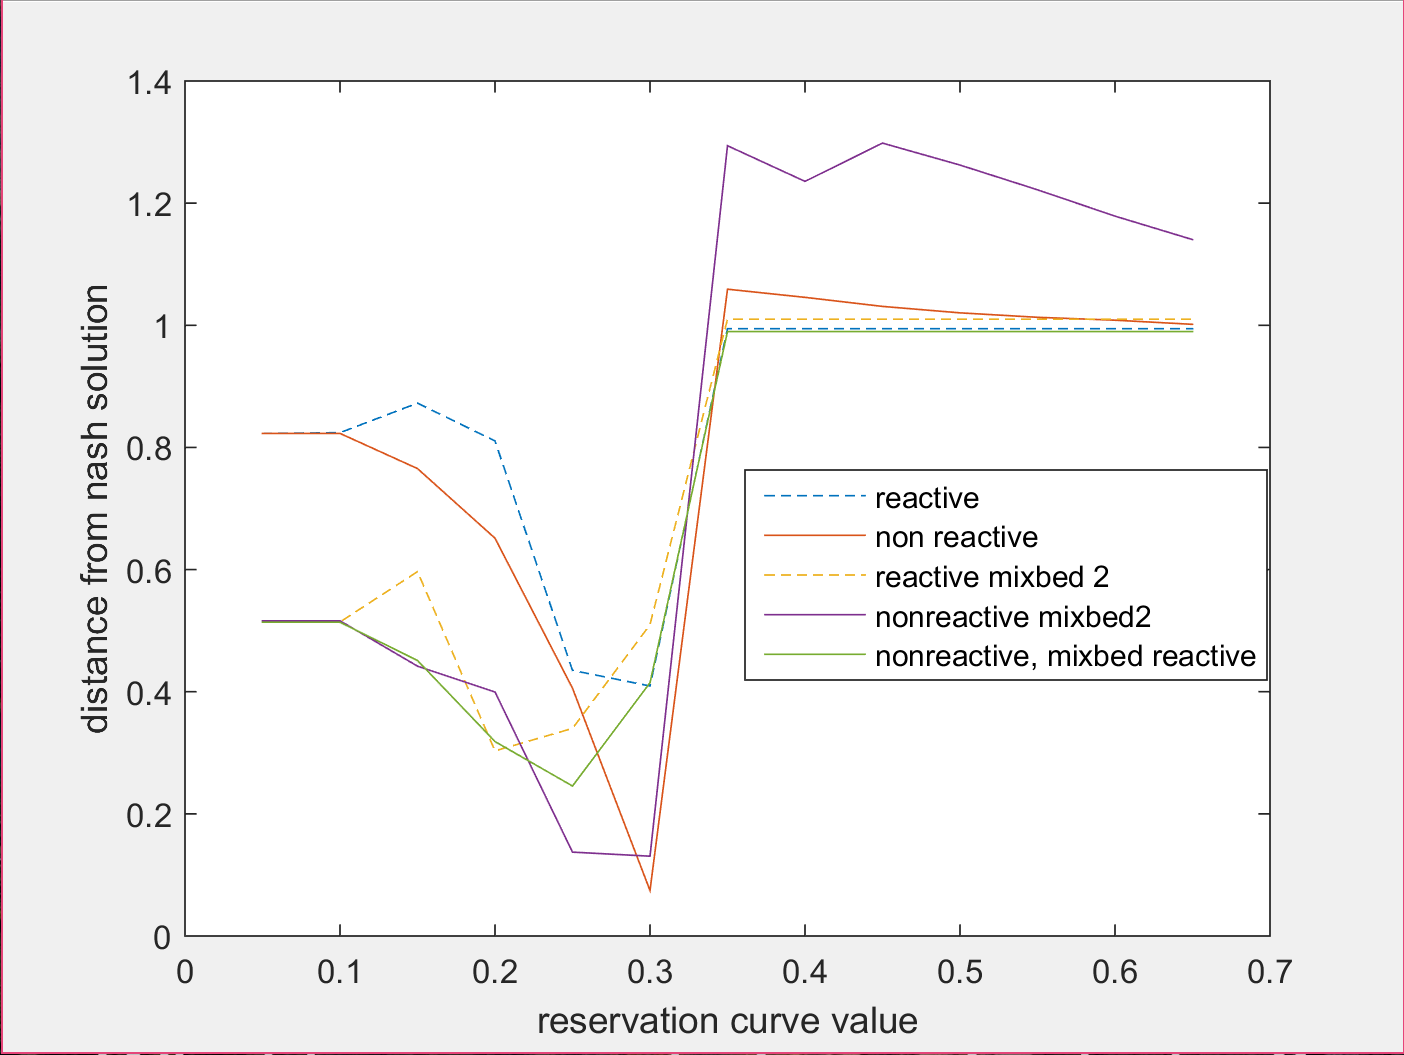
\includegraphics[width=0.7\linewidth]{img/all_dist_from_nash_solutions}
%	\caption{All plots fromthe nash solutions.}
%	\label{fig:alldistfromnashsolutions}
%\end{figure}

\clearpage
\section{Evaluation}
Since some unexpected results are seen, some possible explanations are given.
\subsection{Reactive compared to the non-reactive concession strategy}
It is interesting that the reactive concession strategy does not find a solution although there is an agreement-zone. 
A possible solution is that the answer cannot be found as is stated by \citet{zheng2015automated} as Lemma 2. ``If Agent $i$ deliberately stops conceding before reaching the agent's own reservation utility from time period t onward, and all other agents use the reactive concession strategy the negotiation will stall; i.e. other agents will reactively stop conceding and there will be no agreement if $\Delta_j < s_j(t)-u_j(x^*_{ru_i}) \text{ and } u_j(x^*_{s_i(t)})<ru_j$''.

As discussed, we see that the reactive concession strategy takes more rounds to find  This can be simply attributed to fact that the concession made each round is the $\displaystyle \min\{ \min_{j \in m}\Delta u_{ij} \delta u_i\}$, meaning that it is the minimum of the reactive and non-reactive concession. Thus, the concession will always smaller or equal to the non-reactive concession, and thus it will take longer to find a solution.

It is still possible in some rare cases that the negotiation may stall if it happens that none of the agents concede. The possibility may be higher for linear utility as it is a weak form of convexity. To reduce the possibility, it may work by revising algorithm 2 such that use $K_{ij}(t)$ to count the times that it happens that $max{ \Delta_1 u_{ij},\Delta_2 u_{ij}, 0 } == 0$ until time $t$, and assign $\Delta_{ij}(t) =  \Delta u_{i0}/(2^K_{ij}(t))$. This form of fraction would make the non-reactive concession protocol a form of the fraction protocol as described by \citet{wu2009efficient}.

\subsubsection{Situation at the 0.2 $ru$}
So as shown in the results there is an unexpected distance from the Nash solution in the situation of the 0.2 reservation curve for the reactive concession strategy. This can mostly be attributed to the stalling of the agents while trying to find a solution.

Looking at the proposals, \Cref{fig:reactive4plot}, it is clearly seen that in the reactive process the Neut and Mixbed do not react to the proposals of the Anion and Cation. After multiple proposals they finally start conceding, but not before the anion and cation have started to move towards the average of the Neut en Mixbed. 

\begin{figure}[h]
	\centering
	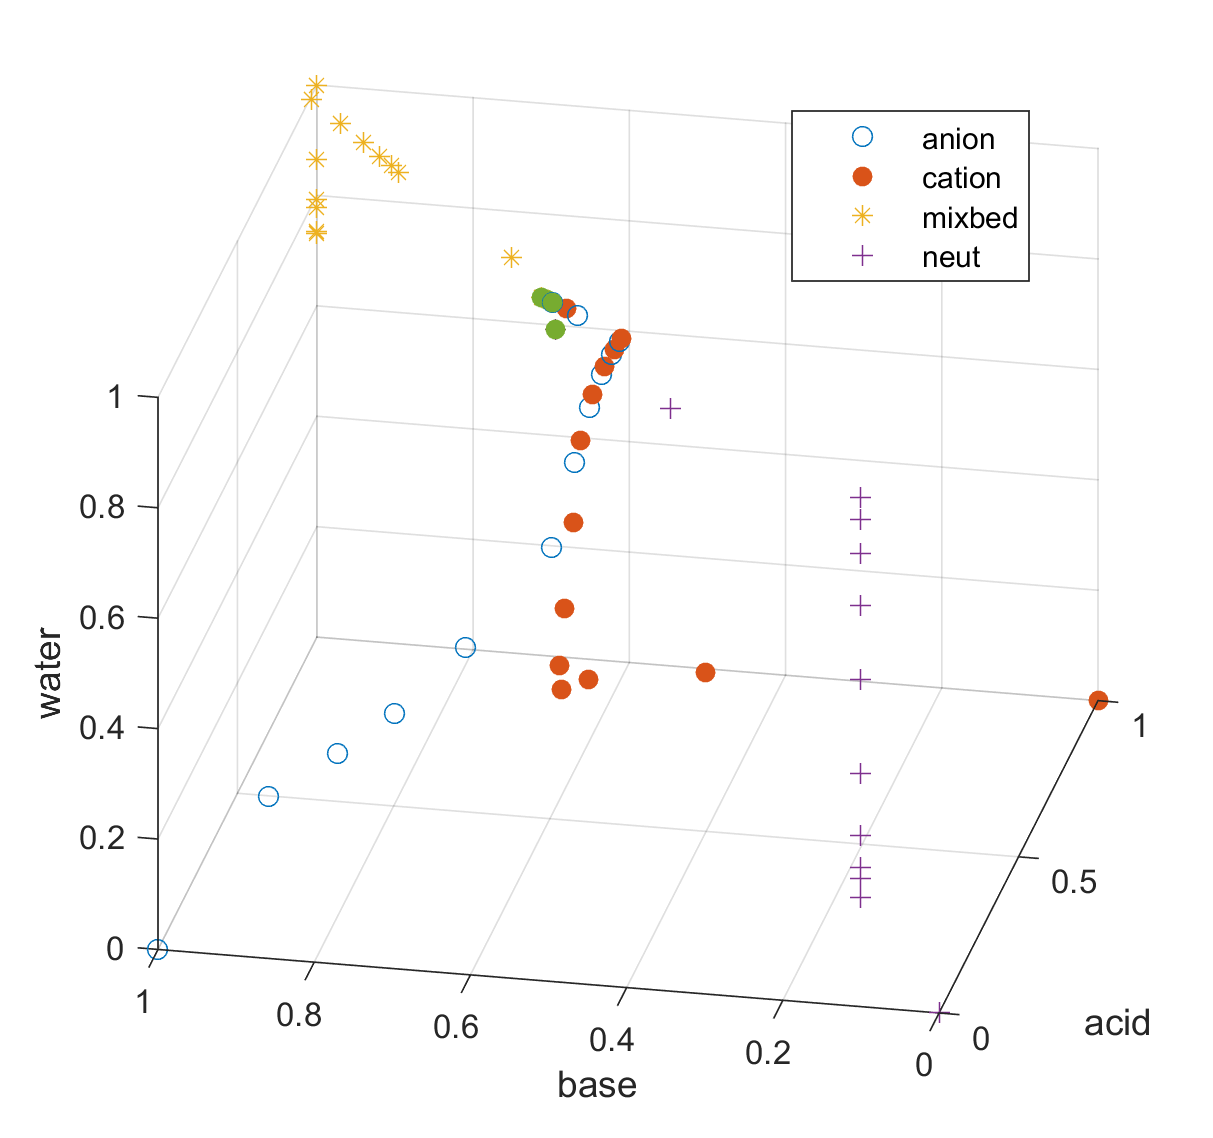
\includegraphics[width=0.7\linewidth]{img/reactive_4_plot}
	\caption{The proposals made by the 4 agents. We see that the Mixbed and neut ``stall'' in de finding of the solution. Only towards the end do they start conceding.}
	\label{fig:reactive4plot}
\end{figure}

The stalling of the Neut and Mixbed can also clearly be seen when looking at the desired utility of the agents. No concessions are made by the Neut and Mixbed until the end.

\begin{figure}[h]
	\centering
	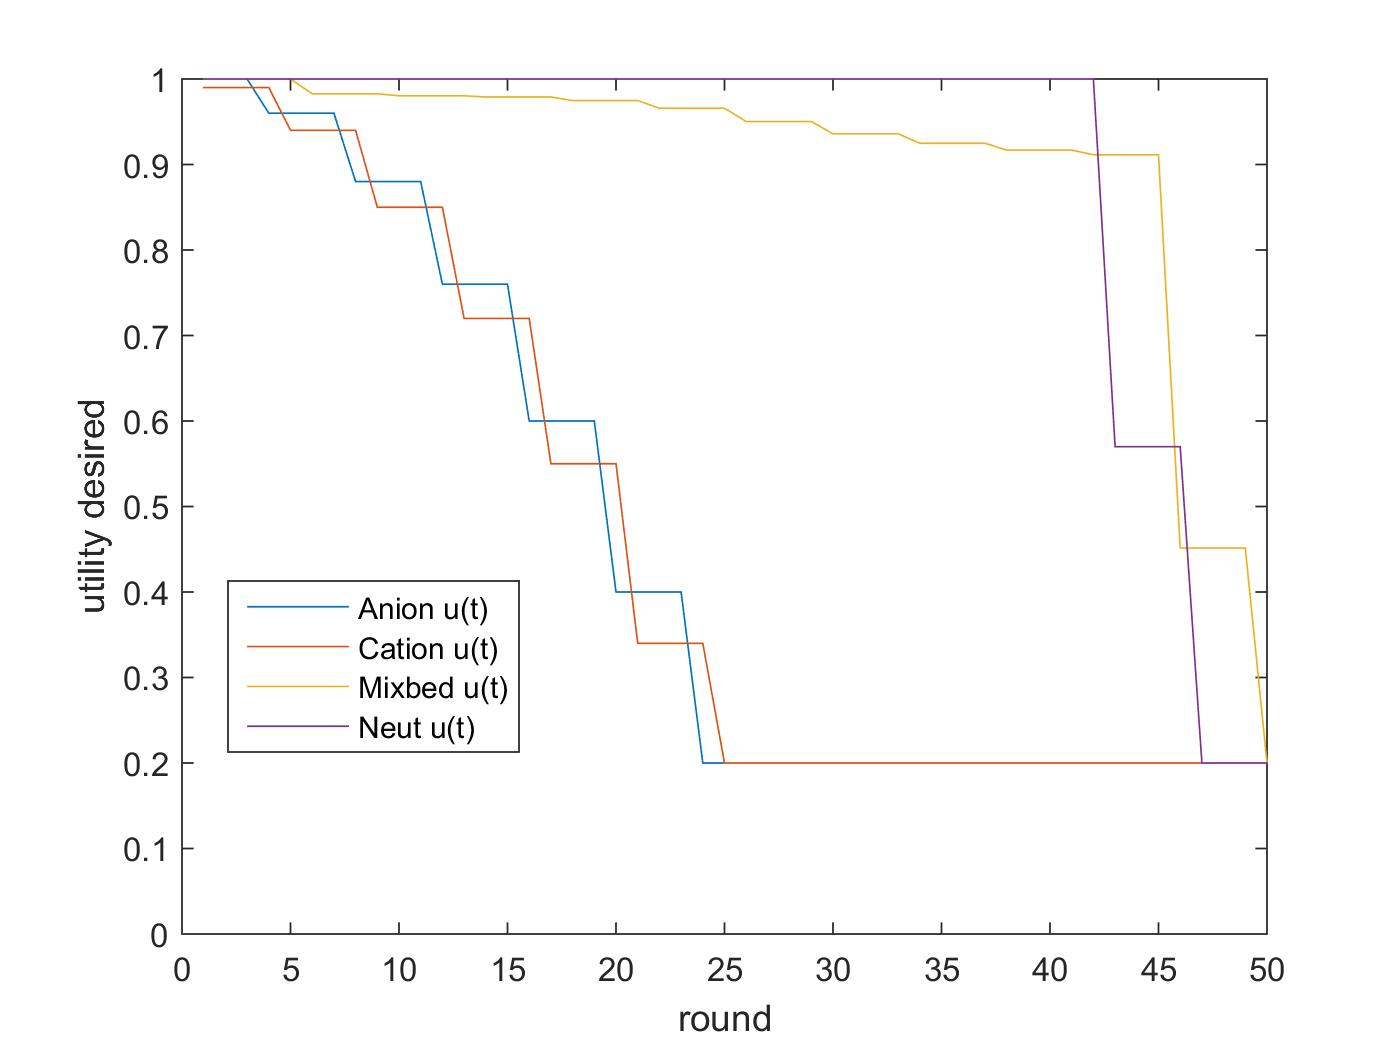
\includegraphics[width=0.7\linewidth]{img/desiredutility_reactive_4}
	\caption{The desired utility for the agents. The stall can be clearly seen for the Mixbed and neut agent. Only towards the end do they start conceding.}
	\label{fig:desiredutilityreactive4}
\end{figure}



\clearpage
\subsection{Reactive Mixbed compared to non-reactive other agents}
When we look at the solution which is found when only the Mixbed makes reactive concessions, we see that this is a lot more optimal than when all the agents use the reactive concession strategy. 

When this usecase is to be implemented in the real situation, using the reactive Mixbed is a realistic option. 

\subsection{Different values for $l$}
When looking at the different values of $l$, we see the exact same pattern as we saw in the original reactive vs non-reactive. So although the Nash solution moves, we still get an sub-optimal solution, where the non-reactive method outperforms the reactive method on distance to Nash, average and rounds necessary.

This means that the usage of ratios for the Mixbed are a very realistic solution to solve the problem of desire, when a sudden increase of output is necessary. This also solves the realistic problem of the Mixbed requiring a lot less cleaning than the anion and cation.



\chapter{Conclusion and Further Work}
To conclude we discuss our research, and give possible further research options.
\section{Conclusion}
In this thesis we have given an overview of agent solutions used in the manufacturing world. We found that a gap lies in the ``real'' negotiation, which excludes the use of auctions and or contract net protocol. By using the alternating offer protocol it is checked whether an optimal solution can be found. At the moment, it seems as if the reactive concession strategy, as described in \citet{zheng2015automated} still has some difficulties. This can be clearly seen in \Cref{fig:reactivevsnon-reactive}. 

So although it ensures that the agents only concede when the other agents concede, it under-performs However, when looking at the individual utility of an agent, it might be the best protocol to implement since it ensures that an agent only concedes if the other agents do as well.

The usage of private utility functions allows for competing companies to use automated negotiation. This is in line with the idea of Industrie 4.0, where companies specialize, but require products from other  producers. By implementing automated negotiation, without the requirement of releasing the utility functions, competing businesses can flourish together. This is conform to the principled negotiation ideology, which allows an optimal outcome.

\section{Discussion}
Although the alternating offer has been used, it is not usable at all yet at a real case. The largest difficulty lies in the realistic portrayal of the utility function. The requirement for a convex utility function makes it even more difficult. However, if only the non-reactive strategy was used, it should be possible to use a non-convex function.

In the literature we have discussed the concept of principled negotiation. There we discussed the importance of retaining a private utility function, but making it very important ot create this utility functions. This we have achieved, and thus we can say that the negotiation in this thesis is a form of principled negotiation.

In the problem statement we discussed the option of optimizing a production process using negotiation. We can conclude that this has not fully been achieved. We have looked at the implementation of multilateral multi-issue negotiation, without a mediator, and using a very simplified theoretical solution, this is achieved. 

A difficulty is that no concession is seen if an agent concedes in a matter that the other agents has no desire in. So if for example the cation concedes in the amount of water to produce (which means that it will produce more water), this concession will not be ``seen'' by the Neut, since it has no desire in this utility. %This makes it a possible undesirable method for the other agents, or .

A large flaw in the reactive concession strategy is that an agent can simply propose new offers on its utility curve without making a concession. The other agent can see this as a concession and make a concession. This results in uneven distributed concessions made. 

How can energy and manufacturing companies use the AI concept of intelligent multi-agent systems (MAS) for the optimization of production process.

The use case was not an optimal situation for the research. This due to the fact that the agents had no purpose to keep their utility private. This addition would have had more impact when looking at processes that require privacy.

Example is the interaction between pedestrians, cars, public transport at an interjection. Future asks for 

\section{Further research}
A lot of further research could be done on the alternating offer protocol to be used in manufacturing world. The agents could be improved to allow reasoning, using a holonic structure for example. Furthermore, other strategies can be used, while the utility functions can be changed as well. Extra negotiation could be applied using bilateral negotiations, and to finalize heuristic learning methods can be applied.

\subsection{Holonic agents}

This structure is that of a holon as can be seen in \Cref{fig:holonexample}. As shown in the literature it is based on PROSA by \citep{van1998reference}. Idealy this could be implemented in this usecase to make use of the different parts of the anion filter.
\begin{figure}[h]
	\centering
	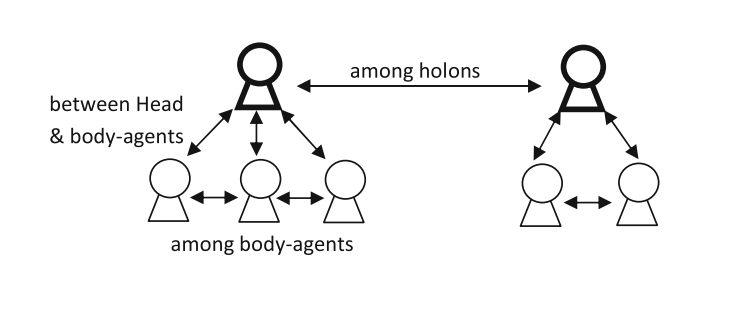
\includegraphics[width=0.7\linewidth]{img/holon_example}
	\caption{An example of the different negotiation between holons from \citet{beheshti2016negotiations}.}
	\label{fig:holonexample}
\end{figure}


\begin{figure}[h]
	
	\centering
	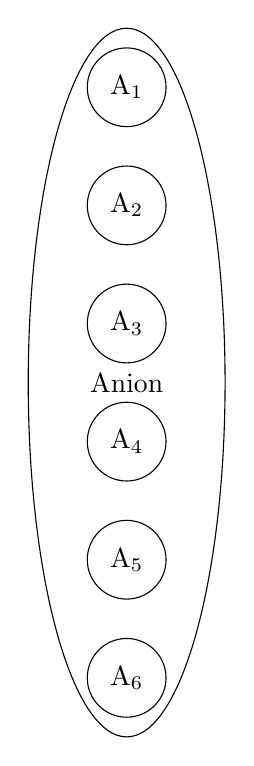
\begin{tikzpicture}
	
	\node[circle,draw,  minimum size=1cm] (A1) at  (0,0) {A$_1$};
	\node[circle,draw,  minimum size=1cm] (A2) at  (0,-1.5) {A$_2$};
	\node[circle,draw,  minimum size=1cm] (A3) at  (0,-3) {A$_3$};
	\node[circle,draw,  minimum size=1cm] (A4) at  (0,-4.5) {A$_4$};
	\node[circle,draw,  minimum size=1cm] (A5) at  (0,-6) {A$_5$};
	\node[circle,draw,  minimum size=1cm] (A6) at  (0,-7.5) {A$_6$};
	%\draw  (0,-2.5) ellipse (1 and 3.4);
	
	\node[ellipse,  draw, minimum height =9cm, minimum width = 2.5cm ] (A) at (0,-3.75) {Anion};
	
	\end{tikzpicture}
	\caption{Anion head and sub-agents}
	\label{fig:anion-head-sub}
	
\end{figure}

The following facts and rules would than be part of the Anion, meaning that a beginning towards an BDI in the agent can be made.

\begin{enumerate}
	\item
	Knowledge of anion head about the sub-agents:
	\begin{itemize}
		\item {$\{A_1, ..., A_6\}$ can process $a$ amount of water}
		\item {$\{A_1, ..., A_6\}$ needs to be cleaned after $b$ water}
		\item {$\{A_1, ..., A_6\}$ has filtered $c$ amount of water}
		\item {$\{A_1, ..., A_6\}$ needs $d$ base to clean}
		\item {$\{A_1, ..., A_6\}$ needs $e$ time to clean}
	\end{itemize}
	\item
	Currently $x$ amount of water being filtered 
	\item
	Currently $Z \subseteq \{A_1, ..., A_6\}$ filter being used for water filtering
	\item
	Currently $Y \subseteq \{A_1, ..., A_6\}$ filter being used for cleaning
	\item
	Currently $w$ amount of base being used for cleaning
\end{enumerate}

The use of these holons could allow an agent to reason about the environment, and act upon it accordingly.

\subsection{Utility function}
The requirement of a convex function forced the use of a specific, and highly theoretical function. This could be perfected using more expert input. Although an attempt was made, using a variable in the Mixbed ratio, this of course still is a highly theoretical and unrealistic representation.
\subsubsection{Reservation curve}
We have used a linear reservation curve for simplicity, since this eliminated the minimization (mixed integer programming) that would have been necessary if a truly curved function was used. An example is shown in \Cref{fig:anionreservationfunction}.
\begin{figure}[h]
	\centering
	\begin{tikzpicture}[domain=0.15:4]
	%\draw[very thin,color=gray] (0.01,0.01) grid (3.9,3.9);
	\draw[->] (0.02,0) -- (4.2,0) node[below] {$Water$};
	\draw[->] (0,0.02) -- (0,4.2) node[left] {$Base$};% node[pos=0.25, left] {$200 m^3 / hr$};
	\draw[color=black] plot (\x,{0.07*exp(\x)}) node[left] {$R_A$};
	\end{tikzpicture}
	\label{fig:anionreservationfunction}
	\caption{The reservation function for the Anion filter: the more water is filtered and given, the more base it requires.}
\end{figure}
\clearpage
\subsection{Continue negotiation after group agreement}
After the group has an agreement, the agents now allocate the resource as predefined (see \Cref{sec:design:mean}). This could be optimized to bilateral negotiation between the agents. Take the Mixbed and Anion for example: so if the group agrees to an allocation of 0.5 base, the Mixbed and anion can further negotiate how much of this 0.5 should be allocated to whom. This new bilateral negotiation is simpler, and due to the fact that it only contains a single issues, allows for quick determination.

\subsection{Extra concession strategies}
The many concession strategies, as shown in \Cref{sec:concessionstrat} allow for many strategies to be used. Further research could include using fraction, which was suggested as a good solution by \citet{wu2009efficient}. 
\subsection{Heuristic learning methods}
As shown in \Cref{sec:lit:learn}, heuristic learning methods can also be used to learn the desired utility function. This has not been done since the requirement of a convex utility functions forced the usage of predefined functions.
\newpage
\bibliographystyle{plainnat}
\bibliography{./bib/MAS_thesis}

\end{document}          
